\documentclass[dvipsnames]{article}
\usepackage{marvosym}
\usepackage{marvosym}

%...TikZ & PGF
\usepackage{pgfplots}
\pgfplotsset{compat=1.11}
\tikzset{>=latex}
\usetikzlibrary{calc,math}
\usepackage{tikzsymbols}
\usepgfplotslibrary{fillbetween}
\usetikzlibrary{decorations.markings} 
\usetikzlibrary{arrows.meta} %...APP2 for arrows as objects and images
\usetikzlibrary{backgrounds} %...For shading portions of graphs
\usetikzlibrary{patterns} %...Unit 5 Problems
\usetikzlibrary{shapes.geometric} %...For drawing cylinders in Unit 2
\tikzset{
    mark position/.style args={#1(#2)}{
        postaction={
            decorate,
            decoration={
                markings,
                mark=at position #1 with \coordinate (#2);
            }
        }
    }
} %...See https://tex.stackexchange.com/questions/43960/define-node-at-relative-coordinates-of-draw-plot

\tikzset{
    declare function = {trajectoryequation10(\x,\vi,\thetai)= tan(\thetai)*\x - 10*\x^2/(2*(\vi*cos(\thetai))^2);},
    declare function = {trajectoryequation(\x,\vi,\thetai)= tan(\thetai)*\x - 9.8*\x^2/(2*(\vi*cos(\thetai))^2);},
    declare function = {patheq(\x,\yi,\vi,\thetai)= \yi + tan(\thetai)*\x - 9.8*\x^2/(2*(\vi*cos(\thetai))^2);},
    declare function = {patheqten(\x,\yi,\vi,\thetai)= \yi + tan(\thetai)*\x - 10*\x^2/(2*(\vi*cos(\thetai))^2);} %like patheq but with gravity = 10
}

%...siunitx
\usepackage{siunitx}
\DeclareSIUnit{\nothing}{\relax}
\def\mymu{\SI{}{\micro\nothing} }
\DeclareSIUnit\mmHg{mmHg}
\DeclareSIUnit{\mile}{mi}
%...NOTE: "The product symbol between the number and unit is set using the quantity-product option."

%...Other
\usepackage{amsthm}
\usepackage{amsmath}
\usepackage{amssymb}
\usepackage{cancel}
\usepackage{subcaption}
\usepackage{dashrule}
\usepackage{enumitem}
\usepackage{fontawesome}
\usepackage{multicol}
\usepackage{glossaries}
%\numberwithin{equation}{section}
\numberwithin{figure}{section}
\usepackage{float}
\usepackage{twemojis} %...twitter emojis
\usepackage{utfsym}
\newcommand{\R}{\mathbb{R}} %...real number symbol
\usepackage{graphicx}
\graphicspath{ {../Figures/} }
\usepackage{hyperref}
\hypersetup{colorlinks=true,
    linkcolor=blue,
    filecolor=magenta,
    urlcolor=cyan,}
\urlstyle{same}
\newcommand{\hdashline}{{\hdashrule{\textwidth}{0.5pt}{0.8mm}}}
\newcommand{\hgraydashline}{{\color{lightgray} \hdashrule{0.99\textwidth}{1pt}{0.8mm}}}

%...Miscellaneous user-defined symbols
\newcommand{\fnet}{F_{\text{net}}} %...For net force
\newcommand{\bvec}[1]{\vec{\mathbf{#1}}} %...bold vector
\newcommand{\bhat}[1]{\,\hat{\mathbf{#1}}} %...bold hat vector
\newcommand{\que}{\mathord{?}}  %...Question mark symbol in equation env
%...Define thick horizontal rule for examples:
\newcommand{\hhrule}{\hrule\hrule}
\let\oldtexttt\texttt% Store \texttt
\renewcommand{\texttt}[2][black]{\textcolor{#1}{\ttfamily #2}}% 

%...For use in the exam document class
\newif\ifprintmetasolutions


%...Decreases space above and below align and gather enironment
\makeatletter
\g@addto@macro\normalsize{%
  \setlength\abovedisplayskip{-3pt}
  \setlength\belowdisplayskip{6pt} 
}
\makeatother





\usepackage[margin=1in]{geometry}
\usepackage{OutilsGeomTikz}

%...Theorem for examples
\theoremstyle{definition}
\newtheorem{example}{Example}

%...Define colors for use in Unit 11: SHM and Waves
\pgfdeclarehorizontalshading{visiblelight}{50bp}{
color(0.00000000000000bp)=(red);
color(8.33333333333333bp)=(orange);
color(16.66666666666670bp)=(yellow);
color(25.00000000000000bp)=(green);
color(33.33333333333330bp)=(cyan);
color(41.66666666666670bp)=(blue);
color(50.00000000000000bp)=(violet)
}

\setlength\parindent{0pt}
\setlength{\parskip}{6pt}

\renewcommand{\thesubsubsection}{\thesubsection\alph{subsubsection}}
\makenoidxglossaries

%...UNIT 1: CONSTANT MOTION

\newglossaryentry{scalar}{
    name=scalar,
    description={a quantity that has magnitude (and possibly sign) but no direction}
}

\newglossaryentry{magnitude}{
    name={magnitude},
    description={size or amount}
}

\newglossaryentry{vector}{
    name={vector},
    description={a quantity that has both magnitude and direction}
}

\newglossaryentry{tail}{
    name={tail},
    description={the starting point of a vector; the point opposite to the head or tip of the arrow}
}

\newglossaryentry{head}{
    name={head},
    description={the end point of a vector; the location of the vector's arrow; also referred to as the tip}
}

\newglossaryentry{head-to-tail method}{
    name={head-to-tail method},
    description={a method of adding vectors in which the tail of each vector is placed at the head of the previous vector}
}

\newglossaryentry{position}{
    name={position},
    description={the location of an object at any particular time}
}

\newglossaryentry{reference frame}{
    name={reference frame},
    description={a coordinate system from which the positions of objects are described}
}


\newglossaryentry{displacement}{
    name={displacement},
    description={the change in position of an object against a fixed axis}
}

\newglossaryentry{distance}{
    name={distance},
    description={the length of the path actually traveled between an initial and a final position}
}

\newglossaryentry{position vs. time graph}{
    name={position vs. time graph},
    description={a graph in which position is plotted on the vertical axis and time is plotted on the horizontal axis}
}

\newglossaryentry{speed}{
    name={speed},
    description={rate at which an object changes its location}
}

\newglossaryentry{average speed}{
    name={average speed},
    description={distance traveled divided by the time during which the motion occurs}
}

\newglossaryentry{velocity}{
    name={velocity},
    description={the speed and direction of an object}
}

\newglossaryentry{average velocity}{
    name={average velocity},
    description={displacement divided by the time during which the displacement occurs}
}

\newglossaryentry{velocity vs. time graph}{
    name={velocity vs. time graph},
    description={a graph in which velocity is plotted on the vertical axis and time is plotted on the horizontal axis}
}

\newglossaryentry{mass}{
    name=mass,
    description={the quantity of matter in a substance; the SI unit of mass is the kilogram}
}

\newglossaryentry{inertia}{
    name=inertia,
    description={the tendency of an object at rest to remain at rest, or for a moving object to remain in motion in a straight line and at a constant speed}
}

\newglossaryentry{Newton's first law of motion}{
    name={Newton's first law of motion},
    description={a body at rest remains at rest or, if in motion, remains in motion at a constant speed in a straight line, unless acted on by a net external force; also known as the law of inertia}
}

\newglossaryentry{momentum}{
    name={momentum},
    description={the product of a system's mass and velocity}
}

\newglossaryentry{momentum vs. time graph}{
    name={momentum vs. time graph},
    description={a graph in which momentum is plotted on the vertical axis and time is plotted on the horizontal axis}
}

\newglossaryentry{kinetic energy}{
    name={kinetic energy},
    description={energy of motion}
}

\newglossaryentry{joule}{
    name=joule,
    description={the metric unit for work and energy; equal to 1 newton meter ($\text{N}\cdot\text{m}$)}
}

\newglossaryentry{relative speed}{
    name={relative speed},
    description={how fast or slow an object appears to be moving to another object}
}

\newglossaryentry{relative velocity}{
    name={relative velocity},
    description={the rate at which an object changes position relative to another object}
}

%...UNIT 2: FORCE INTERACTIONS

\newglossaryentry{force}{
    name=force,
    description={a push or pull on an object with a specific magnitude and direction; can be represented by vectors; can be expressed as a multiple of a standard force; the SI unit of force is the Newton (N)}
}

\newglossaryentry{external force}{
    name=external force,
    description={a force acting on an object or system that originates outside of the object or system}
}

\newglossaryentry{free body diagram}{
    name=free body diagram,
    description={a diagram showing all external forces acting on a body}
}

\newglossaryentry{frictional force}{
    name=frictional force,
    description={an external force that acts opposite to the direction of motion or, for when there is no relative motion, in the direction needed to prevent slipping}
}

\newglossaryentry{applied force}{
    name={applied force},
    description={a contact force intentionally implied by a person on an object}
}


\newglossaryentry{gravitational force}{
    name=gravitational force, %...MY DEFINITION
    description={the downward force on an object due to the attraction by the Earth or other massive body}
}

\newglossaryentry{net force}{
    name=net force,
    description={the sum of all forces acting on an object or system}
}

\newglossaryentry{normal force}{
    name=normal force,
    description={that component of the contact force between two objects, which acts perpendicularly to and away from their plane of contact}
}

\newglossaryentry{tension}{
    name=tension,
    description={a pulling force that acts along a connecting medium, especially a stretched flexible connector, such as a rope or cable; when a rope supports the weight of an object, the force exerted on the object by the rope is called tension}
}

\newglossaryentry{spring force}{
    name=spring force, %...From district slides
    description={a force applied from a spring when it is either compressed or stretched}
}

%...UNIT 3: ACCELERATION

\newglossaryentry{acceleration}{
    name={acceleration},
    description={a change in velocity over time}
}

\newglossaryentry{average acceleration}{
    name={average acceleration},
    description={change in velocity divided by the time interval over which it changed}
}

%...UNIT 4:


\newglossaryentry{impulse}{
    name={impulse},
    description={average net external force multiplied by the time the force acts; equal to the change in momentum}
}

\newglossaryentry{impulse-momentum theorem}{
    name={impulse-momentum theorem},
    description={the impulse equals change in momentum}
}

\newglossaryentry{work}{
    name={work},
    description={force multiplied by distance}
}

%...UNIT 5: FORCE ANALYSIS

\newglossaryentry{Newton's universal law of gravitation}{
    name={Newton's universal law of gravitation},
    description={states that gravitational force between two objects is directly proportional to the product of their masses and inversely proportional to the square of the distance between them}
}

\newglossaryentry{gravitational constant}{
    name={gravitational constant},
    description={the proportionality constant in Newton's law of universal gravitation}
}

\newglossaryentry{weight}{
    name={weight},
    description={the force of gravity, $W$, acting on an object of mass $m$; defined mathematically as $W = mg$, where $g$ is the acceleration due to gravity}
}

\newglossaryentry{contact force}{
    name={contact force},
    description={a type of force that occurs when objects are physically in contact with each other}
}

%...UNIT 6: ONE-DIMENSIONAL MOTION

\newglossaryentry{free fall}{
    name=free fall,
    description={a situation in which the only force acting on an object is the force of gravity}
}

\newglossaryentry{kinematic equations}{
    name={kinematic equations},
    description={the 
    %five 
    equations that describe constant acceleration motion in terms of time, displacement, velocity, and acceleration}
}

%...UNIT 7: MOTION IN TWO DIMENSIONS

\newglossaryentry{projectile}{
    name={projectile},
    description={an object that travels through the air and experiences only acceleration due to gravity}
}

\newglossaryentry{projectile motion}{
    name={projectile motion},
    description={the motion of an object that is subject only to the acceleration of gravity}
}

\newglossaryentry{trajectory}{
    name={trajectory},
    description={the path of a projectile through the air}
}

\newglossaryentry{apex}{
    name={apex},
    description={the location on the trajectory at which the projectile reaches maximum height}
}

\newglossaryentry{hang time}{
    name={hang time},
    description={the amount of time that a projectile is in the air during projectile motion}
}

\newglossaryentry{horizontally launched projectile}{
    name={horizontally launched projectile},
    description={a projectile whose initial velocity is entirely in the horizontal direction}
}

\newglossaryentry{impact speed}{
    name={impact speed},
    description={the speed at which a projectile strikes the ground after being launched}
}

%...UNIT 8: CONSERVATION IN MECHANICAL SYSTEMS

\newglossaryentry{system}{
    name={system},
    description={one or more objects of interest for which only the forces acting on them from the outside are considered, but not the forces acting between them or inside them}
}

\newglossaryentry{energy}{
    name={energy},
    description={the ability to do work}
}

\newglossaryentry{potential energy}{
    name={potential energy},
    description={stored energy}
}

\newglossaryentry{gravitational potential energy}{
    name={gravitational potential energy},
    description={energy acquired by doing work against gravity}
}

\newglossaryentry{law of conservation of energy}{
    name={law of conservation of energy},
    description={states that energy is neither created nor destroyed}
}

\newglossaryentry{mechanical energy}{
    name={mechanical energy},
    description={kinetic plus potential energy}
}

\newglossaryentry{elastic collision}{
    name={elastic collision},
    description={a collision in which objects separate after impact and kinetic energy is conserved}
}

\newglossaryentry{inelastic collision}{
    name={inelastic collision},
    description={a collision in which kinetic energy is not conserved}
}

\newglossaryentry{isolated system}{
    name={isolated system},
    description={system in which the net external force is zero}
}

\newglossaryentry{law of conservation of momentum}{
    name={law of conservation of momentum},
    description={when the net external force is zero, the total momentum of the system is conserved or constant}
}

\newglossaryentry{perfectly inelastic collision}{
    name={perfectly inelastic collision},
    description={collision in which objects stick together after impact and kinetic energy is not conserved}
}

\newglossaryentry{recoil}{
    name={recoil},
    description={backward movement of an object caused by the transfer of momentum from another object in a collision}
}

%...UNIT 9: CONSERVATION OF CHARGE

\newglossaryentry{electric charge}{
    name={electric charge},
    description={a physical property of an object that causes it to be attracted toward or repelled from another charged object; each charged object generates and is influenced by a force called an electromagnetic force}
}

\newglossaryentry{electron}{
    name={electron},
    description={subatomic particle that carries one indivisible unit of negative electric charge}
}

\newglossaryentry{proton}{
    name={proton},
    description={subatomic particle that carries the same magnitude charge as the electron, but its charge is positive}
}

\newglossaryentry{electric field}{
    name={electric field},
    description={defines the force per unit charge at all locations in space around a charge distribution}
}

\newglossaryentry{law of conservation of charge}{
    name={law of conservation of charge},
    description={states that total charge is constant in any process}
}

\newglossaryentry{polarization}{
    name={polarization},
    description={separation of charge induced by nearby excess charge}
}

\newglossaryentry{Coulomb's law}{
    name={Coulomb's law},
    description={describes the electrostatic force between charged objects, which is proportional to the charge on each object and inversely proportional to the square of the distance between the objects}
}

\newglossaryentry{electric circuit}{
    name={electric circuit},
    description={physical network of paths through which electric current can flow}
}

\newglossaryentry{simple circuit}{
    name={simple circuit},
    description={a circuit with a single voltage source and a single resistor}
}

\newglossaryentry{electric current}{
    name={electric current},
    description={electric charge that is moving}
}


\newglossaryentry{Ohm's law}{
    name={Ohm's law},
    description={electric current is proportional to the voltage applied across a circuit or other path}
}

\newglossaryentry{resistance}{
    name={resistance},
    description={how much a circuit element opposes the passage of electric current; it appears as the constant of proportionality in Ohm’s law}
}

\newglossaryentry{resistor}{
    name={resistor},
    description={circuit element that provides a known resistance}
}

% \newglossaryentry{potential difference (or voltage)}{
%     name={potential difference (or voltage)},
%     description={change in potential energy of a charge moved from one point to another, divided by the charge; units of potential difference are joules per coulomb, known as volt}
% }

\newglossaryentry{voltage}{
    name={voltage},
    description={the electrical potential energy per unit charge; electric pressure created by a power source, such as a battery}
}

\newglossaryentry{electric power}{
    name={electric power},
    description={rate at which electric energy is transferred in a circuit}
}

\newglossaryentry{equivalent resistor}{
    name={equivalent resistor},
    description={resistance of a single resistor that is the same as the combined resistance of a group of resistors}
}

\newglossaryentry{in series}{
    name={in series},
    description={when elements in a circuit are connected one after the other in the same branch of the circuit}
}

\newglossaryentry{in parallel}{
    name={in parallel},
    description={when a group of resistors are connected side by side, with the top ends of the resistors connected together by a wire and the bottom ends connected together by a different wire}
}

\newglossaryentry{induction}{
    name={induction},
    description={creating an unbalanced charge distribution in an object by moving a charged object toward it (but without touching)}
}

%...UNIT 10: ELECTROMAGNETIC INDUCTION

\newglossaryentry{magnetic dipole}{
    name={magnetic dipole},
    description={term that describes magnets because they always have two poles: north and south}
}

\newglossaryentry{magnetic field}{
    name={magnetic field},
    description={directional lines around a magnetic material that indicates the direction and magnitude of the magnetic force}
}

\newglossaryentry{magnetic pole}{
    name={magnetic pole},
    description={part of a magnet that exerts the strongest force on other magnets or magnetic material}
}

\newglossaryentry{electromagnetic induction}{
    name={electromagnetic induction},
    description={rate at which energy is drawn from a source per unit current flowing through a circuit}
}


\newglossaryentry{Faraday's law}{
    name={Faraday's law},
    description={the means of calculating the emf in a coil due to changing magnetic flux}
}

\newglossaryentry{electromagnet}{
    name={electromagnet},
    description={device that uses electric current to make a magnetic field}
}

\newglossaryentry{transformer}{
    name={transformer},
    description={device that transforms voltages from one value to another}
}

\newglossaryentry{electric motor}{
    name={electric motor},
    description={device that transforms electrical energy into mechanical energy}
}

\newglossaryentry{generator}{
    name={generator},
    description={device that transforms mechanical energy into electrical energy}
}

%...UNIT 11: SIMPLE HARMONIC MOTION & WAVES

\newglossaryentry{wave}{
    name={wave},
    description={a disturbance that moves from its source and carries energy}
}

\newglossaryentry{wave velocity}{
    name={wave velocity},
    description={speed at which the disturbance moves; also called the propagation velocity or propagation speed}
}

\newglossaryentry{wavelength}{
    name={wavelength},
    description={distance between adjacent identical parts of a wave}
}

\newglossaryentry{wave cycle}{
    name={wave cycle},
    description={any portion of a wave encompassed by 1 wavelength}
}

\newglossaryentry{transverse wave}{
    name={transverse wave},
    description={a wave in which the disturbance is perpendicular to the direction of propagation}
}

\newglossaryentry{medium}{
    name={medium},
    description={the solid, liquid, or gas material through which a wave propagates}
}

\newglossaryentry{mechanical wave}{
    name={mechanical wave},
    description={wave that requires a medium through which it can travel}
}

\newglossaryentry{longitudinal wave}{
    name={longitudinal wave},
    description={wave in which the disturbance is parallel to the direction of propagation}
}

\newglossaryentry{constructive interference}{
    name={constructive interference},
    description={when two waves arrive at the same point exactly in phase; that is, the crests of the two waves are precisely aligned, as are the troughs}
}

\newglossaryentry{destructive interference}{
    name={destructive interference},
    description={when two identical waves arrive at the same point exactly out of phase that is precisely aligned crest to trough}
}

\newglossaryentry{oscillate}{
    name={oscillate},
    description={to move back and forth regularly between two points}
}

\newglossaryentry{amplitude}{
    name={amplitude},
    description={the maximum displacement from the equilibrium position of an object oscillating around the equilibrium position}
}

\newglossaryentry{frequency}{
    name={frequency},
    description={number of wave cycles per unit of time}
}

\newglossaryentry{simple harmonic motion}{
    name={simple harmonic motion},
    description={the oscillatory motion in a system where the net force can be described by Hooke’s law}
}

\newglossaryentry{simple harmonic oscillator}{
    name={simple harmonic oscillator},
    description={a device that oscillates in SHM,  such as a mass that is attached to a spring, where the restoring force is proportional to the displacement and acts in the direction opposite to the displacement}
}

\newglossaryentry{period}{
    name={period},
    description={the time it takes to complete one oscillation}
}

\newglossaryentry{electromagnetic wave}{
    name={electromagnetic wave},
    description={a radiant energy wave that consists of oscillating electric and magnetic fields}
}

\newglossaryentry{electromagnetic radiation}{
    name={electromagnetic radiation},
    description={radiant energy that consists of oscillating electric and magnetic fields}
}









%... Overview and Student Learning Expectations (OSLE)

\newglossaryentry{OSLE 6.1.a}{
    name={OSLE 6.1.a},
    description={compare the gravitational field strength on Earth to the acceleration due to gravity on Earth}
}

\newglossaryentry{OSLE 6.1.b}{
    name={OSLE 6.1.b},
    description={explain using universal gravitation and $F_\mathrm{net}=ma$ why all objects near Earth's surface fall at the same rate when in free fall}
}

\newglossaryentry{OSLE 6.1.c}{
    name={OSLE 6.1.c},
    description={explain the relationship between the mass, initial position, and initial velocity of an object in free fall on its final velocity and/or time in free fall}
}

\newglossaryentry{OSLE 6.1.d}{
    name={OSLE 6.1.d},
    description={describe the displacement, velocity, momentum, kinetic energy, and acceleration of an object in free fall that was dropped, thrown upward, or thrown downward using Multiple Representations}
}

\newglossaryentry{OSLE 6.1.e}{
    name={OSLE 6.1.e},
    description={relate the gravitational force, impulse, and work done on the object by the Earth to the object's change in velocity (acceleration), momentum, and kinetic energy}
}

        
\newglossaryentry{OSLE 6.2.a}{
    name={OSLE 6.2.a},
    description={describe what is known about an object's motion in a constant acceleration word problem using Multiple Representations}
}

\newglossaryentry{OSLE 6.2.b}{
    name={OSLE 6.2.b},
    description={solve for various unknown quantities utilizing kinematic equations when data is given in Multiple Representations for objects moving horizontally with constant acceleration}
}

\newglossaryentry{OSLE 6.3.c}{
    name={OSLE 6.3.c},
    description={solve for various unknown quantities utilizing kinematic equations when data is given in Multiple Representations for objects moving vertically with constant acceleration (free fall)}
}

\newglossaryentry{OSLE 6.4.d}{
    name={OSLE 6.4.d},
    description={solve multi-step problems that connect kinematic equations, the Law of Acceleration, Work-Energy Theorem, and/or the Impulse-Momentum Theorem}
}

\newglossaryentry{OSLE 7.1.a}{
    name={OSLE 7.1.a},
    description={compare the trajectory, hang time, max height, range, and final velocity of various projectiles that have different initial velocities, launch heights, launch angles, and masses, only varying one parameter at a time}
}

\newglossaryentry{OSLE 7.1.b}{
    name={OSLE 7.1.b},
    description={identify if and explain how the  initial velocity, launch height, launch angle, and mass of a projectile influence its motion---hang time, height, range, final velocity}
}

\newglossaryentry{OSLE 7.2.a}{
    name={OSLE 7.2.a},
    description={describe the vertical and horizontal motion of a projectile with a launch angle of zero using Multiple Representations}
}

\newglossaryentry{OSLE 7.2.b}{
    name={OSLE 7.2.b},
    description={illustrate the resultant motion of the projectile at any point in its trajectory as well as the relationship between the horizontal and vertical components using vector addition}
}

\newglossaryentry{OSLE 7.2.c}{
    name={OSLE 7.2.c},
    description={analyze and solve word problems about the motion of  horizontally launched projectiles using kinematic equations, vector addition, and  Multiple Representations}
}

\newglossaryentry{OSLE 7.3.a}{
    name={OSLE 7.3.a},
    description={describe the motion of an object moving with uniform circular motion in terms of centripetal force, centripetal acceleration, momentum, kinetic energy, and tangential velocity using Multiple Representations}
}

\newglossaryentry{OSLE 7.3.b}{
    name={OSLE 7.3.b},
    description={determine the centripetal force, mass, centripetal acceleration, tangential velocity, or radius of an object in circular motion}
}

\newglossaryentry{OSLE 7.4.a}{
    name={OSLE 7.4.a},
    description={predict the effects of changing the radius or mass of objects in orbiting systems using concepts of uniform circular motion and Newton’s law of universal gravitation}
}


\newglossaryentry{OSLE 8.1.a}{
    name={OSLE 8.1.a},
    description={identify multiple choices for a system given a scenario}
}

\newglossaryentry{OSLE 8.1.b}{
    name={OSLE 8.1.b},
    description={recognize that energy can be stored in the arrangement of particles or objects in a system as potential energy}
}

\newglossaryentry{OSLE 8.1.c}{
    name={OSLE 8.1.c},
    description={identify and calculate (i) gravitational potential energy and (ii) elastic potential energy when a system includes energy stored in the arrangement of its particles or objects}
}

\newglossaryentry{OSLE 8.1.d}{
    name={OSLE 8.1.d},
    description={compare the potential energy of a scenario for various choices of system}
}

\newglossaryentry{OSLE 8.1.e}{
    name={OSLE 8.1.e},
    description={identify, represent using multiple representations, and calculate the total mechanical energy present in a physical system}
}

\newglossaryentry{OSLE 8.1.f}{
    name={OSLE 8.1.f},
    description={predict the effects of changing the mass, velocity, height, gravitational field strength, spring constant, compression or stretching distance on the amount of $E_k$, $E_\mathrm{GP}$, and $E_\mathrm{SP}$}
}

\newglossaryentry{OSLE 8.1.g}{
    name={OSLE 8.1.g},
    description={calculate the total mechanical energy of a system}
}

\newglossaryentry{OSLE 8.2.a.i}{
    name={OSLE 8.2.a.i},
    description={identify, represent using multiple representations, and calculate the amount of energy (1) transformed from one storage mode to another within a system (including kinetic energy, potential energy, and thermal energy), (2) transferred from one object in the system to another in the system, and (3) entering/leaving a system due to work, heat, light, or sound}
}

\newglossaryentry{OSLE 8.2.b.i}{
    name={OSLE 8.2.b.i},
    description={explain the meaning of the Law of Conservation of Energy}
}

\newglossaryentry{OSLE 8.2.b.ii}{
    name={OSLE 8.2.b.ii},
    description={develop an energy formula for systems using energy bar charts and the Law of Conservation of Energy}
}

\newglossaryentry{OSLE 8.2.b.iii}{
    name={OSLE 8.2.b.iii},
    description=solve for various unknown quantities using the concept of the conservation of energy{}
}

\newglossaryentry{OSLE 8.2.c.i}{
    name={OSLE 8.2.c.i},
    description={know the definition of work as change in energy of a system}
}

\newglossaryentry{OSLE 8.2.c.ii}{
    name={OSLE 8.2.c.ii},
    description={know that power is work done divided by time}
}

\newglossaryentry{OSLE 8.3.a}{
    name={OSLE 8.3.a},
    description={calculate and compare the momentum, changes in momentum, force applied to and impulse on each object involved in a collision or explosion scenario}
}

\newglossaryentry{OSLE 8.3.b}{
    name={OSLE 8.3.b},
    description={represent using multiple representations, compare, and calculate the total momentum of a system before and after a collision or explosion scenario}
}

\newglossaryentry{OSLE 8.3.c}{
    name={OSLE 8.3.c},
    description={explain the meaning of the Law of Conservation of Momentum}
}

\newglossaryentry{OSLE 8.3.d}{
    name={OSLE 8.3.d},
    description={solve for unknown quantities using the concept of the conservation of momentum}
}


\newglossaryentry{OSLE 9.1.a}{
    name={OSLE 9.1.a},
    description={identify the particles that contribute positive, negative, or no charge in an atom}
}

\newglossaryentry{OSLE 9.1.b}{
    name={OSLE 9.1.b},
    description={recognize that neutral objects have even numbers of positive and negative charges}
}

\newglossaryentry{OSLE 9.1.c}{
    name={OSLE 9.1.c},
    description={determine the charge of an object given the number of protons and electrons}
}

\newglossaryentry{OSLE 9.1.d}{
    name={OSLE 9.1.d},
    description={predict if two objects will attract, repel, or have no interaction based on their charges}
}

\newglossaryentry{OSLE 9.1.e}{
    name={OSLE 9.1.e},
    description={draw the electric field surrounding single charges and pairs of charges}
}

\newglossaryentry{OSLE 9.2.a}{
    name={OSLE 9.2.a},
    description={recognize that charge is conserved: it cannot be created or destroyed, only transferred}
}

\newglossaryentry{OSLE 9.2.b}{
    name={OSLE 9.2.b},
    description={realize that only electrons are transferred during charging}
}

\newglossaryentry{OSLE 9.2.c}{
    name={OSLE 9.2.c},
    description={compare and contrast charging by induction and conduction}
}

\newglossaryentry{OSLE 9.2.d}{
    name={OSLE 9.2.d},
    description={explain how polarization temporarily charges a neutral object}
}

\newglossaryentry{OSLE 9.2.e}{
    name={OSLE 9.2.e},
    description={describe how an electroscope determines if objects are charged}
}

\newglossaryentry{OSLE 9.2.f}{
    name={OSLE 9.2.f},
    description={determine whether an object is negatively charged, positively charged, or neutral when given the charge of one object and a description or diagram representing how the charged object interacts with an object of unknown charge}
}

\newglossaryentry{OSLE 9.2.g}{
    name={OSLE 9.2.g},
    description={draw and describe the resulting distribution of charge for various scenarios of induction, conduction, and polarization}
}


\newglossaryentry{OSLE 9.3.a}{
    name={OSLE 9.3.a},
    description={draw the free body diagram for 2 charged objects showing the direction and relative magnitude of the electrical force acting on each object at various distances from each other}
}

\newglossaryentry{OSLE 9.3.b}{
    name={OSLE 9.3.b},
    description={describe how the electric force depends on the charges and the distance between them}
}

\newglossaryentry{OSLE 9.3.c}{
    name={OSLE 9.3.c},
    description={compare and contrast the electric force to the gravitational force}
}

\newglossaryentry{OSLE 9.3.d}{
    name={OSLE 9.3.d},
    description={predict how changing the charge or distance affects the electric force}
}


\newglossaryentry{OSLE 9.4.a}{
    name={OSLE 9.4.a},
    description={identify the necessary components for a simple circuit and discover different ways to light a bulb}
}

\newglossaryentry{OSLE 9.4.b}{
    name={OSLE 9.4.b},
    description={trace the conducting path through a simple circuit}
}

\newglossaryentry{OSLE 9.4.c}{
    name={OSLE 9.4.c},
    description={explain the concepts of current, resistance, voltage}
}

\newglossaryentry{OSLE 9.4.d}{
    name={OSLE 9.4.d},
    description={measure the current, resistance and voltage in a circuit using a multimeter, ammeter, current probe, etc}
}

\newglossaryentry{OSLE 9.4.e}{
    name={OSLE 9.4.e},
    description={calculate the voltage drop across, current through, or resistance of a circuit component using Ohm’s Law}
}

\newglossaryentry{OSLE 9.4.f}{
    name={OSLE 9.4.f},
    description={determine the change in current as the voltage or resistance is changed}
}

\newglossaryentry{OSLE 9.4.g}{
    name={OSLE 9.4.g},
    description={interpret electrical power as the rate at which electrical energy is being dissipated in the circuit}
}

\newglossaryentry{OSLE 9.4.h}{
    name={OSLE 9.4.h},
    description={relate the power rating/wattage of a light bulb to its brightness}
}


\newglossaryentry{OSLE 9.5.a}{
    name={OSLE 9.5.a},
    description={measure the current, resistance and voltage at various locations in a series circuit using a multimeter, ammeter, current probe, etc}
}

\newglossaryentry{OSLE 9.5.b}{
    name={OSLE 9.5.b},
    description={describe qualitatively and quantitatively the current flow throughout a series circuit}
}

\newglossaryentry{OSLE 9.5.c}{
    name={OSLE 9.5.c},
    description={calculate the equivalent resistance of multiple resistors in series}
}

\newglossaryentry{OSLE 9.5.d}{
    name={OSLE 9.5.d},
    description={calculate the equivalent voltage of batteries in series}
}

\newglossaryentry{OSLE 9.5.e}{
    name={OSLE 9.5.e},
    description={recognize that the sum of the voltage drops across resistors in series equals the total voltage of the power supply}
}

\newglossaryentry{OSLE 9.5.f}{
    name={OSLE 9.5.f},
    description={describe the energy transformations (transfers) occurring in a series circuit}
}

\newglossaryentry{OSLE 9.5.g}{
    name={OSLE 9.5.g},
    description={determine (i) current through, voltage drop across, and power of each component, and (i) total current of circuit, when given a series circuit diagram}
}


\newglossaryentry{OSLE 9.6.a}{
    name={OSLE 9.6.a},
    description={measure the current, resistance and voltage at various locations in a parallel circuit using a multimeter, ammeter, current probe, etc}
}

\newglossaryentry{OSLE 9.6.b}{
    name={OSLE 9.6.b},
    description={recognize that the current going into a junction is equal to the current coming out of it}
}

\newglossaryentry{OSLE 9.6.c}{
    name={OSLE 9.6.c},
    description={describe qualitatively and quantitatively the current flow throughout a parallel circuit}
}

\newglossaryentry{OSLE 9.6.d}{
    name={OSLE 9.6.d},
    description={recognize that the voltage drops across each resistor are equal to the voltage of the power supply}
}

\newglossaryentry{OSLE 9.6.e}{
    name={OSLE 9.6.e},
    description={describe advantages and disadvantages of parallel circuits compared to series circuits}
}

\newglossaryentry{OSLE 9.6.f}{
    name={OSLE 9.6.f},
    description={calculate the equivalent resistance of multiple resistors in parallel}
}

\newglossaryentry{OSLE 9.6.g}{
    name={OSLE 9.6.g},
    description={calculate the equivalent voltage of batteries in parallel}
}

\newglossaryentry{OSLE 9.6.h}{
    name={OSLE 9.6.h},
    description={describe the energy transformations (transfers) occurring in a parallel circuit}
}

\newglossaryentry{OSLE 9.6.i}{
    name={OSLE 9.6.i},
    description={determine the (i) current through, voltage drop across, and power of each component, and (ii) total current of circuit, when given a series circuit diagram}
}


\newglossaryentry{OSLE 9.7.a}{
    name={OSLE 9.7.a},
    description={determine whether elements of a combination circuit have the same current or voltage}
}

\newglossaryentry{OSLE 9.7.b}{
    name={OSLE 9.7.b},
    description={predict which bulbs will light if switches are open or closed}
}









%%%%%%%%%%%%%%%%%%%%%%%%%%%%%%%%%%%%%%%%%%%%%%%%%%
%...Hide or show unit contents below:            %
\newif\ifShowUnitI                               %
\newif\ifShowUnitII                              %        
\newif\ifShowUnitIII                             %        
\newif\ifShowUnitIV                              %        
\newif\ifShowUnitV                               %        
\newif\ifShowUnitVI                              %        
\newif\ifShowUnitVII                             %        
\newif\ifShowUnitVIII                            %        
\newif\ifShowUnitIX                              %        
\newif\ifShowUnitX                               %        
\newif\ifShowUnitXI                              %        
\newif\ifShowUnitXII                             % 
\ShowUnitItrue                                   %
\ShowUnitIItrue                                  %
\ShowUnitIIItrue                                 %
\ShowUnitIVtrue                                  %
\ShowUnitVtrue                                   %
\ShowUnitVItrue                                  %
\ShowUnitVIItrue                                 %
\ShowUnitVIIItrue                                %
\ShowUnitIXtrue                                  %
\ShowUnitXtrue                                   %
\ShowUnitXItrue                                  %
\ShowUnitXIIfalse                                %
%%%%%%%%%%%%%%%%%%%%%%%%%%%%%%%%%%%%%%%%%%%%%%%%%%



\title{The Handbook: Ideas in Physics}
\author{Cypress Springs High School}
\date{Updated on \today}

\begin{document}

\maketitle
\tableofcontents

\clearpage
\section{Constant Motion}

\ifShowUnitI

\subsection{Location and How Far}

\subsubsection{Position, Displacement, and Distance}

A \textbf{\gls{scalar}} is \glsdesc{scalar}. \textbf{\Gls{magnitude}} means \glsdesc{magnitude}. Examples of scalars include a length of 100 miles, a mass of 4 kilograms, and a speed of 35 mph. Scalar notation is shown below.

\begin{center}
    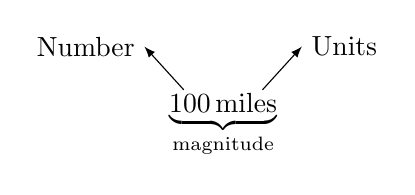
\begin{tikzpicture}
        \draw (0,0) node {$\underbrace{\SI{100}{miles}}_\mathrm{magnitude}$};
        \draw[->] (-0.5,0.45) -- (-1,1) node[left] {Number};
        \draw[->] (0.5,0.45) -- (1,1) node[right] {Units};
    \end{tikzpicture}
\end{center}

A \textbf{\gls{vector}} is \glsdesc{vector}. Directions include north (N), south (S), east (E), west (W), up, left, forward, etc. Examples of vectors include a displacement of \SI{5}{m} N, a velocity of \SI{14}{m/s} to the right, and a momentum of \SI{6}{kg\cdot m/s} forward. Vector notation is shown below.

\begin{center}
    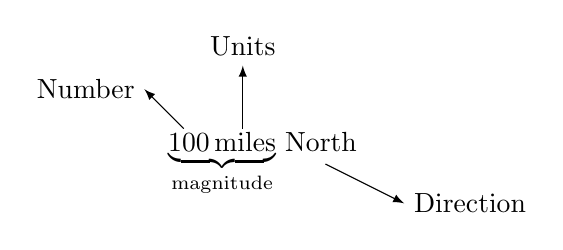
\begin{tikzpicture}
        \draw (0,0) node {$\underbrace{\SI{100}{miles}}_\mathrm{magnitude}$ North};
        \draw[->] (-1,0.45) -- ++(-0.5,0.5) node[left] {Number};
        \draw[->] (-0.25,0.45) -- ++(0,0.8) node[above] {Units};
        \draw[->] (0.8,0) -- ++(1,-0.5) node[right] {Direction};
    \end{tikzpicture}
\end{center}


A vector is drawn as an arrow. The length of the arrow is the magnitude, and the arrowhead is the direction. The \textbf{\gls{tail}} is the \glsdesc{tail}, and the \textbf{\gls{head}} is the \glsdesc{head}.

\begin{center}
    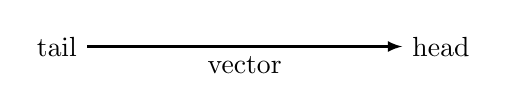
\begin{tikzpicture}
        \draw[->,thick] (0,0) node[left] {tail} -- (4,0) node[right] {head} node[below,pos=0.5] {vector};
    \end{tikzpicture}
\end{center}

The \textbf{\gls{head-to-tail method}} is \glsdesc{head-to-tail method}.

\begin{example}
    Vector $\vec{A}$ is 4 units to the right. Vector $\vec{B}$ is 3 units to the right, as shown below. Add vectors $\vec{A}$ and $\vec{B}$.

\begin{center}
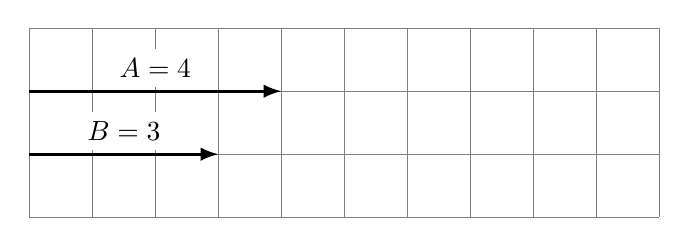
\begin{tikzpicture}[x=8mm,y=8mm]
    \draw[step=8mm,gray] (0,0) grid (10,3);
    \draw[very thick,->] (0,2) -- ++(4,0) node[above=1pt,pos=0.5,fill=white] {$A = 4$};
    \draw[very thick,->] (0,1) -- ++(3,0) node[above=1pt,pos=0.5,fill=white] {$B = 3$};
\end{tikzpicture}
\end{center}
\end{example}

\textit{Solution:}

First, the vectors are added graphically using the head-to-tail method:

\begin{center}
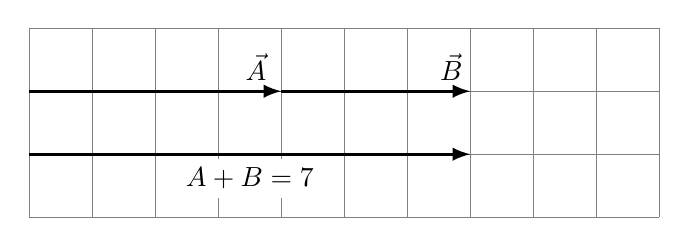
\begin{tikzpicture}[x=8mm,y=8mm]
    \draw[step=8mm,gray] (0,0) grid (10,3);
    \draw[very thick,->] (0,2) -- ++(4,0) node[above,pos=0.9] {$\vec{A}$};
    \draw[very thick,->] (0,2) ++(4,0) -- ++(3,0) node[above,pos=0.9] {$\vec{B}$};
    \draw[very thick,->] (0,1) -- ++(7,0) node[fill=white,below=1pt,pos=0.5] {$A + B = 7$};
\end{tikzpicture}
\end{center}

Therefore, the sum is

\begin{equation*}
    A + B = 4 + 3 = 7
\end{equation*}

\hfill $\blacksquare$

\begin{example}
    Vector $\vec{A}$ is 4 units to the right. Vector $\vec{B}$ is 3 units to the left, as shown below. Add vectors $\vec{A}$ and $\vec{B}$.

\begin{center}
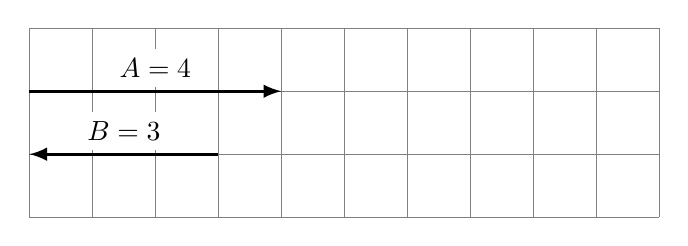
\begin{tikzpicture}[x=8mm,y=8mm]
    \draw[step=8mm,gray] (0,0) grid (10,3);
    \draw[very thick,->] (0,2) -- ++(4,0) node[above=1pt,pos=0.5,fill=white] {$A = 4$};
    \draw[very thick,<-] (0,1) -- ++(3,0) node[above=1pt,pos=0.5,fill=white] {$B = 3$};
\end{tikzpicture}
\end{center}
\end{example}

\textit{Solution:}

The vectors are added graphically using the head-to-tail method:

\begin{center}
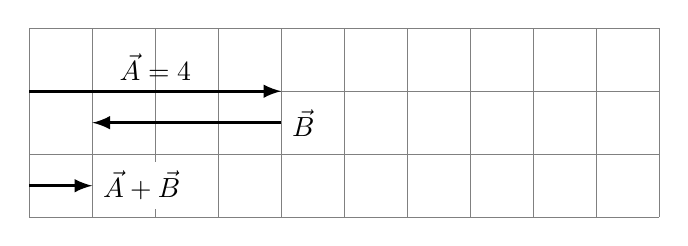
\begin{tikzpicture}[x=8mm,y=8mm]
    \draw[step=8mm,gray] (0,0) grid (10,3);
    \draw[very thick,->] (0,2) -- ++(4,0) node[above,pos=0.5] {$\vec{A} = 4$};
    \draw[very thick,->,yshift=-4mm] (4,2) node[right] {$\vec{B}$} -- ++(-3,0) ;
    \draw[very thick,->] (0,0.5) -- ++(1,0) node[fill=white,right] {$\vec{A} + \vec{B}$};
\end{tikzpicture}
\end{center}

Since $\vec{B}$ points to the left, we subtract its magnitude to find the vector addtion:

\begin{equation*}
    A - B = 4 - 3 = 1
\end{equation*}

Therefore the vector sum is 1 unit to the right.

\hfill $\blacksquare$


Example 3 (You do):

\begin{center}
    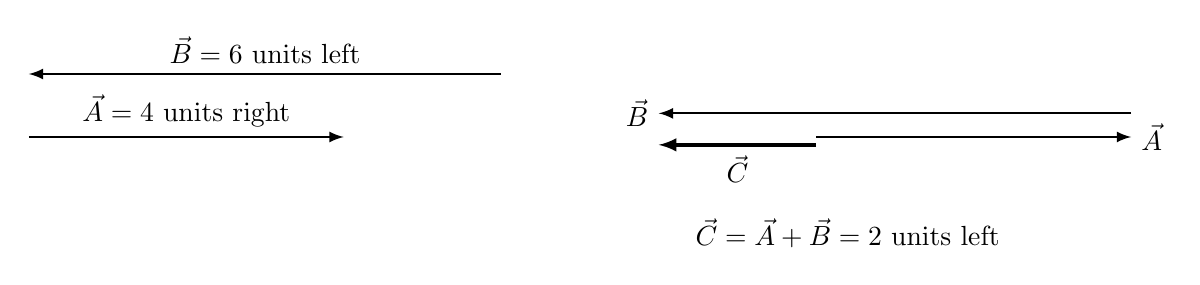
\begin{tikzpicture}
        \draw[->,thick] (0,0) -- (4,0) node[above,pos=0.5] {$\vec{A} = \text{4 units right}$};
        \draw[<-,thick] (0,0.8) -- ++(6,0) node[above,pos=0.5] {$\vec{B} = \text{6 units left}$};
        \begin{scope}[xshift=10cm]
            \draw[->,thick] (0,0) -- (4,0) node[right] {$\vec{A}$};
            \draw[->,thick] (4,0.3) -- ++(-6,0) node[left] {$\vec{B}$};
            \draw[->,very thick] (0,-0.1) -- ++(-2,0) node[below,pos=0.5] {$\vec{C}$} node[below=0.8cm,pos=-0.2] {$\vec{C} = \vec{A} + \vec{B} = \text{2 units left}$};
        \end{scope}
    \end{tikzpicture}
\end{center}

\textbf{\Gls{position}} ($x$) is \glsdesc{position}. The mathematical symbol for position is $x$, and the base SI unit of position is the meter (m). The basic coordinate system for position is a number line called a position axis:

\begin{center}
    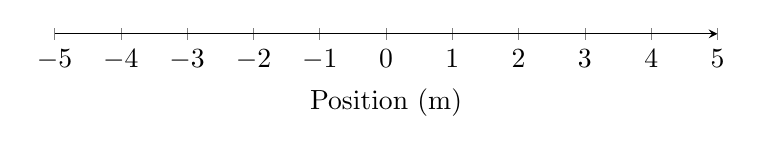
\begin{tikzpicture}
    \begin{axis}[width=10cm,
        axis lines = left,
        axis y line=none,
        xlabel = {Position (m)},
        ymin=0, ymax=1, 
        xmin=-5, xmax=5,
        xtick={-5,-2,...,5},
        clip=false,
        xtick={-5,-4,...,5}
        ]
    \end{axis}
    \end{tikzpicture}
\end{center}

The position of an object may be stated, for example, as $x = \SI{2}{meters}$ or $x = \SI{-3}{m}$. A \textbf{reference point} is a known location used to describe the position of objects, like the zero of a number line.

\begin{example} \label{T7uFg}
A man starts at a reference point, labeled as Point A below. Then he walks to Point B. 

\begin{center}
    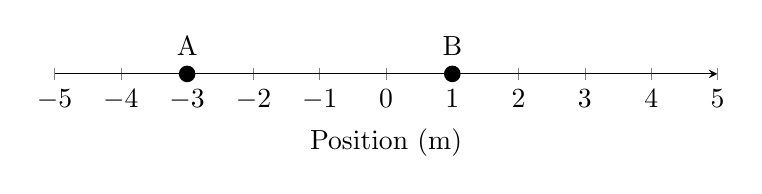
\begin{tikzpicture}
    \begin{axis}[width=10cm,
        axis lines = left,
        axis y line=none,
        xlabel = {Position (m)},
        ymin=0, ymax=1, 
        xmin=-5, xmax=5,
        xtick={-5,-2,...,5},
        clip=false,
        xtick={-5,-4,...,5}
        ]
        \fill (-3,0) circle (3pt) node[above=3pt] {A};
        \fill (1,0) circle (3pt) node[above=3pt] {B};
    \end{axis}
    \end{tikzpicture}
\end{center}

(a) In what direction did his position change? (b) What is the magnitude of the change in his position?
\end{example}

\textit{Solution:}

(a) The man moves to the right, so his position changed in the rightward direction. We can also say it changed in the positive direction.

(b) Recall that magnitude means \glsdesc{magnitude}. We can find change in position by subtracting the first position from the second, exactly the way we do on a number line:

\vspace{-1em}
\begin{align*}
    \text{change in position} &= \SI{1}{m} - \left(-\SI{3}{m}\right) \\[1ex]
    &= \SI{1}{m} + \SI{3}{m} \\[1ex]
    &= \boxed{\SI{4}{m}}
\end{align*}

The man's change in position has a magnitude (size) of 4 meters. That is the same value we would get if we count the tick marks from Point A to Point B.

\hfill $\blacksquare$

The ``change in position'' we just saw in Example \ref{T7uFg} has a special name in physics. \textbf{\Gls{displacement}} ($\Delta x$) is \glsdesc{displacement}. Mathematically, it's

\begin{equation}
    \Delta x = x_f - x_i
\end{equation}

where $x_f$ is the final position $x_i$ is the initial position.


\textbf{\Gls{distance}} ($d$) is \glsdesc{distance}.

Example (I do): Ron Farr runs the following route in 10 seconds: 30 meters in the positive direction, 50 meters in the negative direction, and 15 meters in the positive direction. 

a) What is the distance Ron ran?

Solution: Start by drawing a picture:

\begin{center}
    \begin{tikzpicture}
    \begin{axis}[width=15cm,
        axis lines = left,
        axis y line=none,
        xlabel = {Position (m)},
        ymin=0, ymax=14, 
        xmin=-25, xmax=35,
        % xtick={-5,0},
        % xticklabel={1,2},
        xtick=\empty,
        extra x ticks ={-5,0},
        extra x tick labels={$x_\mathrm{end}=\ ?$,0},
        %xticklabel={$x_\mathrm{end} =\ ?$,0},
        clip=false,
        ]
        \node[above] at (0,0) {\Strichmaxerl[2.5]};
        \draw[thick,->] (0,1) -- ++(axis direction cs: 30,0) node[above,pos=0.5] {30\,m};
        \draw[thick,->] (30,2) -- ++(axis direction cs: -50,0) node[above,pos=0.5] {50\,m};
        \draw[thick,->] (-20,3) -- ++(axis direction cs: 15,0) node[above,pos=0.5] {15\,m};
    \end{axis}
    \end{tikzpicture}
\end{center}

\begin{equation*}
    d = \SI{30}{m} + \SI{50}{m} + \SI{15}{m} = \boxed{\SI{95}{m}}
\end{equation*}

b) What is Ron's displacement?

From the graph above,

\begin{equation*}
    \Delta x = 30 - 50 + 15 = \boxed{\SI{-5}{m}}
\end{equation*}

c) What is his average speed?

\begin{equation*}
    \text{speed} = \frac{\text{distance}}{\text{time}} = \frac{\SI{95}{m}}{\SI{10}{s}} = \boxed{\SI{9.5}{m/s}}
\end{equation*}

d) What is his average velocity?

\begin{equation*}
    v = \frac{\text{displacement}}{\text{time}} = \frac{\SI{-5}{m}}{\SI{10}{s}} = \boxed{\SI{-0.5}{m/s}}
\end{equation*}

\subsubsection{Displacement from a Reference Point}

\subsubsection{Position and Displacements using Multiple Representations}

A \textbf{\gls{position vs. time graph}} is \glsdesc{position vs. time graph}. It shows an object's position at a range of times. For example, 

\begin{center}
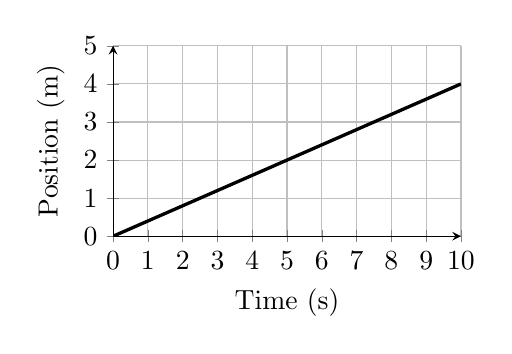
\begin{tikzpicture}
    \begin{axis}[height=4cm,width=6cm,
        axis lines=left,
        ymin=0, ymax=5,
        xmin=0, xmax=10,
        ylabel = {Position (m)},
        xlabel = {Time (s)},
        grid = both,
        ytick={0,1,...,5},
        xtick={0,1,...,10},
    ]
    \addplot[black,very thick,domain=0:10] {2/5*x}; 
\end{axis}
\end{tikzpicture}
\end{center}

The graph above shows that the car traveled 2 meters in 5 seconds, and 4 meters in 10 seconds. In a position vs. time graph, we know where the car is at any time. This graph is one of the ten Multiple Representations.



\begin{example}
The graph below shows the position of an object as a function of time. What is the object's displacement between $t = \SI{2}{s}$ and $t = \SI{5}{s}$?

\begin{center}
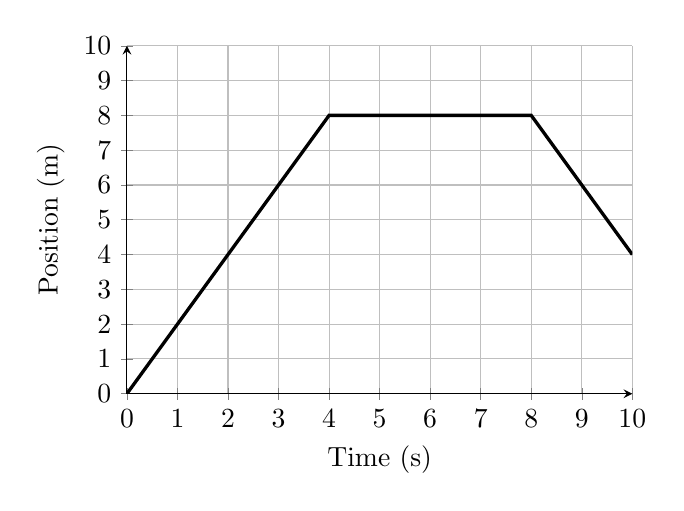
\begin{tikzpicture}
    \begin{axis}[width=8cm,height=6cm,
        axis lines=left,
        ymin=0, ymax=10,
        xmin=0, xmax=10,
        ylabel = {Position (m)},
        xlabel = {Time (s)},
        grid = both,
        xtick={0,1,...,10},
        ytick={0,1,...,10},
    ]
    \addplot[black,very thick]
        coordinates{(0,0)(4,8)(8,8)(10,4)};
\end{axis}
\end{tikzpicture}
\end{center}
\end{example}

\textit{Solution:}

According to the graph, the position of the object at 2 seconds is 4 meters; this is the initial position: $x_i = \SI{4}{m}$. The position at 5 seconds, the final position, is 8 meters: $x_f = \SI{8}{m}$. Displacement is

\begin{equation*}
    \Delta x = x_f - x_i = \SI{8}{m} - \SI{4}{m} = \boxed{\SI{4}{m}}
\end{equation*}

\hfill $\blacksquare$

\subsection{How Fast}

\subsubsection{Velocity and Vectors}

\textbf{\Gls{speed}} is \glsdesc{speed}. It's how hast an object is moving. Mathematically, we can define \textbf{\gls{average speed}} as \glsdesc{average speed}. In equation form,

\begin{equation}
    \text{average speed} = \frac{\mathrm{distance}}{\mathrm{time}}
\end{equation}

The SI units of distance and time are meters and seconds, so the SI units of speed are meters per second~(m/s).

\textbf{\Gls{velocity}} ($v$) is \glsdesc{velocity}, or the rate at which an object changes position. \textbf{\Gls{average velocity}} ($\bar{v}$) is \glsdesc{average velocity}. Mathematically, 

\begin{equation}
    \bar{v} = \frac{\Delta x}{\Delta t} = \frac{\mathrm{displacement}}{\mathrm{time}}
\end{equation}

\subsubsection{Calculating the Velocity of an Object}

\subsubsection{Speed and Velocity using Multiple Representations}

A \textbf{\gls{velocity vs. time graph}} is \glsdesc{velocity vs. time graph}.

\begin{center}
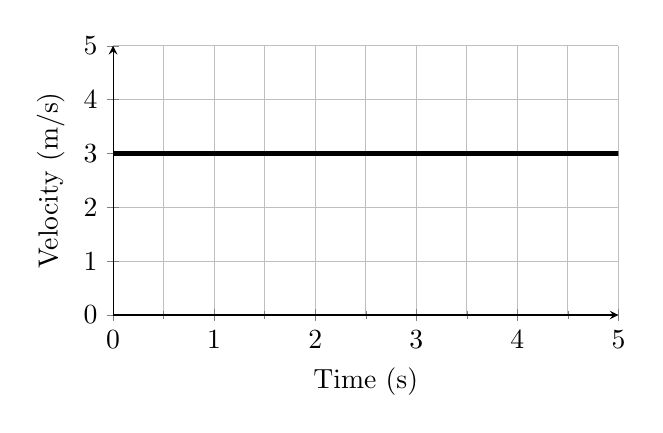
\begin{tikzpicture}
    \begin{axis}[width=8cm,height=5cm,
        axis lines=left,
        ymin=0, ymax=5,
        xmin=0, xmax=5,
        ylabel = {Velocity (m/s)},
        xlabel = {Time (s)},
        grid = both,
        xtick={0,1,...,10},
        ytick={0,1,...,5},
        minor x tick num=1,
    ]
    \addplot[ultra thick,domain=0:10] plot {3};
\end{axis}
\end{tikzpicture}
\end{center}

\subsubsection{Predicting Displacement and Velocity}

\subsubsection{Constant Motion using Multiple Representations}

\subsubsection{Displacement from a Position vs. Time and Velocity vs. Graph}

\subsection{Mass and Inertia}

\subsubsection{Defining Inertia and Mass}

\textbf{\Gls{inertia}} is \glsdesc{inertia}. \textbf{\Gls{mass}} is \glsdesc{mass} (kg). Inertia is proportional to mass: the more mass an object has, the greater its inertia. 

\textbf{\gls{Newton's first law of motion}} states that \glsdesc{Newton's first law of motion}.

% [Begin with several demos of inertia without using the word ``inertia.''

% \begin{enumerate}[itemsep=0pt,topsep=0pt]
%     \item Stand a roll of painter's tape on the rim of a flask. Place penny on top of roll. Forcefully pull roll from under the penny and watch the penny land inside the flask.
%     \item Place a stack of heavy textbooks on a cart. Place a light object (e.g. whiteboard eraser) on top of books. ``Crash'' the cart on a table and watch the eraser fly onto the table top away from the cart.
%     \item In the middle of the night on March 26, 2024,  a cargo ship on a river near Baltimore lost all power and crashed into a bridge, killing 6 people.
%     \item The sleeping Pokemon snorlax could not be removed from the edge of a creek.
%     \item Messi (\href{https://www.youtube.com/watch?v=5PKXs8i_zSw&t=19s}{click here})
%     \item Football (\href{https://www.youtube.com/watch?v=4TgpW0WZZ6U&t=55s}{click here})
%     \item Basketball (\href{https://www.youtube.com/watch?v=IGBpvIXGMYQ&t=24s}{click here})
%     \item Snowboard girl chased by a bear (\href{https://www.youtube.com/watch?v=vT_PNKg3v7s}{click here})
% \end{enumerate}

% Give students large paper and ask them to brainstorm: What do all these things have in common?
% ]


\subsubsection{Relating Inertia to Mass}

\clearpage

\subsection{Momentum}

\subsubsection{Differentiating between Inertia and Momentum}

\textbf{\Gls{momentum}} ($p$) is \glsdesc{momentum}. Mathematically, 

\begin{equation*}
    p = mv
\end{equation*}

The SI unit of momentum is the combination of the units of mass and velocity: kilograms multiplied by meters per second, or $\mathrm{kg\cdot m/s}$. Objects usually don't change in mass but can change momentum with change in velocity. 

\subsubsection{Momentum using Multiple Representations}

A \textbf{\gls{momentum vs. time graph}} is \glsdesc{momentum vs. time graph}.

\begin{center}
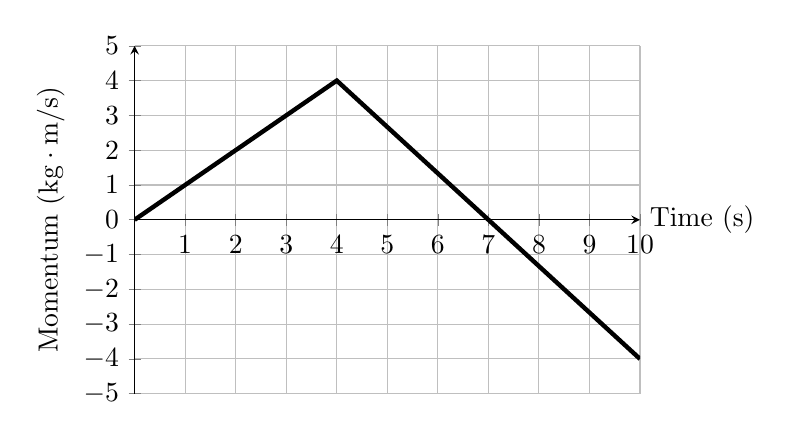
\begin{tikzpicture}
    \begin{axis}[width=8cm,height=6cm,
        axis y line=left,
        axis x line=center,
        ymin=-5, ymax=5,
        xmin=0, xmax=10,
        ylabel = {Momentum ($\mathrm{kg\cdot m/s}$)},
        xlabel = {Time (s)},
        grid = both,
        ytick={-5,-4,...,5},
        xtick={0,1,...,10},
        x label style={at={(axis description cs: 1,0.5)},anchor=west}
    ]
    \addplot[ultra thick,domain=0:10] plot coordinates {(0,0)(4,4)(10,-4)};
\end{axis}
\end{tikzpicture}
\end{center}


\subsubsection{Calculating Momentum}

\subsection{Kinetic Energy}

\subsubsection{Differentiating between Momentum and Kinetic Energy}

% [Watch Chris Farley on the Letterman show (\href{https://youtu.be/Nzl2lvO1aMs?feature=shared&t=101}{CLICK HERE}). Then fill in the blank below. On a sticky note, students fill in the blank in the following sentence: 

% \begin{center}
%   Chris Farley has a lot of \rule{4cm}{0.15mm}\ .  
% \end{center}

% ]

\textbf{\Gls{kinetic energy}} (KE) is \glsdesc{kinetic energy}. Mathematically, it's defined as

\begin{equation*}
    \mathrm{KE} = \frac{1}{2} m v^2
\end{equation*}

where $m$ is mass in kilograms and $v$ is speed in meters per second. According to this equation, since the SI base units of mass and velocity are the kilogram and the meter per second, respectively, kinetic energy has units of

\begin{equation*}
    \mathrm{kg} \cdot \left(\mathrm{\frac{m}{s}}\right)^2 = \mathrm{\frac{kg\cdot m^2}{s^2}}
\end{equation*}

This combination of kg, m, and s has a special name: the joule. A \textbf{\gls{joule}} (J) is \glsdesc{joule}:

\begin{equation*}
    \SI{1}{J} = 1\,\mathrm{\frac{kg\cdot m^2}{s^2}}
\end{equation*}

``Work'' is a physics concept that will be introduced in Unit 4.

\begin{example}
A 250-gram cart travels at 3.2 meters per second. Calculate its kinetic energy. 
\end{example}

\textit{Solution:}

$m = \SI{0.25}{kg}$ and $v = \SI{1.5}{m/s}$. $\mathrm{KE} =\ ?$

\begin{equation*}
    \mathrm{KE} = \frac{1}{2} mv^2 = \frac{1}{2}(\SI{0.25}{kg})(\SI{1.5}{m/s})^2 = \boxed{\SI{1.28}{J}} 
\end{equation*}

\hfill $\blacksquare$

\subsubsection{Comparing Kinetic Energies of Different Objects}

\subsubsection{Calculating Kinetic Energy}

\subsection{Frame of Reference}

\subsubsection{Relative Motion}

\subsubsection{Calculating Relative Velocity}

Hook: ``The Fast and the Furious'' (\href{https://youtu.be/yWiSjVHCT30?feature=shared&t=238}{click here}). Look at the velocity of the red car relative to the green car towards the end of the race.

% \textbf{Frame of Reference}: the point of view from which we look at a motion.

Examples of a frame of reference are:

\begin{itemize}[itemsep=0pt,topsep=0pt]
    \item Person sitting in a car
    \item Person looking at the car from the sidewalk
    \item Person riding a bike in the opposite direction
\end{itemize}

\textbf{Relative speed} is how fast or slow an object appears to be moving to another object.

% When objects move together: add their velocities

% When objects move apart: subtract their velocities.


\fi

\clearpage

\section{Force Interactions}

\ifShowUnitII
\setcounter{example}{0}

\subsection{Interacting Objects}

\subsubsection{Types of Force}

A \textbf{\gls{force}} is \glsdesc{force}. Being vectors, forces are represented by arrows. The length of the arrow is the magnitude of the force. For example, force $\vec{F}_1$ below has a magnitude of 5 newtons, and the magnitude of $\vec{F}_2$ is \SI{8}{N}.

\begin{center}
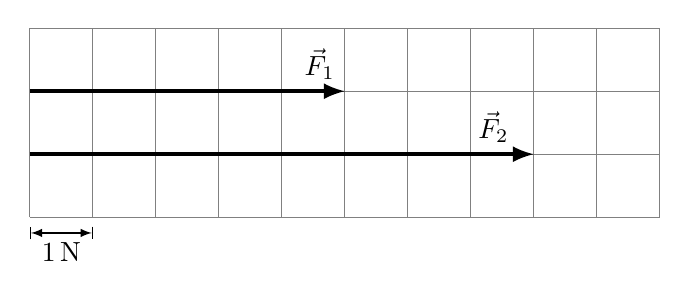
\begin{tikzpicture}[x=8mm,y=8mm]
    \draw[step=8mm,gray] (0,0) grid (10,3);
    \draw[ultra thick,->] (0,2) -- ++(5,0) node[above,pos=0.92] {$\vec{F}_1$};
    \draw[ultra thick,->] (0,1) -- ++(8,0) node[above,pos=0.92] {$\vec{F}_2$};
    \draw[|<->|,yshift=-2mm] (0,0) -- (1,0) node[below,pos=0.5] {\SI{1}{N}}; 
\end{tikzpicture}
\end{center}

In this unit, there are six forces you should know: the gravitational force, the normal force, the frictional force, the applied force, the spring force, and tension.


The \textbf{\gls{gravitational force}} ($F_g$) is \glsdesc{gravitational force}. In the case below, there is a force of gravity on the ball. 

\begin{center}
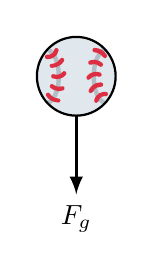
\begin{tikzpicture}
    \draw[very thick,->] (0,0) -- (0,-1.5) node[below] {$F_g$};
    \node at (0,0) {\twemoji[width=1cm]{baseball}};
    \draw[thick] (0,0) circle (0.5);
\end{tikzpicture}
\end{center}

Where does the force $F_\mathrm{g}$ come from? It comes from Earth, which gravitationally pulls the ball down. The gravitational force will be explore in more detail in Unit 5.

A \textbf{\gls{normal force}} ($F_\text{N}$) is \glsdesc{normal force}. In the case of a baseball, if the ball is rested on a flat surface like a bed, the normal force is the upward force exerted by the bed on the ball:

\begin{center}
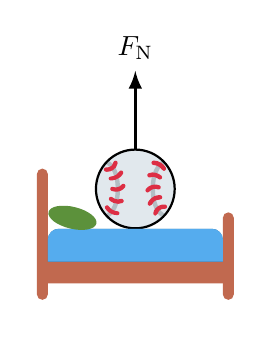
\begin{tikzpicture}
    \draw[very thick,->] (0,0) -- (0,1.5) node[above] {$F_\mathrm{N}$};
    \node at (0,0) {\twemoji[width=1cm]{baseball}};
    \draw[thick] (0,0) circle (0.5);
    \node[yshift=-4.5pt] at (0,0) {\twemoji[width=2.5cm]{1f6cf}};
\end{tikzpicture}
\end{center}


The \textbf{\gls{frictional force}} ($F_f$) is \glsdesc{frictional force}. An \textbf{\gls{applied force}} ($F_\mathrm{A}$) is \glsdesc{applied force}. In the example below, if a box is resting on a rough surface and an applied force moves it to the right with constant motion, then there is a frictional force in the opposite direction.

\begin{center}
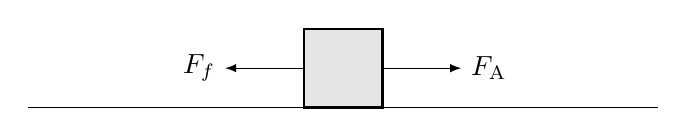
\begin{tikzpicture}
    \draw (-2,0) -- (6,0);
    % \draw[->] (2,0.5) -- ++(0,+1.3) node[above] {$F_\mathrm{N}$};
    % \draw[->] (2,0.5) -- ++(0,-1.3) node[below] {$F_g$};
    \draw[->] (2,0.5) -- ++(+1.5,0) node[right] {$F_\mathrm{A}$};
    \draw[->] (2,0.5) -- ++(-1.5,0) node[left] {$F_f$};
    \draw[thick,fill=black!10] (1.5,0) rectangle ++(1,1);
\end{tikzpicture}
\end{center}

The \textbf{\gls{spring force}} ($F_s$) is \glsdesc{spring force}. If an object is suspended from a spring, the spring applies an upward force to sustain the object's weight.

\begin{center}
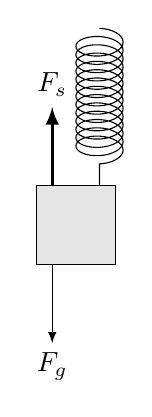
\begin{tikzpicture}
    \draw[decorate,decoration={coil,segment length=3pt,post length=2mm,pre length=0mm,amplitude=3mm}] (0,0) -- ++(0,-2);
    \begin{scope}[shift={(-0.8,-3)}]
        \draw[very thick,->] (0.2,0) -- ++(0,2) node[above] {$F_s$};
        \draw[fill=black!10] (0,0) rectangle (1,1);
        \draw[->] (0.2,0) -- ++(0,-1) node[below] {$F_g$};
    \end{scope}
\end{tikzpicture}
\end{center}

\textbf{\Gls{tension}} ($F_\mathrm{T}$) is \glsdesc{tension}.

One example of tension is tetherball, the sport where a ball is connect by a rope to a stationary pole:

\begin{center}
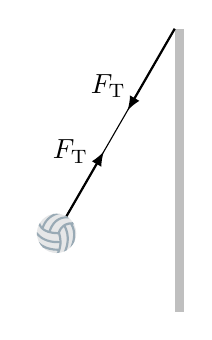
\begin{tikzpicture}[x=1.2cm,y=1.2cm]
    \fill[lightgray] (0,0) rectangle (0.1,3);
    \begin{scope}[shift={(0,3)}]
        \draw (0,0) -- ({-2.5*cos(60)},{-2.5*sin(60)});
        \draw[thick,->] (0,0) -- ({-cos(60)},{-sin(60)}) node[left=2pt,pos=0.7] {$F_\mathrm{T}$};
        \draw[thick,->] ({-2.5*cos(60)},{-2.5*sin(60)}) -- ++({cos(60)},{sin(60)}) node[left=2pt] {$F_\mathrm{T}$};
        \node at ({-2.5*cos(60)},{-2.5*sin(60)}) {\twemoji[width=5mm]{volleyball}};
    \end{scope}   
\end{tikzpicture}
\end{center}

When the rope is taught, there is a tension force on the ball, and another tension force of equal magnitude is exerted on the pole, to keep the ball in motion.

\subsubsection{Representing Force Pairs in Interactions}

Let $F_\text{box-table}$ be the force on the box by the table, and $F_\text{table-box}$ be the force on the box by the table. In general, $F_\text{A-B}$ is the force on object A by object B. 

$F_\text{box-table}$ is a reaction to the action of $F_\text{table-box}$. They have the same magnitude but opposite directions.

We call $F_\text{box-table}$ and $F_\text{table-box}$ force pairs.


\begin{center}
    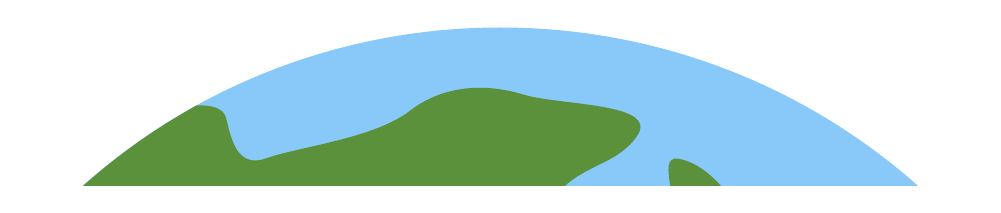
\begin{tikzpicture}
        \clip (-6,6) rectangle ++(12,2);    
        \node at (0,0) {\twemoji[width=16cm]{globe showing Americas}};  
    \end{tikzpicture}
\end{center}


\begin{center}
    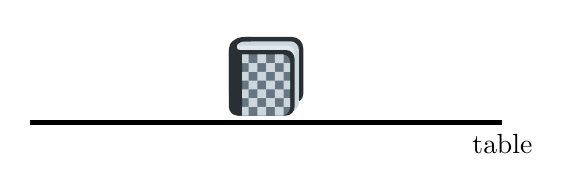
\begin{tikzpicture}
        \draw (0,0) node[above=-1pt] {\twemoji[height=1cm]{notebook}};
        \draw[ultra thick] (-3,0) -- ++(6,0) node[below] {table};
    \end{tikzpicture}
\end{center}

Let $F_\text{book-table}$ by the force on the book by the table; $F_\text{table-book}$, the force on the table by the book, etc.

\begin{center}
    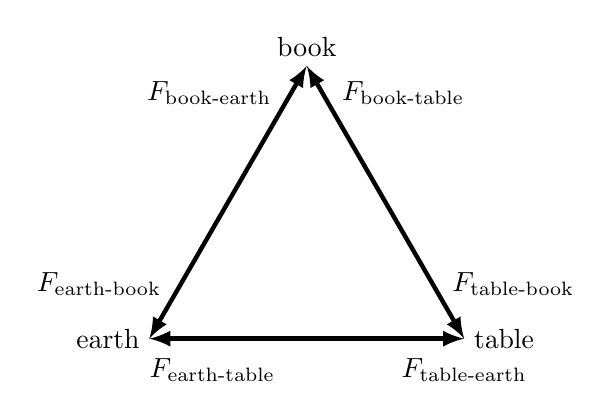
\begin{tikzpicture}
        \coordinate (earth) at (0,0); 
        \coordinate (table) at ({4},0); 
        \coordinate (book) at ({4*cos(60)},{4*sin(60)}); 
        \draw (book) node[above] {book};
        \draw (table) node[right] {table};
        \draw (earth) node[left] {earth};
        \draw[ultra thick,<->] (book)  -- (table) node[right=3pt,pos=0.1] {$F_\text{book-table}$} node[right=3pt,pos=0.8] {$F_\text{table-book}$};
        \draw[ultra thick,<->] (book) -- (earth) node[left=3pt,pos=0.1] {$F_\text{book-earth}$} node[left=3pt,pos=0.8] {$F_\text{earth-book}$};
        \draw[ultra thick,<->] (earth) -- (table) node[below=3pt,pos=0.2] {$F_\text{earth-table}$} node[below=3pt] {$F_\text{table-earth}$} ;
    \end{tikzpicture}
\end{center}

An object can be involved in multiple force interactions.

Any one interaction is between two objects and involves two forces.

Newton's action-reaction law: ``For every action, there is an equal but opposite reaction.''

Forces always come in pairs.

Each force in a force pair is the same magnitude (size or strength) but acts in opposite directions.

The force on the book from the table (FBT) is equal  to the force on the table from the book (FTB) but the book pushes down on the table and the table pushes up on the book. Equal but opposite.

The force on the book from the table (FBE) is equal  to the force on the table from the book (FEB) but the book pushes down on the table and the table pushes up on the book. Equal but opposite.

The force on the book from the table (FTE ) is equal  to the force on the table from the book (FET) but the book pushes down on the table and the table pushes up on the book. Equal but opposite.

\subsubsection{Force Pairs as Two Forces of the Same Type}

\subsubsection{Instances in which Forces are Not a Force Pair}

\subsection{Constant Motion Model Based on Forces}

\subsubsection{Free-Body Diagrams}

A \textbf{\gls{free body diagram}} is \glsdesc{free body diagram}. They are a tool for analyzing net force and predicting motion. A free body diagram is focused on one object only and shows a moment in time. It includes the forces acting \textit{on} the object but no forces \textit{by} the object. It consists of a dot with arrows (force vectors) coming off the object for every force interaction, as shown below.

\begin{center}
\begin{tikzpicture}[x=1.2cm,y=1.2cm]
    \draw[->,thick] (0,0) -- (1,0) node[right] {$F$};
    \draw[->,thick] (0,0) -- (-1,0) node[left] {$F_f$};
    \draw[->,thick] (0,0) -- (0,1) node[above] {$F_\text{N}$};
    \draw[->,thick] (0,0) -- (0,-1) node[below] {$F_g$};
    \fill (0,0) circle (4pt);
\end{tikzpicture}
\end{center}

\subsubsection{Effects of Balanced and Unbalanced Forces}

\subsubsection{Multiple Representations for Constant and Changing Velocity, Momentum, Kinetic Energy, and Forces}

% \begin{example}
% What is the weight of a 12\,kg box?
% \end{example}

% \textit{Solution:}

% Answer: $w = mg = (\SI{12}{kg})(\SI{10}{m/s^2}) = \SI{120}{N}$

% \hfill $\blacksquare$

% \begin{example}
% A 3\,kg book rests on a table. Find the normal force.
% \end{example}

% \begin{center}
% \begin{tikzpicture}
%     \draw[fill=black!20] (0,0) rectangle ++(4,0.4);
%     \draw[fill=black!20] (0.5,0) rectangle ++(0.2,-2);
%     \draw[fill=black!20] (3.3,0) rectangle ++(0.2,-2);
%     \node[above=2.9mm] at (2,0) {\twemoji[height=1cm]{blue book}};
% \end{tikzpicture}
% \end{center}

% Recall: Normal force is the perpendicular force that an surface exerts to support the weight of an object. 

% Normal force is equal in magnitude to weight, opposite in direction

% Weight is

% \begin{equation*}
%     w = mg = (\SI{3}{kg})(\SI{10}{m/s^2}) = \SI{30}{N} \quad \text{down}
% \end{equation*}

% Magnitude of the normal force is

% \begin{equation}
%     F_\mathrm{n} = \left|w\right| = \SI{30}{N}
% \end{equation}

% and the direction is up.

% \hfill $\blacksquare$

\fi

\clearpage

\section{The Law of Acceleration}

\ifShowUnitIII
\setcounter{example}{0}

\subsection{Acceleration}

\subsubsection{The Concept of Acceleration}

\textbf{\Gls{acceleration}} ($a$) is \glsdesc{acceleration}. Mathematically, \textbf{\gls{average acceleration}} is \gls{average acceleration}:

\begin{equation*}
    a = \frac{\Delta v}{\Delta t} = \frac{v_f - v_i}{\Delta t}
\end{equation*}

One of the best ways to study acceleration is to look at data, both quantitative and qualitative. 

\subsubsection{Zero Acceleration, Positive Acceleration, and Negative Acceleration}

\subsubsection{Comparing Accelerations of Objects}

\subsubsection{Determining Change in Velocity and Acceleration from Multiple Representations}

\begin{example}
The graph below shows the velocities of Car A and Car B as a function of time. Describe the acceleration of each car.

\begin{center}
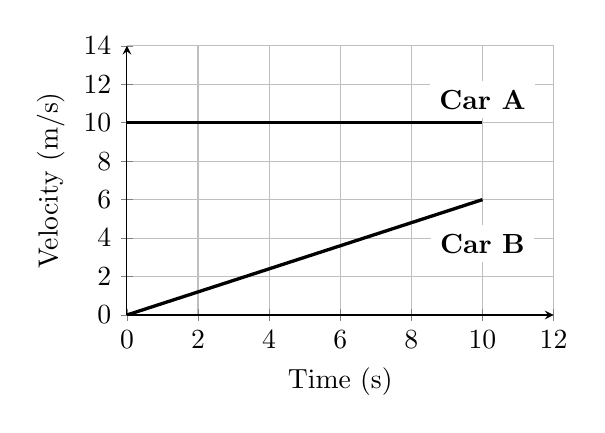
\begin{tikzpicture}
    \begin{axis}[height=5cm,
        width=7cm,
        ylabel={Velocity (m/s)},
        xlabel={Time (s)},
        ymin=0,ymax=14,
        xmin=0,xmax=12,
        ytick={0,2,...,14},
        xtick={0,2,...,12},
        axis lines=left,
        grid=both,
    ]
    \addplot[very thick,black] coordinates{(0,0)(10,6)} node[below=3mm,fill=white] {\textbf{Car B}};
    \addplot[very thick,black] coordinates{(0,10)(10,10)} node[above=1pt,fill=white] {\textbf{Car A}};
    \end{axis}
\end{tikzpicture}    
\end{center}
\end{example}

\textit{Solution:}

Car A has a constant velocity of \SI{10}{m/s}. Since acceleration is a change in velocity over time, this car has an acceleration of zero. In other words, it's not accelerating.

The velocity of Car B starts at zero and increases to \SI{6}{m/s} in 10 seconds. By definition, since velocity is changing, this car \textit{is} accelerating.

\hfill $\blacksquare$

\begin{example}
A toy car in a lab starts from rest and travels 1 meter in the first second. However, it travels a greater distance in the 2nd second, and increasingly longer distances with each passing second, as shown in the table below.

\begin{center}
    \begin{tabular}{|c|c|}
        \hline
         \textbf{Time} (s) & \textbf{Position} (m) \\ \hline
         0 & 0 \\ \hline
         1 & 1 \\ \hline
         2 & 4 \\ \hline
         3 & 9 \\ \hline
         4 & 16 \\ \hline
         5 & 25 \\ \hline
    \end{tabular}
\end{center}

A student claims that the car is traveling at a constant velocity. Is the student correct?
\end{example}

\textit{Solution:}

The car's displacement between $t = \SI{0}{s}$ and $t = \SI{1}{s}$ is \SI{1}{m}. The displacement between $t = \SI{1}{s}$ and $t = \SI{2}{s}$ is \SI{3}{m}. The displacement between $t = \SI{2}{s}$ and $t = \SI{3}{s}$ is \SI{5}{m}. And, the last two displacements are \SI{7}{m} and \SI{9}{m}. Because the car is not moving with equal displacements across equal time intervals, the student is wrong, the object's velocity is \textit{not} constant but changing, and therefore the car is accelerating.

\hfill $\blacksquare$

\subsubsection{Representations of Changing Motion}

\subsubsection{Predicting Change in Velocity and Acceleration using Number Sense}

\subsection{Newton's Law of Acceleration}

\subsubsection{The Relationship between Net Force and Acceleration}

\textbf{\Gls{net force}} ($F_\text{net}$) is \glsdesc{net force}. Mathematically, it can be related to acceleration as

\begin{equation*}
    F_\text{net} = ma
\end{equation*}


\begin{example}
In a game of tug of war, Blue Team applies a 300-newton force to the left, and Red Team applies a 350\,N force to the right. Calculate the net force. Assume the positive direction is to the right.
\end{example}

\textit{Solution:} 

Taking rightward to be the positive direction, the net force is given by

\begin{equation*}
    F_\mathrm{net} = F_\mathrm{red} - F_\mathrm{blue} = \SI{350}{N} - \SI{300}{N} = \boxed{+\SI{50}{N}}
\end{equation*}

or 50 newtons to the right.

\hfill $\blacksquare$


\begin{example}
From the previous example, Team Blue acquires a new strong player who applies an additional 150\,N force. What is the net force now?
\end{example}

\textit{Solution:}

\begin{equation*}
    F_\mathrm{net} = F_\mathrm{red} - F_\mathrm{blue} = \SI{350}{N} - \SI{450}{N} = \boxed{-\SI{100}{N}}
\end{equation*}

or 100 newtons to the left.

\hfill $\blacksquare$

\subsubsection{The Relationship between Mass and Acceleration}

\subsubsection{The Effects of Changing Net Force on Mass or Acceleration}

\subsubsection{Solving Problems using Newton's Second Law}

\clearpage

\fi

\section{Impulse and Work}

\ifShowUnitIV
\setcounter{example}{0}

\subsection{Changing Momentum}

\subsubsection{Relating Change in Momentum to Change in Velocity}

Recall that momentum is
 
\begin{equation*}
    p = m v
\end{equation*}

and its units are \SI{}{kg\cdot m/s}. Change in an object's momentum is 

\begin{equation*}
    \Delta p = p_f - p_i
\end{equation*}

where $p_f$ is final momentum and $p_i$ is initial momentum. Assuming an object's mass does not change, then an object changes momentum if it changes velocity:

\begin{equation*}
    \Delta p = m \Delta v = m(v_f - v_i)
\end{equation*}

\begin{example}
An \SI{0.080}{kg} egg is drop from rest and reaches a velocity of \SI{4.4}{m/s}. Calculate the egg's change in momentum.
\end{example}

\textit{Solution:}

We know

\vspace{-1em}
\begin{align*}
    m &= \SI{0.08}{kg} \\[1ex]
    v_i &= \SI{0}{m/s} \\[1ex]
    v_f &= \SI{4.4}{m/s} \\[1ex]
\end{align*}

Thus, the change in momentum is

\vspace{-1em}
\begin{align*}
    \Delta p &= m (v_f - v_i) \\[1ex]
    &= (\SI{0.08}{kg})(\SI{4.4}{m/s} - \SI{0}{m/s}) \\[1ex]
    &= \boxed{\SI{0.352}{kg\cdot m/s}}
\end{align*}

\hfill $\blacksquare$

Make a list of all physics key terms we have used since the beginning of the school year. List may include: position, velocity, speed, time, acceleration, momentum, kinetic energy, force, etc. 

\textbf{Example 2}. An egg is dropped from rest and reaches a final velocity of \SI{4.4}{m/s} right before striking a pillow. An identical egg is dropped from the same height and reaches the same final velocity. 

\begin{center}
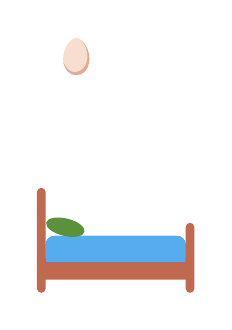
\begin{tikzpicture}
    \node at (0,0) {\twemoji[width=2cm]{1f6cf}};
    \node at (-0.5,2) {\twemoji[height=5mm]{egg}};
\end{tikzpicture}
\hspace{2cm}
\begin{tikzpicture}
    \node at (0,0) {\phantom{\twemoji[width=2cm]{1f6cf}}};
    \node at (-0.5,2) {\twemoji[height=5mm]{egg}};
    \draw (-2,0) -- ++(4,0) node[below,pos=0.5] {concrete floor};
\end{tikzpicture}
\end{center}

The first egg survives the fall while the second egg breaks. Why? Use ideas from the physics terms in the previous activity to arrive at an explanation.

[Transition to the The Egg Drop activity at physicsclassroom.com (\href{https://www.physicsclassroom.com/physics-interactives/momentum-and-collisions/egg-drop/egg-drop-interactive}{CLICK HERE}). Find the spreadsheet in Schoology. Get them started on the spreadsheet, then have them finish it.]



\subsubsection{The Relationship between Net Force and Momentum}

\subsubsection{The Relationship between Time and Momentum}

\textbf{\Gls{impulse}} ($J$) is \glsdesc{impulse}. Mathematically, it is 

\begin{equation*}
    J = F_\text{net} \Delta t
\end{equation*}

The \textbf{\gls{impulse-momentum theorem}} states that \glsdesc{impulse-momentum theorem}.

\begin{equation*}
    F_\text{net} \Delta t = \Delta p
\end{equation*}

Therefore, impulse-momentum theorem is also written as

\begin{equation*}
    F_\text{net} \Delta t = m \Delta v = m(v_f - v_i)
\end{equation*}




\subsubsection{Real-Life Applications of Impulse and Momentum}

\subsubsection{Solving Problems Using the Impulse-Momentum Theorem}

\subsection{Changing Kinetic Energy}

\begin{center}
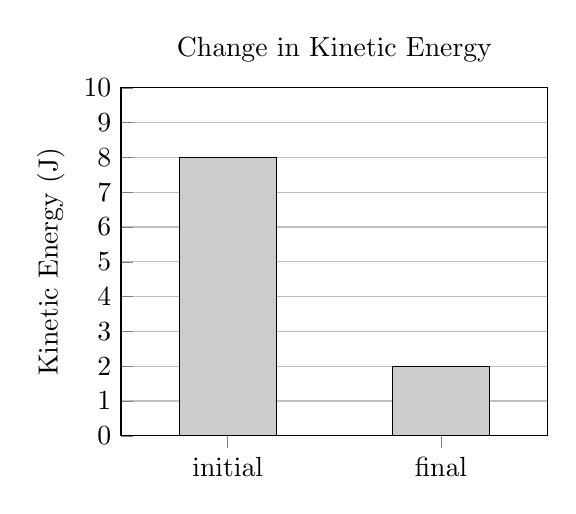
\begin{tikzpicture}
\begin{axis}[width=7cm,height=6cm,
    % axis lines=left,
    ybar,
    symbolic x coords={initial, final},
    xtick=data,
    ylabel={Kinetic Energy (J)},
    ymin=0, ymax=10,
    ytick={0,1,...,10},
    bar width=35pt,
    enlarge x limits=0.5,
    ymajorgrids=true,
    tick pos=left,
    title={Change in Kinetic Energy}
]
\addplot[black,fill=black!20] coordinates {(initial,8) (final,2)};
\end{axis}
\end{tikzpicture}
\end{center}

\textbf{\Gls{work}} is \glsdesc{work}.

\begin{example}
A \SI{12}{N} force is applied on a box, and the box moves a distance of 7 meters. What is the work done on the box?
\end{example}


\textit{Solution:}

\hfill $\blacksquare$

More specifically, work is the component of the force in the direction of the displacement, multiplied by the displacement.

\subsubsection{Identifying if a Net Force is Doing Work}

\subsubsection{Calculating Net Work}

\begin{example} \label{HKavsZ}
Jacob applies a force of \SI{72.0}{N} on a box and pushes it a distance of \SI{25.0}{m}. How much work is done on the box?
\end{example} 

\begin{center}
    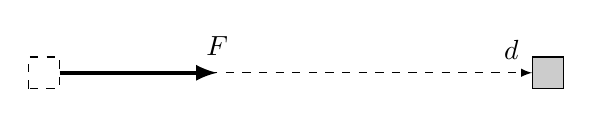
\begin{tikzpicture}
    \begin{scope}[xshift=-4mm,yshift=-2mm]
        \draw[dashed] (0,0) rectangle (4mm,4mm);
    \end{scope}
    \begin{scope}[xshift=6cm,yshift=-2mm]
        \draw[fill=black!20] (0,0) rectangle (4mm,4mm);
    \end{scope}
    \draw[ultra thick, ->] (0,0) -- (2,0) node[above=2pt] {$F$};
    \draw[->, dashed] (0,0) -- (6,0) node[above left=2pt] {$d$};
    \end{tikzpicture}
\end{center}

\textit{Solution:} 

We are given the quantities of force and distance: $F = \SI{72.0}{N}$ and $d = \SI{25.0}{m}$. The unknown quantity we want to find is work. By Equation~(\ref{y0Z6Cw}), 

\begin{equation*}
    W = F d = \left(\SI{72.0}{N}\right)\left(\SI{25.0}{m}\right) = \SI{1800}{J}
\end{equation*}

Jacob does 1800 joules of work on the box in applying the force to move the box.

\hfill $\blacksquare$


\begin{example}\label{O9RxyJ}
You see a box with a mass of \SI{10}{kg} resting on the floor. What is the work you have to do on the box to lift it to a height of 1.5 meters? 
\end{example} 
 

\textit{Solution:} 
We are given the box's mass and distance lifted: $m = \SI{10}{kg}$ and $d = \SI{1.5}{m}$. The unknown we are looking for is work: $W =\ ?$ By Eq.~(\ref{y0Z6Cw}), work is

\begin{equation*}
    W = F d
\end{equation*}

However, force ($F$) is \textit{not} one of the given quantities in this problem. Can you of a way to calculate how much force is necessary to lift this box? To lift the box, you must supply an upward force that is (at least) equal to the magnitude of the downward force of gravity on the box. That is, your applied force must equal the box's weight ($w$), which, in Unit 4 on Forces, we specifically defined as

\begin{equation*}
    w = m g\ ,
\end{equation*}

where  g = \SI{9.8}{m/s^2}. So, if your applied force is equal to the box's weight, then your force is

\begin{equation*}
    F = w = mg = (10)(9.8) = \SI{98}{N}
\end{equation*}

Therefore, the work done is

\begin{equation*}
    W = F d = (\SI{98}{N})(\SI{1.5}{m}) = \SI{147}{J} \ .
\end{equation*}

\textbf{Note}: Since, in this example, the force was of the form $F = mg$ and since work is defined as $W = F d$, the work done against gravity was of the form $W = mgd$. Compare this result with Equation (\ref{RlpJa5}) below.

\hfill $\blacksquare$

\subsubsection{The Relationship between Net Force and Kinetic Energy}

\subsubsection{The Relationship between Displacement and Kinetic Energy}

\subsubsection{Solving Problems using the Work-Energy Theorem}

\subsubsection{Comparing the Power of Various Situations}

\subsubsection{Calculating Power}

\fi

\clearpage

\section{Force Analysis}

\ifShowUnitV
\setcounter{example}{0}

\subsection{Newton's Law of Universal Gravitation}

\subsubsection{The Law of Gravitation}

\textbf{\gls{Newton's universal law of gravitation}} \glsdesc{Newton's universal law of gravitation}.

\begin{center}
    \begin{tikzpicture}[rotate=10]
        \draw (0,0) circle (5mm) node[above=5mm] {$m_1$};
        \draw[|<->|,above=2mm] (0,0) -- (8,0) node[above,pos=0.5] {$r$};
        \draw (8,0) circle (8mm) node[above=8mm] {$m_2$};
        \fill (0,0) circle (2pt);
        \fill (8,0) circle (2pt);
        \draw[thick,->,right=1mm] (0,0) -- (2,0) node[below,pos=0.8] {$F_g$};
        \draw[thick,->,left=1mm] (8,0) -- (6,0) node[below,pos=0.8] {$F_g$};
    \end{tikzpicture}
\end{center}

The magnitude of the gravitational force is

\begin{equation*}
    F_g  = G\frac{m_1 m_2}{r^2}
\end{equation*}

where $G$ is the \textbf{\gls{gravitational constant}}, \glsdesc{gravitational constant}, and is equal to

\begin{equation*}
    G = \SI[per-mode=fraction]{6.67e-11}{\newton\meter\tothe{2}\per\kilogram\tothe{2}}
\end{equation*}

\begin{example}
Consider two spheres of mass \SI{100.0}{kg} and \SI{400.0}{kg} whose centers are separated by \SI{4.00}{m}. What is the magnitude of the gravitational force between them?
\end{example}

\textit{Solution:}
We are given two masses and the distance between them: $m_1 = \SI{100.0}{kg}$, $m_2 = \SI{400}{kg}$, $r = \SI{4.00}{m}$. Also, remember that $G = \SI{6.67e-11}{N\,m^2/kg^2}$. By Newton's law of universal gravitation, the gravitational force is

\begin{equation*}
    F = \frac{G m_1 m_2}{r^2} = 
    \frac{\left(\SI[per-mode=fraction]{6.67e-11}{\newton\meter\tothe{2}\per\kilogram\tothe{2}}\right) (\SI{100}{kg}) (\SI{400}{kg})}{\left(\SI{4.00}{m}\right)^2} = 
    \boxed{\SI{1.67e-7}{N}}
\end{equation*}

\hfill $\blacksquare$



\subsubsection{Comparing Acceleration of Two Masses using Gravitation}

\begin{example}
When a small asteroid of mass $m$ is a distance $D$ from a larger asteroid of mass $M$, the gravitational force on $m$ by $M$ is $F$. What is the gravitational force when they are a distance $2D$ apart? State your answer in terms of the original force $F$.

\begin{center}
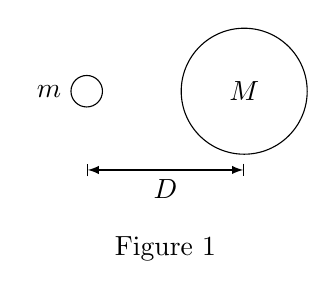
\begin{tikzpicture}
    \draw (0,0) circle (2mm) node[left=2mm] {$m$};
    \draw (2,0) circle (8mm) node {$M$};
    \draw[|<->|] (0,-1) -- ++(2,0) node[below,pos=0.5] {$D$};
    \node at (1,-2) {Figure 1};
\end{tikzpicture}
\hspace{1.5cm}
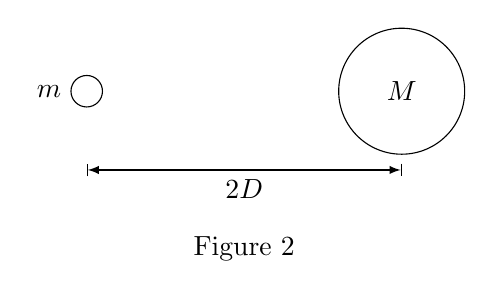
\begin{tikzpicture}
    \draw (0,0) circle (2mm) node[left=2mm] {$m$};
    \draw (4,0) circle (8mm) node {$M$};
    \draw[|<->|] (0,-1) -- ++(4,0) node[below,pos=0.5] {$2D$};
    \node at (2,-2) {Figure 2};
\end{tikzpicture}
\end{center}
\end{example}

\textit{Solution}:

In Figure 1, the gravitational force is

\begin{equation*}
    F = \frac{GmM}{D^2}
\end{equation*}

Let $F^\prime$ be the force in Figure 2, when the distance has doubled. Then,

\begin{equation*}
    F^\prime = \frac{G m M}{(2D)^2} = \frac{GmM}{4D^2}
\end{equation*}

To find the factor of change, we take the ratio $F^\prime/F$:

\begin{equation*}
    \frac{F^\prime}{F} = \frac{\left(\displaystyle \frac{GmM}{4D^2}\right)}{\left(\displaystyle \frac{GmM}{D^2}\right)} = \left(\frac{\cancel{GmM}}{4\cancel{D^2}}\right) \left(\frac{\cancel{D^2}}{\cancel{GmM}}\right) = \frac{1}{4}
\end{equation*}

which reduces to

\begin{equation*}
    \frac{F^\prime}{F} = \frac{1}{4}
\end{equation*}

Therefore,$F^\prime = \frac{F}{4}$. That is, the gravitational force in Figure 2 is $\frac{1}{4}$ of the force in Figure 1. \hfill $\blacksquare$

\subsubsection{Ranking the Gravitational Force at Various Distances}

\subsubsection{Ranking the Gravitational Force of Various Masses}

\subsubsection{The Gravitational Field}

In general, the strength of the gravitational field on the surface of a massive planetary body is given by

\begin{equation*}
    g = \frac{GM}{R^2}
\end{equation*}

where $G = \SI{6.67e-11}{N\cdot m^2/kg^2}$ is the gravitational constant, $M$ is the planet's mass, and $R$ is the planet's radius.

\begin{example}
    Find the \textit{exact} value, rounded to one decimal place, of the gravitational field strength on Earth. The mass and radius of Earth are $M = \SI{5.97e24}{kg}$ and $R = \SI[group-separator={,}]{6378000}{m}$. 
\end{example}

\textit{Solution:}

\begin{equation*}
    g = \frac{GM}{R^2} = \frac{(\SI{6.67e-11}{N\cdot m^2/kg^2})(\SI{5.97e24}{kg})}{(\SI{6.378e6}{m})^2} = \boxed{\SI{9.8}{N/kg}}
\end{equation*}

\hfill $\blacksquare$

\subsubsection{Calculating Force using the Law of Gravitation}

\subsubsection{The Gravitational Field Strength of Earth, g}


The gravitational field strength, $g$:

\begin{equation*}
    g = \SI{10}{N/kg} \qquad \text{(on Earth)}
\end{equation*}

\subsubsection{Mass and Weight}

\textbf{\Gls{mass}} is \glsdesc{mass}. It does not change based on location. In equations it is represented as $m$.

\textbf{\Gls{weight}} is \glsdesc{weight}. Being a force, weight is measured in newtons. It changes depending on location. In equations weight can be represented as $w$, $F_w$, or $F_g$.

\begin{center}
    \begin{tabular}{c|c}
        \textbf{Weight} & \textbf{Mass} \\ \hline
        force of gravity on an object & amount of matter \\ \hline
        measured in newtons (N) & measured in kilograms (kg) \\ \hline
        variable: $w$ & variable: $m$ \\ \hline
        vector (magnitude and direction) & scalar (magnitude only) \\ \hline
        e.g., $w = \SI{120}{N}$ down & e.g., $m = \SI{5}{kg}$ \\ \hline
        subject to change & does not change (constant) 
    \end{tabular}
\end{center}


Using a spring scale, you can plot the weight (force of gravity) as a function of mass, using a variety of masses, as shown below.

\begin{center}
\begin{minipage}[c][5cm][c]{0.3\textwidth}
\centering
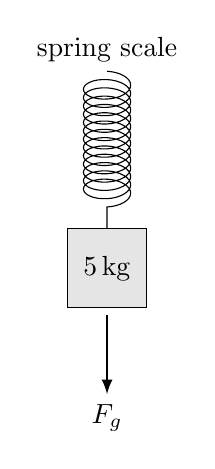
\begin{tikzpicture}
    \draw[decorate,decoration={coil,segment length=3pt,post length=2mm,pre length=0mm,amplitude=3mm}] (0,0) node[above] {spring scale} -- ++(0,-2);
    \begin{scope}[shift={(-0.5,-3)}]
        \draw[fill=black!10] (0,0) rectangle (1,1) node[pos=0.5] {\SI{5}{kg}};
        \draw [thick,->,yshift=-1mm] (0.5,0) -- ++(0,-1) node[below] {$F_g$};
    \end{scope}
\end{tikzpicture}
\end{minipage}%
\begin{minipage}[c][5cm][c]{0.45\textwidth}
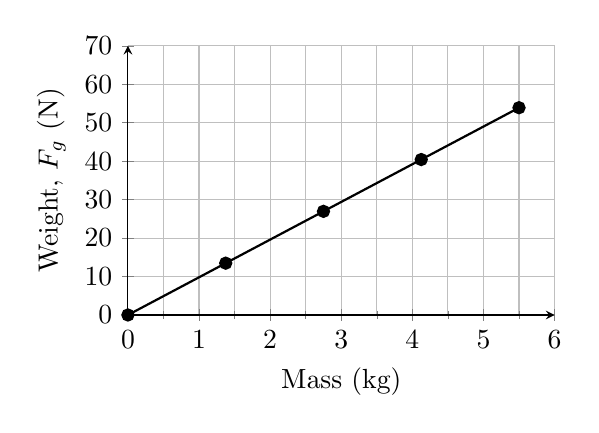
\begin{tikzpicture}
    \begin{axis}[height=5cm,width=7cm,
        axis lines=left,
        ylabel={Weight, $F_g$ (N)},
        xlabel={Mass (kg)},
        ymin=0,ymax=70,
        xmin=0,xmax=6,
        ytick={0,10,...,70},
        xtick={0,1,...,6},
        grid=both,
        minor x tick num=1,
    ]
        \addplot[thick,domain=0:5.5,mark=*,samples=5] {9.8*x};
    \end{axis}
\end{tikzpicture}
\end{minipage}
\end{center}

On Earth, the slope of this graph is about \SI{10}{N/kg}, because the gravitational field strength $g$ is \SI{10}{N/kg}.

\subsubsection{Calculating Force using Mass and Gravitational Field Strength}

Weight, or the force of gravity on an object of mass $m$, is calculated as

\begin{equation*}
    F_g = m g
\end{equation*}

In words,

\begin{equation*}
    \text{weight} = \text{mass} \times \SI{10}{N/kg}
\end{equation*}

\begin{example}
What is the weight of a 12\,kg box?
\end{example}

\textit{Solution:}

\begin{equation*}
    w = mg = (\SI{12}{kg})(\SI{10}{m/s^2}) = \boxed{\SI{120}{N}}    
\end{equation*}

\hfill $\blacksquare$

\subsection{Forces from Surfaces}

\subsubsection{Normal Force and Frictional Force}

A \textbf{\gls{contact force}} is \glsdesc{contact force}. Examples of contact forces include:

\begin{itemize}[topsep=0pt,itemsep=0pt]
    \item applied force ($F_\mathrm{A}$): e.g., kicking a ball
    \item tension force ($F_\mathrm{T}$): e.g., pulling a box with a rope
    \item spring force ($F_\mathrm{s}$): e.g., jumping on a pogo stick
\end{itemize}


Forces that come from a surface are called normal forces ($F_\mathrm{N}$). A \textbf{\gls{normal force}} is \glsdesc{normal force}. Normal forces are contact forces (due to objects touching a surface), are perpendicular to the surface, and are not always vertical.

\begin{center}
\begin{tikzpicture}
    \draw (0,0) -- (4,0);
    \draw[thick] (1.5,0) rectangle ++(1,1);
    \fill (2,0.5) circle (2pt);
    \draw[->] (2,0.5) -- ++(0,+1.3) node[above] {$F_\mathrm{N}$};
    \draw[->] (2,0.5) -- ++(0,-1.3) node[below] {$F_g$};
\end{tikzpicture}
\hspace{1.5cm}
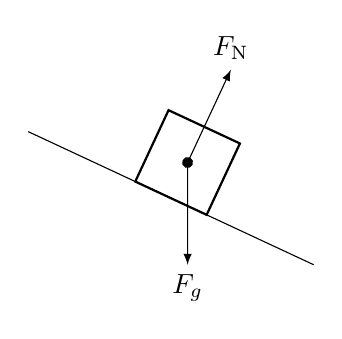
\begin{tikzpicture}[rotate=-25]
    \draw (0,0) -- (4,0);
    \draw[thick] (1.5,0) rectangle ++(1,1);
    \fill (2,0.5) circle (2pt);
    \draw[->] (2,0.5) -- ++(0,+1.3) node[above] {$F_\mathrm{N}$};
    \draw[->] (2,0.5) -- ++({1.3*sin(25)},{-1.3*cos(25)}) node[below] {$F_g$};
\end{tikzpicture}
\end{center}

The \textbf{\gls{frictional force}} ($F_f$) is \glsdesc{frictional force}. Friction is parallel to the surface.

\begin{center}
\begin{tikzpicture}
    \draw (0,0) -- (4,0);
    \draw[thick] (1.5,0) rectangle ++(1,1);
    \fill (2,0.5) circle (2pt);
    \draw[->] (2,0.5) -- ++(0,+1.3) node[above] {$F_\mathrm{N}$};
    \draw[->] (2,0.5) -- ++(0,-1.3) node[below] {$F_g$};
    \draw[->] (2,0.5) -- ++(+2,0) node[right] {$F_\mathrm{A}$};
    \draw[->] (2,0.5) -- ++(-2,0) node[left] {$F_f$};
\end{tikzpicture}
\end{center}

There are two types of friction. \textbf{Static friction} occurs between the surfaces of two objects that are not moving and will oppose the tendency of one object to move across the other. Static friction can change magnitude to prevent motion up to a maximum value. When this maximum value is overcome, the object starts moving. \textbf{Kinetic friction} occurs between the surfaces of two objects that \textit{are} moving relative to one another. Kinetic friction is a constant value.

\begin{center}
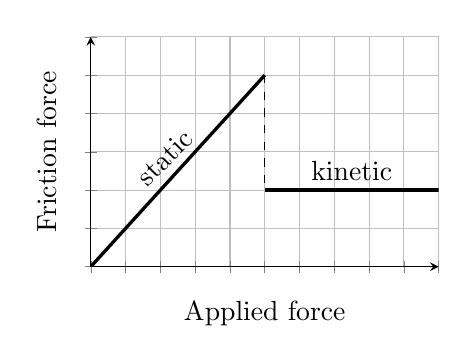
\begin{tikzpicture}
    \begin{axis}[height=4.5cm,width=6cm,
        axis lines=left,
        ylabel={Friction force},
        xlabel={Applied force},
        ymin=0,ymax=6,
        xmin=0,xmax=10,
        grid=both,
        ytick={0,1,...,6},
        xtick={0,1,...,10},
        yticklabels=\empty,
        xticklabels=\empty,
    ]
        \addplot[very thick] coordinates{(0,0)(5,5)};
        \addplot[dashed] coordinates{(5,5)(5,2)};
        \addplot[very thick] coordinates{(5,2)(10,2)};
        \node[rotate=45,above] at (2.5,2.5) {static};
        \node[above] at (7.5,2) {kinetic};
    \end{axis}
\end{tikzpicture}
\end{center}

The amount of friction acting on an object is determined by the roughness of the surface and how ``pushed together'' the object and surface are. Friction is related to the coefficient of friction ($\mu$).

\begin{itemize}[topsep=0pt,itemsep=0pt]
    \item The coefficient $\mu$ is greater for rougher surfaces
    \item The coefficient $\mu$ is zero for frictionless surfaces
\end{itemize}

Friction is also related to the normal force. If the normal force increases due to a change in the scenario, then friction will increase too. 

\subsubsection{Why the Normal and Gravitational Forces are not Force Pairs}

\begin{example}
A 3\,kg book rests on a table. Find the normal force.
\end{example}

\begin{center}
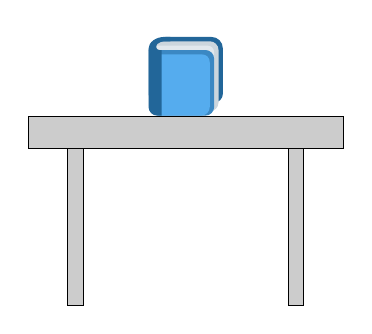
\begin{tikzpicture}
    \draw[fill=black!20] (0,0) rectangle ++(4,0.4);
    \draw[fill=black!20] (0.5,0) rectangle ++(0.2,-2);
    \draw[fill=black!20] (3.3,0) rectangle ++(0.2,-2);
    \node[above=2.9mm] at (2,0) {\twemoji[height=1cm]{blue book}};
\end{tikzpicture}
\end{center}

Recall: Normal force is the perpendicular force that an surface exerts to support the weight of an object. 

Normal force is equal in magnitude to weight, opposite in direction

Weight is

\begin{equation*}
    w = mg = (\SI{3}{kg})(\SI{10}{m/s^2}) = \SI{30}{N} \quad \text{down}
\end{equation*}

Magnitude of the normal force is

\begin{equation}
    F_\mathrm{n} = \left|w\right| = \SI{30}{N}
\end{equation}

and the direction is up.

\hfill $\blacksquare$

\subsubsection{How Motion, Surfaces, and the Normal Force affect the Frictional Force}

\subsection{Applied Forces}

\subsubsection{Tension Force}

\subsubsection{Identifying other Applied Forces}

\subsection{Analyzing Forces using Motion}

\subsubsection{Free Body Diagrams from Word Problems}

\subsubsection{Net Resultant Force using Vector Addition}

A \textbf{\gls{vector}} is \glsdesc{vector}. Vectors are represented by arrows. Consider vector $\vec{A}$ with a magnitude of 5 units at \ang{60} above the horizontal, shown below. The magnitude of this vector is

\begin{equation*}
    A = \left|\vec{A}\right| = 5\,\mathrm{units}
\end{equation*}

\begin{center}
\begin{minipage}{0.3\textwidth}
\centering

Vector $\vec{A}$:

\bigskip

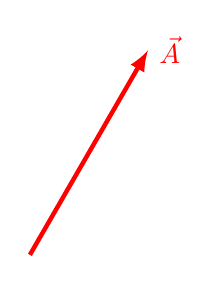
\begin{tikzpicture}[x=3cm,y=3cm]
    \draw[thick,->,ultra thick, red] (0,0) -- ({cos(60)},{sin(60)}) node[right] {$\vec{A}$};
\end{tikzpicture}
\end{minipage}%
\begin{minipage}{0.65\textwidth}
\centering

Vector $\vec{A}$ annotated with magnitude ($A$) and direction ($\theta$):

\bigskip

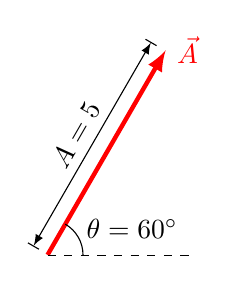
\begin{tikzpicture}[x=3cm,y=3cm]
    \draw[ultra thick,->,red] (0,0) -- ({cos(60)},{sin(60)}) node[right] {$\vec{A}$};
    \draw[|<->|,rotate=60,yshift=6pt,transform shape] (0,0) -- (1,0) node[above,pos=0.5] {$A = 5$};
    \draw (0.15,0) arc (0:60:0.15) node[right=2pt,pos=0.8] {$\theta = \ang{60}$};
    \draw[very thin,dashed] (0,0) -- (0.6,0);
\end{tikzpicture}
\end{minipage}
\end{center}

By placing the vector on the $xy$-coordinate plane, we can visualize and calculate the horizontal and vertical components vector $\vec{A}$. The horizontal component is called the $x$-component ($\vec{A}_x$), and the vertical is called the $y$-component ($\vec{A}_y$). Because the components $\vec{A}_x$ and $\vec{A}_y$ form a right triangle with vector $\vec{A}$, we can use trigonometry---specifically, the SOH\,CAH\,TOA method---to find magnitudes of the components. Also, we can relate the magnitudes of the components to the magnitude of the vector with the Pythagorean theorem. These relationships are summarized below.

\begin{center}
\begin{minipage}{0.3\textwidth}
\centering
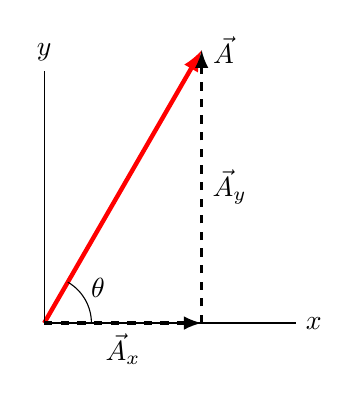
\begin{tikzpicture}[x=4cm,y=4cm]
    \draw[thick,->,ultra thick, red] (0,0) -- ({cos(60)},{sin(60)}) node[right,black] {$\vec{A}$};
    \draw (0,0) -- (0.8,0) node[right] {$x$};
    \draw (0,0) -- (0,0.8) node[above] {$y$};
    \draw[very thick,dashed,->] (0,0) -- ({cos(60)},0) node[below,pos=0.5] {$\vec{A}_x$};
    \draw[very thick,dashed,->] ({cos(60)},0) -- ++(0,{sin(60)}) node[right,pos=0.5] {$\vec{A}_y$};
    \draw (0.15,0) arc (0:60:0.15) node[right=2pt,pos=0.8] {$\theta$};
\end{tikzpicture}
\end{minipage}%
\begin{minipage}{0.3\textwidth}
\begin{gather*}
    A_x = A\cos{\theta} \\[2pt]
    A_y = A\sin{\theta} \\[2pt]
    A_x^2 + A_y^2 = A^2 \\[2pt]
    \tan{\theta} = \frac{A_y}{A_x}
\end{gather*}
\vspace{2em}
\end{minipage}
\end{center}

Notice that $\theta$ is measured as the angle between the vector and the adjacent $x$-axis. These relationships hold in any quadrant of the $xy$-plane, calculators will give negative values if the horizontal or vertical components point left or right, respectively, as shown below:

\begin{center}
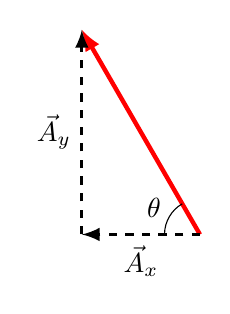
\begin{tikzpicture}[x=3cm,y=3cm]
    \draw[thick,->,ultra thick, red] (0,0) -- ({-cos(60)},{sin(60)});
    \draw[very thick,dashed,->] (0,0) -- ({-cos(60)},0) node[below,pos=0.5] {$\vec{A}_x$};
    \draw[very thick,dashed,->] ({-cos(60)},0) -- ++(0,{sin(60)}) node[left,pos=0.5] {$\vec{A}_y$};
    \draw (-0.15,0) arc (180:120:0.15) node[left=2pt,pos=0.8] {$\theta$};
\end{tikzpicture}   
\hspace{1.5cm}
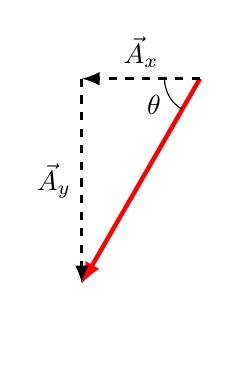
\begin{tikzpicture}[x=3cm,y=3cm]
    \draw[thick,->,ultra thick, red] (0,0) -- ({-cos(60)},{-sin(60)});
    \draw[very thick,dashed,->] (0,0) -- ({-cos(60)},0) node[above,pos=0.5] {$\vec{A}_x$};;
    \draw[very thick,dashed,->] ({-cos(60)},0) -- ++(0,{-sin(60)}) node[left,pos=0.5] {$\vec{A}_y$} node[below,white] {$\vec{A}_y$};
    \draw (-0.15,0) arc (180:240:0.15) node[left=2pt,pos=0.8] {$\theta$};
\end{tikzpicture}  
\hspace{1cm}
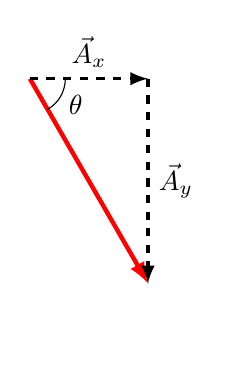
\begin{tikzpicture}[x=3cm,y=3cm]
    \draw[thick,->,ultra thick, red] (0,0) -- ({cos(60)},{-sin(60)});
    \draw[very thick,dashed,->] (0,0) -- ({cos(60)},0) node[above,pos=0.5] {$\vec{A}_x$};;
    \draw[very thick,dashed,->] ({cos(60)},0) -- ++(0,{-sin(60)}) node[right,pos=0.5] {$\vec{A}_y$} node[below,white] {$\vec{A}_y$};;
    \draw (0.15,0) arc (0:-60:0.15) node[right=2pt,pos=0.8] {$\theta$};
\end{tikzpicture}  
\end{center}

\begin{example}
Given vector $\vec{R}$ below, draw its horizontal and vertical components.

\begin{center}
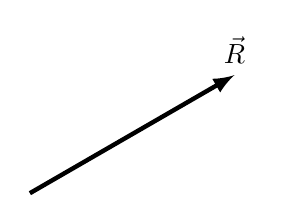
\begin{tikzpicture}[x=3cm,y=3cm]
    \draw[ultra thick,->] (0,0) -- ({cos(30)},{sin(30)}) node[above] {$\vec{R}$};
\end{tikzpicture}
\end{center}
\end{example}

\textit{Solution}:

Various examples of vector and their components are shown above, but it's often better to draw the components from the tail of the vector, like this:


\begin{center}
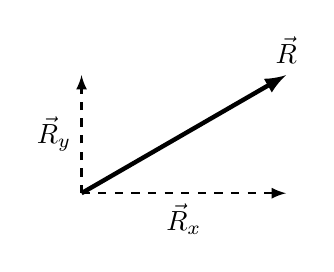
\begin{tikzpicture}[x=3cm,y=3cm]
    \draw[ultra thick,->] (0,0) -- ({cos(30)},{sin(30)}) node[above] {$\vec{R}$};
    \draw[thick,->,dashed] (0,0) -- ({cos(30)},0) node[below,pos=0.5] {$\vec{R}_x$};
    \draw[thick,->,dashed] (0,0) -- (0,{sin(30)}) node[left,pos=0.5] {$\vec{R}_y$};
\end{tikzpicture}
\end{center}

\hfill $\blacksquare$

\subsubsection{Solving for Unknown Force, Mass, or Acceleration}

\subsubsection{Solving for Other Unknowns}



\fi

\clearpage


\section{One-Dimensional Motion}

\ifShowUnitVI

\subsection{Free Fall Concepts}

\subsubsection{Gravitational Field Strength and Acceleration due to Gravity on Earth}

% \textit{Learning expectation}: \glsdesc{OSLE 6.1.a}

\textbf{\Gls{free fall}} is \glsdesc{free fall}.

\subsubsection{Why Objects near Earth's Surface Fall at the
Same Rate}


% \textit{Learning expectation}: \glsdesc{OSLE 6.1.b}

\subsubsection{Final Velocity and Time in Free Fall}


% \textit{Learning expectation}: \glsdesc{OSLE 6.1.c}

\subsubsection{Motion of Objects Dropped or Thrown using Multiple Representations}


% \textit{Learning expectation}: \glsdesc{OSLE 6.1.d}

\subsubsection{Gravitational Force, Impulse, and Work Done by Earth}


% \textit{Learning expectation}: \glsdesc{OSLE 6.1.e}

\subsection{Solving Constant Acceleration Problems}

\subsubsection{Describing What is Known About Motion}

The \textbf{\gls{kinematic equations}} are \glsdesc{kinematic equations}. They are

\begin{align}
    v_f &= v_i + at \\[1ex]
    \Delta x &= v_i t + \frac{1}{2}at^2 \\[1ex]
    v_f^2 &= v_i^2 + 2 a \Delta x \\[1ex]
    \Delta x &= \frac{1}{2} \left(v_i + v_f\right) t
\end{align}

where $v_f$ is final velocity, $v_i$ is initial velocity, $a$ is acceleration, $t$ is time, and $\Delta x$ is displacement. 

The kinematic equations for one-dimensional free fall motion are

\begin{align}
    v_f &= v_i - gt \label{xgXRE} \\[1ex]
    \Delta y &= v_i t - \frac{1}{2}gt^2 \\[1ex]
    v_f^2 &= v_i^2 - 2g\Delta y \\[1ex]
    \Delta y &= \frac{1}{2}\left(v_i + v_f\right) t
\end{align}

where $g = \SI{10}{m/s^2}$ is the strength of the gravitational field near the surface of the Earth, also known as the acceleration due to gravity.

\subsubsection{Solving for Unknown Quantities: Horizontal Motion}

\subsubsection{Solving for Unknown Quantities: Vertical Motion}

\begin{example}
    The JP Morgan Chase Tower is the tallest building in Houston. If you drop a bowling ball from rest from the top of the building, it takes 7.81 seconds for it to strike the ground below. How tall is the building?
\end{example}

\textit{Solution}:

We know time is $t = \SI{7.81}{s}$ and the magnitude of gravitational acceleration is $g = \SI{10}{m/s^2}$. Since the object is dropped from rest, initial velocity is $v_i = 0$. The ball's vertical displacement is

\begin{align*}
    \Delta y &= v_i t - \frac{1}{2}g t^2 \\[1ex]
    &= (\SI{0}{m/s})(\SI{7.81}{s}) - \frac{1}{2} (\SI{10}{m/s^2})(\SI{7.81}{s})^2 \\[1ex]
    &= -\SI{305}{m}
\end{align*}

This vertical displacement must be equal in magnitude to the height of the building. Therefore, the building's height is \SI{305}{m}.

\hfill $\blacksquare$

\begin{example}
The Burj Kalifa, the tallest building in the world, is 830 meters tall. How long would it take a bowling ball that is released from rest from the top of the building to strike the ground?
\end{example}

\textit{Solution}:

The displacement of the ball has the same magnitude as the height of the building, but it's negative since the ball moves downward:

\begin{equation*}
    \Delta y = -\SI{830}{m}
\end{equation*}

We are given that the ball is dropped from rest, so the initial velocity is $v_i = \SI{0}{m/s}$. And gravitational acceleration has a magnitude of $g = \SI{10}{m/s^2}$. These quantities are related by the kinematic equation

\begin{equation*}
    \Delta y = v_i t - \frac{1}{2}gt^2
\end{equation*}

Plugging in numbers leads to

\begin{align*}
    -\SI{830}{m} &= (\SI{0}{m/s}) t - \frac{1}{2}\left(\SI{10}{m/s^2}\right) t^2 \\[1ex]
    &= -\left(\SI{5}{m/s^2}\right) t^2
\end{align*}

To solve for time, we divide both sides by 5 and take the square root:

\begin{equation*}
    t = \sqrt{\frac{\SI{830}{m}}{\SI{5}{m/s^2}}} = \boxed{\SI{12.9}{s}}
\end{equation*}

Therefore, it take 12.9 seconds for the ball to strike the ground.

\hfill $\blacksquare$


\subsubsection{Multi-Step Problems with Kinematic Equations}

\fi

\clearpage

\section{Motion in Two Dimensions}

\ifShowUnitVII

\subsection{Factors That Affect Projectile Trajectory}
\subsubsection{Trajectory, Hang Time, Max Height, and Range}
\subsubsection{How Initial Velocity, Launch Height, Launch Angle, and Mass Affect Motion}


\Glsdesc{projectile} is called a \textbf{\gls{projectile}}. Thus, \textbf{\gls{projectile motion}} is \glsdesc{projectile motion}. The \textbf{\gls{trajectory}} is \glsdesc{trajectory}. The shape of a trajectory is a parabola, shown below:

\begin{center}
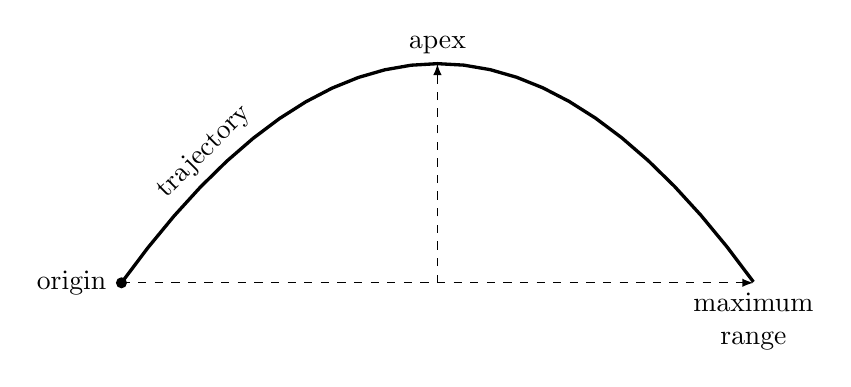
\begin{tikzpicture}
    \begin{axis}[height=4.5cm,width=10cm,
        axis lines=none,
        ymin=0,ymax=13,
        xmin=0,xmax=30,
        clip=false,
    ]
    \addplot[domain=0:28.6,very thick] {trajectoryequation(x,18,60)} node[rotate=45,pos=0.2,above] {trajectory};
    \draw[->,dashed] (0,0) -- (28.6,0) node[below,align=center] {maximum\\range};
    \draw[->,dashed] (14.3,0) -- ++(0,12.38) node[above] {apex};
    \fill (0,0) circle (2pt) node[left=2pt] {origin};
    \end{axis}
\end{tikzpicture}
\end{center}

There's a special name for the point at which a projectile reaches peak vertical position: The \textbf{\gls{apex}} is \glsdesc{apex}.



A projectile may be launched at different velocities, from different heights, and at different angles, and these changes could produce changes in the trajectory.

\begin{center}
\begin{tikzpicture}[declare function={t(\x)=\x/(18*cos(45));}]
    \begin{axis}[width=16cm,,height=10cm,
        axis lines=none,
        ylabel={$y$ (m)},
        xlabel={$x$ (m)},
        ymin=0,ymax=20,
        xmin=0,xmax=45,
        ytick={0,2,...,20},
        xtick={0,5,...,45},
        minor x tick num=1,
        grid=both,
        clip=false,
    ]
    \addplot[domain=0:40,red,thick] {trajectoryequation(x,18,45)+10};
    \def\myscale{0.3}
    \pgfplotsinvokeforeach{0,5,10,21,26,31,36,40}{
            \draw[fill=black] (#1,{trajectoryequation(#1,18,45)+10}) circle (2pt);
            \draw[dashed,->] (#1,{trajectoryequation(#1,18,45)+10}) -- ++(0,{\myscale*(18*sin(45) - 9.8*t(#1))});
            \draw[dashed,->] (#1,{trajectoryequation(#1,18,45)+10}) -- ++({\myscale*18*cos(45)},0);
            \draw[thick,->] (#1,{trajectoryequation(#1,18,45)+10}) -- ++({\myscale*18*cos(45)},{0.3*(18*sin(45) - 9.8*t(#1))});
            }
            
    %...For the apex:
    \draw[fill=black] (16.51,{trajectoryequation(16.51,18,45)+10}) circle (2pt);
    \draw[thick,->] (16.51,{trajectoryequation(16.51,18,45)+10}) -- ++({\myscale*18*cos(45)},0);

    %...For the initial point:
    \draw (0,{trajectoryequation(0,18,45)+10}) ++ (0,{\myscale*(18*sin(45))}) node[above] {$v_{iy}$};
    \draw (0,{trajectoryequation(0,18,45)+10}) ++ ({\myscale*(18*cos(45))},0) node[right] {$v_{ix}$};
    \draw (0,{trajectoryequation(0,18,45)+10}) ++ ({\myscale*(18*cos(45))},{\myscale*(18*sin(45))}) node[above left] {$v_i$};
    \end{axis}
\end{tikzpicture}
\end{center}


A projectile has horizontal and vertical motions. These are independent, meaning they don't influence one another. Vertical and horizontal motions are analyzed them separately, along perpendicular axes.

\subsection{Horizontally Launched Projectiles}
\subsubsection{Describing Vertical and Horizontal Motion Using Multiple Representations}

\subsubsection{Horizontal and Vertical Components with Vector Addition}

\subsubsection{Word Problems About Horizontally Launched Projectiles}

A \textbf{\gls{horizontally launched projectile}} is, as the name suggests, \glsdesc{horizontally launched projectile}. The figure below is a motion map showing similarities and differences between a dropped object and a horizontally launched one.

\begin{center}
\begin{tikzpicture}[x=4mm,y=4mm]
    \draw[step=1,lightgray,thin] (0,0) grid (24,15);
    \pgfplotsinvokeforeach{0,0.35,0.70,1.05,1.4,1.75}{
        \draw[red,dashed,thick] (1,{15-0.5*9.8*(#1)^2}) -- ++({10*#1 +4},0);
        \fill (1,{15-0.5*9.8*(#1)^2}) circle (3pt);
    }
    \pgfplotsinvokeforeach{0,0.35,0.70,1.05,1.4,1.75}{
        \fill ({10*#1+5},{15-0.5*9.8*(#1)^2}) circle (3pt);
    }
    \draw[<-,thick,xshift=-3pt,yshift=3pt] (1,15) -- ++(-1.5,1.5) node[above] {dropped};
    \draw[<-,thick,xshift=+3pt,yshift=3pt] (5,15) -- ++(+1.5,1.5) node[above] {horizontally launched};
\end{tikzpicture}
\end{center}

The red dashed lines indicate that the object dropped into free fall is falling at the \textit{same rate} as the horizontally launched projectile. Therefore, we should separate projectile motion into two components, one along horizontal axis and the other along the vertical axis. The following worked examples show how to do~this.

\begin{example} \label{ER19WG}
    A cannonball is launched horizontally from the Statue of Liberty's \href{https://www.nps.gov/stli/planyourvisit/images/Statue-from-Fort-Wood-up-3_1.jpg?maxwidth=1300&maxheight=1300&autorotate=false}{base pedestal}, which is \SI{45}{m} above ground, at a speed of \SI{16}{m/s}. How much time will it take the projectile to strike the ground?

\begin{center}
    \begin{tikzpicture}
        \begin{axis}[width=6cm,height=6cm,
            ticks=none,
            xmin=0,xmax=50,
            ymin=0,ymax=50,
            clip=false,
            axis lines*=left,
        ]
            \draw[thick,->] (0,45) -- ++(2cm,0) node[right] {\SI{16}{m/s}};
            \addplot[domain=0:48,thick,dashed] {trajectoryequation10(x,16,0)+45};
            \fill (0,45) circle (3pt);
            \draw[<->,thin,xshift=-5pt] (0,0) -- ++(0,45) node[left,pos=0.5] {\SI{45}{m}};
        \end{axis}
    \end{tikzpicture}
\end{center}
\end{example}

\textit{Solution:}

From the pedestal to the ground, the projectile's displacement is $\Delta y = \SI{-45}{m}$ and during the fall its motion was governed by the kinematic equation

\begin{equation*}
    \Delta y = v_{iy} t - \frac{1}{2} g t^2
\end{equation*}

For a horizontally, the $y$-component of the initial velocity is zero: $v_{iy} = 0$. So, the equation reduces to

\begin{equation*}
    \Delta y = -\frac{1}{2}gt^2
\end{equation*}

Solving for time leads to

\begin{align*}
    t &= \sqrt{-\frac{2\Delta y}{g}} \\[1ex]
    &= \sqrt{-\frac{2(-\SI{45}{m})}{\SI{10}{m/s^2}}} \\[1ex]
    &= \boxed{\SI{3.0}{s}}
\end{align*}

\hfill $\blacksquare$

\begin{example} \label{ADuHT8}
    How does the answer to Example \ref{ER19WG}, $t=\SI{3}{s}$, change if the projectile's initial speed is doubled?
\end{example}

\textit{Solution:}

The time doesn't change, since both projectiles fall from the same height at the same rate.

\hfill $\blacksquare$

\begin{example} \label{mT7mjd}
    When a ball is horizontally launched from a height $h$, it takes the ball \SI{4.0}{s} to strike the ground. How long will take the same ball to strike ground if it is horizontally launched from a height $4h$?
\end{example}

\textit{Solution:}

In Example \ref{ER19WG} we saw that the kinematic equation may be solved for time as

\begin{equation*}
    t = \sqrt{-\frac{2\Delta y}{g}}
\end{equation*}

This equation shows that time is proportional to the square root of displacement:

\begin{equation*}
    t \propto \sqrt{\left|\Delta y\right|}
\end{equation*}

So, increasing the height by a factor of 4 increases the time by a factor of $\sqrt{4}$, or 2. Therefore the new elapsed time is \SI{8.0}{s}.

\hfill $\blacksquare$

\textbf{\Gls{impact speed}} is \glsdesc{impact speed}. The impact velocity is the vector representing the impact speed and its direction. 

\begin{center}
    \begin{tikzpicture}
        \begin{axis}[width=5cm,height=4.5cm,
            ticks=none,
            ymin=0,ymax=11,
            xmin=0,xmax=15,
            clip=false,
            axis lines*=left,
        ]
        \addplot[domain=0:14.98,thick,dashed] {trajectoryequation10(x,10,0)+11};
        \fill (14.98,0) circle (2pt);
        \draw[->,ultra thick] (14.98,0) -- ++({6*cos(56)},{-6*sin(56)}) node[above right] {impact velocity};
        \end{axis}
    \end{tikzpicture}
\end{center}



The impact speed $v$ is the magnitude of the vector addition of the horizontal and vertical components of velocity at impact.


\begin{center}
\begin{tikzpicture}[x=3cm,y=3cm]
    \draw[->,thick] (0,0) -- ({cos(56)},{-sin(56)}) node[left=2pt,pos=0.5] {$v$};
    \draw[->,thick,xshift=1mm] (0,0) -- ({cos(56)},0) node[above,pos=0.5] {$v_x$};
    \draw[->,thick,xshift=1mm] ({cos(56)},0) -- ({cos(56)},{-sin(56)}) node[right,pos=0.5] {$v_y$};
\end{tikzpicture}
\end{center}

Thus, it is calculated by the Pythagorean theorem as

\begin{equation} \label{KBgFF}
    v = \sqrt{v_x^2 + v_y^2}
\end{equation}

where $v_x$ and $v_y$ are the horizontal and vertical components of velocity at the moment of impact.

\begin{example}
    In Example \ref{ER19WG}, a cannonball was launched near the State of Liberty from a height of \SI{45}{m} at \SI{16}{m/s}. Find the speed of the projectile the instant it strikes the ground. (Find the impact speed.)
\end{example}

\textit{Solution}:

Impact speed is given by Equation \eqref{KBgFF}:

\begin{equation*}
    v = \sqrt{v_x^2 + v_y^2}
\end{equation*}

The horizontal component of speed is the same as the initial speed, since horizontal acceleration is zero in projectile motion:

\begin{equation*}
    v_x = v_i = \SI{16}{m/s}
\end{equation*}

The vertical component of impact velocity is given by kinematic equation \eqref{xgXRE} with an initial vertical speed zero and an elapsed time of 3 seconds that was calculated in Example \ref{ER19WG}:

\begin{align*}
    v_y &= v_i - gt \\[1ex]
    &= \SI{0}{m/s} - (\SI{10}{m/s^2})(\SI{3.0}{s}) \\[1ex]
    &= -\SI{30}{m/s}
\end{align*}

The negative indicates the direction of the $y$-component of velocity is downward. Therefore,

\begin{align*}
    v &= \sqrt{v_x^2 + v_y^2} \\[1ex]
    &= \sqrt{(\SI{16}{m/s})^2 + (-\SI{30}{m/s})^2} \\[1ex]
    &= \boxed{\SI{34}{m/s}}
\end{align*}

\hfill $\blacksquare$

\clearpage

\subsection{Circular Motion}

\subsubsection{Uniform Circular Motion Using Multiple Representations}

\subsubsection{Quantities of Circular Motion}

\begin{example}
A car moves at a constant linear speed of \SI{24}{m/s} in a circular road of radius \SI{18}{m}. Calculate the car's centripetal acceleration.
\end{example}

\textit{Solution}:

We are given linear speed $v = \SI{24}{m/s}$ and radius of curvature $r = \SI{18}{m}$. The centripetal acceleration is

\begin{equation*}
    a_c = \frac{v^2}{r} = \frac{\left(\SI{24}{m/s}\right)^2}{\SI{18}{m}} = \boxed{\SI{32}{m/s^2}}
\end{equation*}

This acceleration points towards the center of the circle.

\hfill $\blacksquare$

\begin{example}
An object moves with constant speed $v_0$ in a circle of radius $r_0$ and experiences a centripetal acceleration $a_0$. 

\begin{center}
\begin{tikzpicture}[x=2cm,y=2cm]
    \draw[densely dashed] (0,0) circle (1);
    \draw (0,0) -- (1,0) node[below,pos=0.5] {$r_0$};
    \fill (0,0) circle (1pt);
    \draw[thick,->] ({cos(45)},{sin(45)}) -- ++({-cos(45)},{sin(45)}) node[pos=1.1] {$v_0$};
    \draw[thick,->] ({cos(45)},{sin(45)}) -- ++({-0.7*cos(45)},{-0.7*sin(45)}) node[pos=0.8,left=3pt] {$a_0$};
    \fill ({cos(45)},{sin(45)}) circle (3pt);
\end{tikzpicture}
\end{center}

If the object's speed changes to $\frac{1}{2}v_0$ and the radius stays constant, what is the new centripetal acceleration?
\end{example}

\textit{Solution}:

Let $a$ be the new centripetal acceleration, $v = \frac{1}{2}v_0$ be the new speed, and $r = r_0$ be the constant radius. The original acceleration is

\begin{equation*}
    a_0 = \frac{v_0^2}{r_0}
\end{equation*}


The new centripetal acceleration is

\begin{equation*}
    a = \frac{v^2}{r} = \frac{\left(\frac{1}{2}v_0\right)^2}{r_0} = \frac{\left(\frac{1}{2}\right)^2v_0^2}{r_0} = \frac{1}{4} \left(\frac{v_0^2}{r_0}\right) = \frac{1}{4} a_0
\end{equation*}

Therefore, when the speed is halved, the acceleration decreases to $\frac{1}{4}$ of the original acceleration.

\hfill $\blacksquare$



\subsection{Circular Motion and Orbiting Bodies}

\subsubsection{How Radius and Mass Affects Orbiting Systems}

\fi

\clearpage

\section{Conservation in Mechanical Systems}

\ifShowUnitVIII

\subsection{Physical Systems}

\subsubsection{Choices for a System}

A \textbf{\gls{system}} is \glsdesc{system}.

\subsubsection{Energy Stored in the Arrangement of Particles}
\subsubsection{Gravitational and Elastic Potential Energy}

\textbf{\Gls{gravitational potential energy}} ($E_g$) is \glsdesc{gravitational potential energy}.

The gravitational potential energy between two objects of mass $m_1$ and $m_2$ whose centers of mass are separated by distance $r$ is

\begin{equation*}
    E_g = -\frac{G m_1 m_2}{r}
\end{equation*}

When an object is raised from the surface of the Earth to a height $h$, there is an gain in gravitational potential energy of magnitude

\begin{equation*}
    \Delta E_g = mgh
\end{equation*}

\begin{center}
\begin{tikzpicture}
    \begin{scope}
        \clip (-3,0) -- (3,0) arc (0:180:3);
        \draw (0,0) node[opacity=0.3] {\twemoji[width=6cm]{globe showing Americas}};
    \end{scope}
    \draw (3,0) arc (0:180:3);
    \draw[densely dashed] (-2,3) node[left,align=center] {\small reference\\height} -- (2,3);
    \draw[<->] (0,0) -- (0,3) node[right,pos=0.5] {$R$};
    % \draw[<->] (0,3) -- (0,4) node[right,pos=0.5] {$y_0$};
    \draw[->] (0,3) -- (0,4) node[right,pos=0.5] {$h$};
    \fill[yshift=3pt] (0,4) circle (3pt) node[above=3pt] {$m$};
\end{tikzpicture}
\end{center}

In general, the reference height $y_0$ doesn't need to be at the surface (where $y_0 = 0$). It can be set at the top of a 6-meter ramp ($y_0 = \SI{6}{m}$) or on top of a tall building ($y_0 = \SI{100}{m}$). Furthermore, a vertical displacement $\Delta y$ above or below the reference height yields an increase or a decrease in gravitational potential energy, respectively. 

\begin{center}
\begin{tikzpicture}
    \begin{scope}
        \clip (-3,0) -- (3,0) arc (0:180:3);
        \draw (0,0) node[opacity=0.3] {\twemoji[width=6cm]{globe showing Americas}};
    \end{scope}
    \draw (3,0) arc (0:180:3);
    \draw[densely dashed] (-2,4) node[left,align=center] {\small reference\\height} -- (2,4);
    \draw[<->] (0,0) -- (0,3) node[right,pos=0.5] {$R$};
    \draw[<->] (0,3) -- (0,4) node[right,pos=0.5] {$y_0$};
    \draw[->] (0,4) -- (0,5) node[right,pos=0.5] {$\Delta y$};
    \fill[yshift=3pt] (0,5) circle (3pt) node[above=3pt] {$m$};
    \node[above=3pt,align=center] at (current bounding box.north) {\textit{Increase} in\\gravitational potential energy};
\end{tikzpicture}
\hspace{1cm}
\begin{tikzpicture}
    \begin{scope}
        \clip (-3,0) -- (3,0) arc (0:180:3);
        \draw (0,0) node[opacity=0.3] {\twemoji[width=6cm]{globe showing Americas}};
    \end{scope}
    \draw (3,0) arc (0:180:3);
    \draw[densely dashed] (-2,5) -- (2,5) node[right,align=center] {reference\\height};
    \draw[<->] (0,0) -- (0,3) node[right,pos=0.5] {$R$};
    \draw[|<->|] (-0.5,3) -- ++(0,2) node[left,pos=0.5] {$y_0$};
    \draw[->] (0,5) -- ++(0,-1.0) node[right,pos=0.5] {$\Delta y$};
    \fill[yshift=-3pt] (0,4) circle (3pt) node[right=3pt] {$m$};
    \node[above=3pt,align=center] at (current bounding box.north) {\textit{Decrease} in\\gravitational potential energy};
\end{tikzpicture}

\underline{Note:} Lengths in figures are not to scale.
\end{center}

Therefore, the general formula for the change in gravitational potential energy is

\begin{equation}
    \Delta E_g = mg \Delta y
\end{equation}

\begin{example} \label{J1Qehp}
A 2.0-kg ball gets kicked in the air to a maximum height of 15 meters. At the peak height, what is the change in gravitational potential energy of the ball-Earth system relative to the ground?
\end{example} 

\textit{Solution:} 

We are given mass and height: $m = \SI{2.0}{kg}$, $h = \SI{15}{m}$, and gravity is $\SI{10}{m/s^2}$. The unknown we are finding in gravitational potential energy: $\mathrm{PE_g} =\ ?$ By Eq.~(\ref{RlpJa5}),

\begin{equation*}
    \Delta E_g = mg \Delta y = (\SI{2.0}{kg})(\SI{10}{m/s^2})(\SI{15}{m}) =  \boxed{\SI{300}{J}}
\end{equation*}

\hfill $\blacksquare$

\subsubsection{Comparing Potential Energy}
\subsubsection{Multiple Representations for Total Mechanical Energy}
\subsubsection{Effects of Changing Physical Quantities on Energy}
\subsubsection{Calculations of Total Mechanical Energy}






% \textit{YouTube}: ``Chris Farley -- Greatest Entrance Ever'' by MyTalkShowHeroes (\href{https://youtu.be/_z9kdqDwA80}{link}). Watch the first 1:00 min. What does Chris Farley have a lot of? Energy. More specifically, kinetic energy.

\clearpage
% Kinetic energy moved to unit 1!!!

%\subsection{Conservation of Mechanical Energy} \label{KRxiCV}

\textbf{mechanical energy} is the sum of kinetic energy and potential energy. The law of conservation of mechanical energy says that for a closed system energy is conserved. This law is expressed as

\begin{equation} \label{QyLUh5}
    \mathrm{ME} = \mathrm{KE} + \mathrm{PE} = \mathrm{constant}
\end{equation}

but is more usefully written as

\begin{equation} \label{yOUj22}
    \mathrm{KE_i} + \mathrm{PE_i} = \mathrm{KE_f} + \mathrm{PE_f}
\end{equation}

If we replace each $\mathrm{KE}$ and $\mathrm{PE}$ with $\frac{1}{2}mv^2$ and $mgh$, respectively, the law of conservation of energy becomes

\begin{equation} \label{ZSmSin}
    \frac{1}{2} m v_i^2 + mgh_i  = 
    \frac{1}{2} m v_f^2 + mgh_f 
\end{equation}

\begin{example} \label{mUfgIz}
Tony Hawk starts from rest from the top of a 6-meter tall ramp. His mass is \SI{77}{kg}. What will be his kinetic energy at the bottom of the ramp? Assume no energy is lost to friction.


\begin{center}
\begin{tikzpicture}
\begin{axis}[width=8cm,height=3.5cm,
    clip=false,
    xmin=-5,xmax=5,ymin=0,ymax=6,
    axis lines=center,
    axis line style={draw=none},
    ticks=none,
]
\addplot[ultra thick,samples=100,
    domain=-2.5:2.5
]{x^2}; 
\node[below] at (0,0) {\texttt{bottom}};
\node[above] at (-2.5,6) {\texttt{top}};
\node[rotate=-45] at (-1.9,5.8) {\Strichmaxerl[2.5]};
\end{axis}
\end{tikzpicture}
\end{center}
\end{example} 

\textit{Solution:} 

By the law of conservation of mechanical energy (Eq.~\ref{yOUj22}), Hawk's mechanical energy is governed by the equation

\begin{equation*} 
    \mathrm{KE_i} + \mathrm{PE_i} = \mathrm{KE_f} + \mathrm{PE_f}
\end{equation*}

At the top, Hawk has no motion, so his initial kinetic energy is zero: $\mathrm{KE_i} = 0$. At the bottom, he loses all height above the ramp, so his gravitational potential energy is zero: $\mathrm{PE_f} = 0$. Therefore, conservation of energy reduces from

\begin{equation*}
    \cancel{\mathrm{KE_i}} + \mathrm{PE_i} = \mathrm{KE_f} + \cancel{\mathrm{PE_f}}
\end{equation*}

to

\begin{equation} \label{eosZpi}
    \mathrm{PE_i} = \mathrm{KE_f}
\end{equation}

This result means that all of Hawk's potential (stored) energy at the top of the ramp will be converted to kinetic (motion) energy when he reaches the bottom.

We are given Hawk's mass and his initial height above the ramp: $m = \SI{77}{kg}$ and $h_i = \SI{6}{m}$. The unknown we're looking for is his final kinetic energy, at the bottom of the ramp: $\mathrm{KE_f} =\ ?$ The given quantities are related by Eq.~(\ref{RlpJa5}), which provides Hawk's initial gravitational potential energy:

\begin{equation*}
    \mathrm{PE_i} = mgh_i = (77)(9.8)(6) = \SI{4527.6}{J} 
\end{equation*}

This energy, by Eq.~(\ref{eosZpi}), gets converted to Hawk's kinetic energy, so

\begin{equation*}
    \mathrm{KE_f} = \SI{4527.6}{J} 
\end{equation*}

This example is to show that all of Tony Hawk's gravitational potential energy at the top of the ramp was entirely converted to his kinetic energy at the bottom.

\hfill $\blacksquare$


\begin{example} \label{nQVUKM}
When Tony Hawk reaches the bottom, in Example \ref{mUfgIz}, what is his speed?
\end{example} 

\textit{Solution:} 

At the end of Example \ref{mUfgIz} we concluded that his kinetic energy at the bottom is 

\begin{equation*}
    \mathrm{KE_f} = \SI{4527.6}{J}
\end{equation*}

But his kinetic energy is

\begin{equation*}
    \mathrm{KE} = \frac{1}{2} m v^2
\end{equation*}

Substituting the given values leads to 

\begin{equation*}
    4527.6 = \frac{1}{2} \cdot 77 \cdot v^2
\end{equation*}

If we solve this equation for speed ($v$) then his speed is

\begin{equation*}
    v = \SI{10.8}{m/s}
\end{equation*}

\hfill $\blacksquare$

\subsection{Energy is Conserved}

\subsubsection{Energy of a System Before and After an Event}

\subsubsection{Law of Conservation of Energy}

\subsubsection{Power (Revisited)}


\subsection{Momentum is Conserved}

\subsubsection{Momentum, Force, and Impulse in Collisions and Explosions}

\subsubsection{Total Momentum Before and After Collisions and Explosions}

\subsubsection{Law of Conservation of Momentum}

\subsubsection{Solving for Unknown Quantities using Conservation of Momentum}



\begin{example}\label{EvkSMv}
A 0.057-kg tennis ball moves at $-\SI{12}{m/s}$ when it gets struck to a new velocity of $+\SI{48}{m/s}$. What is the ball's change in momentum?

\begin{center}
\begin{tikzpicture}
\begin{axis}[
    width=8cm,height=3cm,
    axis line style={draw=none},
    ticks=none,
    axis lines=left,
    xmin=0,xmax=10,
    ymin=0,ymax=10,
    clip=false
]
    \fill[black!10] (5.4,5) circle (2mm);
    \fill[black!20] (5.2,5) circle (2mm) node[black,above=8pt] {$-\SI{12}{m/s}$};
    \fill (5,5) circle (2mm);
\end{axis}
\end{tikzpicture}%
\begin{tikzpicture}
\begin{axis}[
    width=8cm,height=3cm,
    axis line style={draw=none},
    ticks=none,
    axis lines=left,
    xmin=0,xmax=10,
    ymin=0,ymax=10,
    clip=false
]
    \fill[black!10] (5,5) circle (2mm);
    \fill[black!20] (5.4,5) circle (2mm) node[black,above=8pt] {$+\SI{48}{m/s}$};
    \fill (5.8,5) circle (2mm);
\end{axis}
\end{tikzpicture}%
\end{center}
\end{example}

\textit{Solution}: 

We know the tennis ball's mass, initial velocity, and final velocity: $m = \SI{0.057}{kg}$, $v_i = -\SI{12}{m/s}$, and $v_f = +\SI{48}{m/s}$. We want to find change in momentum: $\Delta p =\ ?$ Change in momentum is

\begin{equation*}
    \Delta p  = m \left(v_f - v_i\right) = 0.057 \left(48 - \left(-12\right) \right) = 0.057 \left(48 + 12 \right) = \SI{3.42}{kg\,m/s}
\end{equation*}

\hfill $\blacksquare$

\begin{example}
During the 2007 French Open, \href{https://youtu.be/6b1NSgQZvdo}{Venus Williams} hit the fastest recorded serve in a premier women's match. The ball started at rest and reached a speed of \SI{58}{m/s} (\SI{130}{mph}). What was the average force exerted on the 0.057-kg tennis ball by Williams' racquet? Assume that the ball remained in contact with the racquet for \SI{5}{ms} (milliseconds) and accelerated horizontally.
\end{example}

\textit{Solution:} 

We are given final velocity, initial velocity, mass, and elapsed time: $v_f = \SI{58}{m/s}$, $v_i = \SI{0}{m/s}$, $m = \SI{0.057}{kg}$, and $\Delta t = \SI{5}{ms} = \SI{0.005}{s}$. (Note: $\SI{1}{ms} = \SI{1}{millisecond} = \SI{0.001}{s} = \SI{1e-3}{s}$.) We want to find the average net force: $F_{\text{net}} =\ ?$ Equation~(\ref{e8sC6q}) relates change in momentum to change in time as

\begin{equation*}
    F_{\text{net}} = \frac{\Delta p}{\Delta t}
\end{equation*}

The tennis ball's change in momentum is

\begin{equation*}
    \Delta p = m(v_f - v_i) = 0.057(58 - 0) = \SI{3.306}{kg\,m/s}
\end{equation*}

Therefore, the net force supplied by the racquet is

\begin{equation*}
    F_{\text{net}} = \frac{\Delta p}{\Delta t} = \frac{3.306}{0.005} = \SI{661}{N}
\end{equation*}
\vspace{0.1ex}

A force of \SI{661}{N} is about the weight of a 150-pound person!

\hfill $\blacksquare$

\begin{example} \label{W5BnBq} %%% Refer to this example at the beginning of the unit to motivate a better understanding of momentum. Our object is to scaffold up 
Nancy the ice skater, whose mass is \SI{70}{kg}, stands at rest with ice skates on an icy (frictionless) surface. She uses superhero strength to throw a \SI{5}{kg} sack of potatoes horizontally away from her body at \SI{50}{m/s} (\SI{112}{mph}). As a result of both the frictionless surface and the law of conservation of momentum, she will accelerate in the direction opposite the sack. The speed she gains as a result throwing the object is known as the \textbf{recoil velocity}. Calculate Nancy's recoil velocity.


\begin{center}
\begin{tikzpicture}
\begin{axis}[width=6cm,height=3.3cm,
    ticks=none,
    clip=false,
    xmin=-10,xmax=10,
    ymin=-4,ymax=3,
    axis line style={draw=none},
    title={Before Event},
]
    \draw[fill=black] (0,0) circle (5mm) node[below=5mm] {\SI{70}{kg}};
    \begin{scope}[xshift=7.2mm]
        \draw[fill=black] (0,0) circle (2mm) node[below=2mm] {\SI{5}{kg}};
    \end{scope}
\end{axis}
\end{tikzpicture}%
\hspace{1cm}
\begin{tikzpicture}
\begin{axis}[width=12cm,height=3.3cm,
    ticks=none,
    clip=false,
    xmin=-20,xmax=20,
    ymin=-4,ymax=3,
    title={After Event},
    axis line style={draw=none},
]
    \begin{scope}[xshift=-15mm]
        \draw[fill=black] (0,0) circle (5mm) node[below=5mm] {\SI{70}{kg}};
        \draw[->] (0,0) -- (-4,0) node[left] {$v_1^{\prime} =\ ?$};       
    \end{scope}
    \begin{scope}[xshift=0mm]
        \draw[fill=black] (0,0) circle (2mm) node[below=2mm] {\SI{5}{kg}};
        \draw[->] (0,0) -- (12,0) node[right] {$v_2^{\prime} = \SI{50}{m/s}$};
    \end{scope}
\end{axis}
\end{tikzpicture}
\end{center}
\end{example} 

\textit{Solution:} 

We are given Nancy's mass, the sack's mass, and the final velocity of the sack: $m_1 = \SI{70}{kg}$, $m_2 = \SI{5}{kg}$, and $v_2^{\prime} = \SI{50}{m/s}$. Furthermore, the initial velocities of both objects is zero: $v_1 = 0$ and $v_2 = 0$. The unknown quantity we're looking for is Nancy's final (recoil) velocity: $v_1^{\prime} =\ ?$ All these quantities are related by Equation \ref{eVkwoQ}, the law of conservation of momentum:

\begin{equation*}
    m_1 v_1 + m_2 v_2 = m_1 v_1^{\prime} + m_2 v_2^{\prime}
\end{equation*}

Substituting the known values leads to 

\begin{equation*}
    0 = 70\,v_1^{\prime} + (5)(50)
\end{equation*}

 which simplifies to 

 \begin{equation*}
     0 = 70\,v_1^{\prime} + 250
 \end{equation*}

 Solve for the recoil velocity ($v_1^{\prime}$) as follows:

 \begin{align*}
     \textbf{Write $v_1^{\prime}$ on left} \qquad & 70\,v_1^{\prime} + 250 = 0\\[0.5ex]
     \textbf{Subtract 250} \qquad & 70\,v_1^{\prime} + \cancel{250} \mathbin{\color{red} - } \textcolor{red}{\cancel{250}} = \mathbin{\color{red} - } \textcolor{red}{250}\\[0.5ex]
     \textbf{Simplify} \qquad &  70\,v_1^{\prime} = -250\\[0.5ex]
     \textbf{Divide by 70} \qquad & \frac{\cancel{70}\,v_1^{\prime}}{\textcolor{red}{\cancel{70}}} = \frac{-250}{\textcolor{red}{70}}\\[0.5ex]
     \textbf{Simplify} \qquad & v_1^{\prime} = -3.57\\
 \end{align*}

Therefore, Nancy's recoil velocity is \SI{-3.57}{m/s}. She slides backwards as a result of throwing the object forward, all while the momentum of the system remains conserved.
 
\hfill $\blacksquare$ 

\begin{example} \label{wXY1rT}
An object with a mass of \SI{0.9}{kg} moving at \SI{1.0}{m/s} experiences an elastic collision with an object of mass \SI{1.5}{kg} moving at \SI{-0.5}{m/s}. If the first object's velocity after collision is \SI{-0.88}{m/s}, what is the second object's velocity?


\begin{center}
\def\xa{1.5}
\def\xb{8.5}
\def\y{3}
\def\ra{4mm}
\def\rb{6mm}
\begin{tikzpicture}
\begin{axis}[width=8cm, height=3cm,
    ticks=none,
    axis line style={draw=none},
    clip=false,
    xmin=0,xmax=10,
    ymin=0,ymax=10,
    title=Before Collision,
]
    \draw[thick,->] (\xa,\y) -- ++(axis direction cs: 3,0) node[above] {$\SI{1.0}{m/s}$};
    \fill[black!15] (\xa-0.3,\y) circle (\ra);
    \fill[black!30] (\xa-0.15,\y) circle (\ra);
    \draw[fill=black] (\xa,\y) circle (\ra) node[below=\ra] {$\SI{0.9}{kg}$};
    \fill[black!15] (\xb+0.3,\y) circle (\rb);
    \fill[black!30] (\xb+0.15,\y) circle (\rb);
    \draw[thick,->] (\xb,\y) -- ++(axis direction cs: -1.8,0); \node at (6.4,1) {$\SI{-0.5}{m/s}$};
    \draw[fill=black] (\xb,\y) circle (\rb) node[below=\rb] {$\SI{1.5}{kg}$};
    \node at (5,10) {$p_1 + p_2 = p_{\text{tot}}$};
\end{axis}
\end{tikzpicture}%
\hspace{2em}
\def\xa{3.5}
\def\xb{6.5}
\def\y{3}
\def\ra{4mm}
\def\rb{6mm}
\begin{tikzpicture}
\begin{axis}[width=8cm, height=3cm,
    ticks=none,
    axis line style={draw=none},
    clip=false,
    xmin=0,xmax=10,
    ymin=0,ymax=10,
    title=After Collision,
]
    \draw[thick,->] (\xa,\y) -- ++(axis direction cs: -2.8,0) node[left] {$\SI{-0.88}{m/s}$};
    \fill[black!15] (\xa+0.4,\y) circle (\ra);
    \fill[black!30] (\xa+0.2,\y) circle (\ra);
    \draw[fill=black] (\xa,\y) circle (\ra) node[below=\ra] {$\SI{0.9}{kg}$};
    \fill[black!15] (\xb-0.24,\y) circle (\rb);
    \fill[black!30] (\xb-0.12,\y) circle (\rb);
    \draw[thick,->] (\xb,\y) -- ++(axis direction cs: 2.3,0) node[right] {$v_2^{\prime} =\ ?$};
    \draw[fill=black] (\xb,\y) circle (\rb) node[below=\rb] {$\SI{1.5}{kg}$};
    \node at (5,10) {$p_1^{\prime} + p_2^{\prime} = p_{\text{tot}}$};
\end{axis}
\end{tikzpicture}
\end{center}
\end{example}

\textit{Solution:}

We are given the masses and initial velocities of both objects and the velocity after collision of the first object: $m_1 = \SI{0.9}{kg}$, $v_1 = \SI{1.0}{m/s}$, $m_2 = \SI{1.5}{kg}$, $v_2 = \SI{-0.5}{m/s}$, and $v_1^{\prime} = \SI{-0.88}{m/s}$. The unknown we want to find is the velocity of the second object after collision: $v_2^{\prime} =\ ?$. These variables are all related by Eq.~(\ref{eVkwoQ}), the conservation of momentum equation:

\begin{equation*} 
    m_1 v_1 + m_2 v_2 = m_1 v_1^{\prime} + m_2 v_2^{\prime}
\end{equation*}

Substituting the given values leads to

\begin{equation*}
    (0.9)(1) + (1.5)(-0.5) = (0.9)(-0.88) + (1.5) v_2^{\prime}\ ,
\end{equation*}

which reduces to

\begin{equation*}
    0.15 = -0.792 + 1.5\,v_2^{\prime}
\end{equation*}

We solve this equation for $v_2^{\prime}$ via the following steps:
\vspace{-1em}

\begin{align*}
    \textbf{Write $v_2^{\prime}$ on left} \qquad & 1.5\,v_2^{\prime} - 0.792 = 0.15\\[1ex]
    \textbf{Add 0.792} \qquad & 1.5\,v_2^{\prime} - \cancel{0.792} + \textcolor{red}{\cancel{0.792}} = 0.15 + \textcolor{red}{0.792}\\[1ex]
    \textbf{Reduce} \qquad & 1.5\,v_2^{\prime} = 0.942\\[1ex]
    \textbf{Divide by 1.5} \qquad & \frac{\cancel{1.5}\,v_2^{\prime}}{\textcolor{red}{\cancel{1.5}}} = \frac{0.942}{\textcolor{red}{1.5}}\\[1ex]
    \textbf{Reduce} \qquad & v_2^{\prime} = 0.628
\end{align*}

Therefore, the velocity of the second object after collision is (rounding up) $v_2^{\prime} = +\SI{0.63}{m/s}$.

\hfill $\blacksquare$

\begin{example} \label{usQeew}
A \SI{0.500}{kg} object that is moving at a velocity of \SI{1.00}{m/s} inelastically collides with a \SI{1.50}{kg} object that is moving at \SI{-0.500}{m/s}. What is the final velocity of the combined system after the collision?



\begin{center}
\def\xa{1.5}
\def\xb{8.5}
\def\y{3}
\def\rb{6mm}
\begin{tikzpicture}
\begin{axis}[width=8cm, height=3cm,
    ticks=none,
    axis line style={draw=none},
    clip=false,
    xmin=0,xmax=10,
    ymin=0,ymax=10,
    title=Before Collision,
]
    \draw[thick,->] (\xa,\y) -- ++(axis direction cs: 3,0) node[above] {$\SI{+1.0}{m/s}$};
    \fill[black!15] (\xa-0.3,\y) circle (3mm);
    \fill[black!30] (\xa-0.15,\y) circle (3mm);
    \draw[fill=black] (\xa,\y) circle (3mm) node[below=3mm] {$\SI{0.5}{kg}$};
    \fill[black!15] (\xb+0.3,\y) circle (\rb);
    \fill[black!30] (\xb+0.15,\y) circle (\rb);
    \draw[thick,->] (\xb,\y) -- ++(axis direction cs: -2.2,0) node[below] {$\SI{-0.5}{m/s}$};
    \draw[fill=black] (\xb,\y) circle (\rb) node[below=\rb] {$\SI{1.5}{kg}$};
    \node at (5,10) {$p_1 + p_2 = p_{\text{tot}}$};
\end{axis}
\end{tikzpicture}%
\hspace{2em}
\def\xa{4.3}
\def\xb{5.7}
\def\y{3}
\def\rb{6mm}
\begin{tikzpicture}
\begin{axis}[width=8cm, height=3cm,
    ticks=none,
    axis line style={draw=none},
    clip=false,
    xmin=0,xmax=10,
    ymin=0,ymax=10,
    title=After Collision,
]
    \draw[thick,->] (\xa,\y) -- ++(axis direction cs: -1.2,0) node[left] {$v^{\prime}$};
    \draw[fill=black] (\xa,\y) circle (3mm);
    \fill[black!15] (\xb+0.2,\y) circle (\rb);
    \fill[black!30] (\xb+0.1,\y) circle (\rb);
    \draw[fill=black] (\xb,\y) circle (\rb);
    \node at (5,10) {$p_1^{\prime} + p_2^{\prime} = p_{\text{tot}}$};
    \node at (5,-3) {\SI{2.0}{kg}};
\end{axis}
\end{tikzpicture}
\end{center}
\end{example}


\textit{Solution:} 

We are given two masses and two initial velocities: $m_1 = \SI{0.5}{kg}$, $m_2 = \SI{1.5}{kg}$, $v_1 = \SI{+1.0}{m/s}$, and $v_2 = \SI{-0.5}{m/s}$.  We want to find the final velocity of the stuck system: $v^{\prime} =\ ?$. These quantities are related by Equation~(\ref{6HFSQ5}) for inelastic collisions:
\vspace{-1ex}

\begin{equation*}
    m_1 v_1 + m_2 v_2 = (m_1 + m_2)\,v^{\prime}
\end{equation*}

To solve this equation for $v^{\prime}$, we take the following steps:
\vspace{-1ex}

\begin{align*}
    \textbf{Substitute given values} \qquad & (0.5)(1.0) + (1.5)(-0.5) = (0.5 + 1.5)\,v^{\prime}\\[1ex]
    \textbf{Simplify} \qquad & -0.25 = 2\,v^{\prime}\\[1ex]
    \textbf{Write $v^{\prime}$ on left} \qquad & 2\,v^{\prime} = -0.25\\[1ex]
    \textbf{Divide by 2} \qquad & \frac{\cancel{2}\,v^{\prime}}{\textcolor{red}{\cancel{2}}} = \frac{-0.25}{\textcolor{red}{\cancel{2}}}\\[1ex]
    \textbf{Simplify} \qquad & v^{\prime} = -\SI{0.125}{m/s}
\end{align*}

Therefore, the final velocity of the system is (rounding up) \SI{-0.13}{m/s}; the system moves leftward.

\hfill $\blacksquare$

\begin{enumerate}
\setlength\itemsep{0.1ex}
    \item \textit{YouTube}: ``Collisions V2: Physics Concept Trailer'' by \texttt{OpenStax} (\href{https://youtu.be/hxMaoFcYSrw}{click here})
    \item \textit{YouTube}: ``Home Run Swing Slow Motion'' by \texttt{Baseball Swingpedia} (\href{https://youtu.be/4cdbV6m_49U}{click here})
    \item \textit{YouTube}: ``You Can't Run From Momentum!'' by \texttt{Flipping Physics} (\href{https://youtu.be/K-lH-DoD6Tk}{click here}). Funny dramatization to introduce momentum. 
    \item \textit{YouTube}: ``Baseball Swing in Slow Motion'' by \texttt{PasetimeAthletics} (\href{https://youtu.be/jvY06zoY0M4}{click here})
    \item \textit{YouTube}: ``Calculating the Force of Impact when Stepping off a Wall'' by \texttt{Flipping Physics} (\href{https://youtu.be/ILIFo2X7EUY}{click here}). Great way to show how changes in elapsed time influence magnitude of net force.
    \item \textit{YouTube}: ``Airbags - Toyota Crash Tests'' by \texttt{ToyotaSubaruCrashTests} (\href{https://youtu.be/Bw0Ps8-KDlQ}{click here}). More applications on how increasing elapsed time decreases net force.
    \item \textit{YouTube}: ``Venus Williams serve record 209 Km/h'' by \texttt{SuperTennisTv} (\href{https://youtu.be/6b1NSgQZvdo}{click here})
    \item \textit{PhET Simulation}: ``Collision Lab'' (\href{https://phet.colorado.edu/en/simulations/collision-lab}{click here})
\end{enumerate}

\fi

\clearpage


\section{Conservation of Charge}

\ifShowUnitIX

\subsection{Charges and Matter}

\subsubsection{Particles that Contribute Positive, Negative, or No Charge}

\textbf{\Gls{electric charge}} is \glsdesc{electric charge}.

The \textbf{\gls{electron}} is the \glsdesc{electron}. The \textbf{\gls{proton}} is the \glsdesc{proton}.

\subsubsection{Neutral Objects}

\subsubsection{Determining Charge}

\subsubsection{Two Objects Attract, Repel, or Have No Interaction}

\subsubsection{Drawing the Electric Field}

The \textbf{\gls{electric field}} \glsdesc{electric field}.

\subsection{Transfer of Charge}

\subsubsection{Charge is Conserved}

The \textbf{\gls{law of conservation of charge}} \glsdesc{law of conservation of charge}.

\subsubsection{Only Electrons are Transferred}

\subsubsection{Charging by Induction and Conduction}

\textbf{\Gls{induction}} involves \glsdesc{induction}.

\subsubsection{Polarization}

\textbf{\Gls{polarization}} is the \glsdesc{polarization}.

\subsubsection{The Electroscope}

\subsubsection{Known and Unknown Charges}

\subsubsection{Distributions of Charge}

\subsection{Coulomb's Law}

\subsubsection{Free Body Diagrams for Two Charged Objects}

\subsubsection{Electric Force, Charges, and Distance}

\subsubsection{Electric Force and Gravitational Force}

\subsubsection{How Changing Charge or Distance Affects the Electric Force}


\clearpage

\subsection{Simple Circuits}

\subsubsection{Components for a Simple Circuit}
An \textbf{\gls{electric circuit}} is a \glsdesc{electric circuit}. A \textbf{\gls{simple circuit}} is \glsdesc{simple circuit}. A \textbf{\gls{resistor}} is a \glsdesc{resistor}. \textbf{\Gls{voltage}} is \glsdesc{voltage}.

\subsubsection{Tracing the Conducting Path}

\subsubsection{Ohm's Law: Current, Resistance, and Voltage}

\textbf{\Gls{electric current}} is \glsdesc{electric current}.

\subsubsection{Measurements using a Multimeter, Ammeter, and Current Probe}

\subsubsection{Calculating Voltage Drop}

\subsubsection{Changes in Current with Changes in Voltage or Resistance}

\subsubsection{Electrical Power}

\textbf{\Gls{electric power}} is \glsdesc{electric power}.

\subsubsection{Light Bulb Brightness}

\subsection{Series Circuits}

\subsubsection{Measurements in Series using a Multimeter, Ammeter, and Current Probe}

\subsubsection{Current Flow through a Series Circuit}

A circuit \textbf{\gls{in series}} is \glsdesc{in series}.

\subsubsection{Equivalent Resistance in Series}

An \textbf{\gls{equivalent resistor}} is the \glsdesc{equivalent resistor}.

\subsubsection{Equivalent Voltage in Series}

\subsubsection{Total Voltage}

\subsubsection{Energy Transformations in Series}

\subsubsection{Determining Current, Voltage, and Power in Series}

\clearpage

\subsection{Parallel Circuits}

\subsubsection{Measurements in Parallel using a Multimeter, Ammeter, and Current Probe}

\subsubsection{Junctions}

\subsubsection{Current Flow through a Parallel Circuit}

A circuit \textbf{\gls{in parallel}} is \glsdesc{in parallel}.

\subsubsection{Voltage Drops in Parallel}

\subsubsection{Parallel Circuits Compared to Series Circuits}

\subsubsection{Equivalent Resistance in Parallel}

\subsubsection{Equivalent Voltage in Parallel}

\subsubsection{Energy Transformations in Parallel}

\subsubsection{Determining Current, Voltage, and Power in Parallel}

\subsection{Combination Circuits}

\subsubsection{Voltage and Current in Combination Circuits}

\subsubsection{Predicting which Bulbs will Light with Switches}

\fi

\clearpage

\section{Electromagnetic Induction}

\ifShowUnitX

\subsection{Magnet}

\subsubsection{North and South Pole}

A \textbf{\gls{magnetic dipole}} is the \glsdesc{magnetic dipole}.

\subsubsection{Two Magnets Attract or Repel}

\subsubsection{Classifying Materials as Magnetic or Nonmagnetic}

\subsection{Magnetic Fields}

\subsubsection{Magnetic Fields Around Magnets}

The \textbf{\gls{magnetic field}} consists of \glsdesc{magnetic field}.

\subsubsection{Visualizing Magnetic Field Loops}

\subsubsection{Predicting Attraction or Repulsion by Field Lines}

\subsubsection{Magnetic Field Strength by Field Lines}

\subsection{Compass}

\subsubsection{How a Compass Points in the Direction of the Magnetic Field}

\subsubsection{Earth's Magnetic and Geographic Poles}

\subsection{Electromagnetic Fields}

\subsubsection{Magnetic Fields and Moving Charges}

\subsubsection{Magnetic Fields around Current Carrying Wires}

\subsubsection{Representing Magnetic Fields Into and Out of the Page}

\subsection{Electromagnetic Induction}

\subsubsection{Changing Magnetic Fields and Induced Electrical Currents}

\textbf{\Gls{electromagnetic induction}} is the \glsdesc{electromagnetic induction}.

\subsubsection{Faraday's Law}

\textbf{\gls{Faraday's law}} is \glsdesc{Faraday's law}.

\clearpage

\subsection{Electromagnet}

\subsubsection{How Electromagnets Generate Magnetic Fields}

An \textbf{\gls{electromagnet}} is a \glsdesc{electromagnet}.

\subsubsection{Making an Electromagnet Stronger}

\subsection{Transformers}

A \textbf{\gls{transformer}} is a \glsdesc{transformer}.

\subsubsection{Diagram of a Transformer}

\subsubsection{Changing Voltage while Conserving Energy}

\subsubsection{Stepping Voltage Up or Down}

\subsection{Generators and Motors}

\subsubsection{Converting Mechanical to Electrical Energy}

A \textbf{\gls{generator}} is a \glsdesc{generator}

An \textbf{\gls{electric motor}} is a \glsdesc{electric motor}.

\subsubsection{Inducing More or Less Current in a Generator}

\subsubsection{Moving Charge in an External Magnetic Field}

\subsubsection{Construction and Operation of a Motor and Generator}

\subsubsection{Changing the Rotational Speed of a Motor}

\fi

\clearpage


\section{Simple Harmonic Motion and Waves}

\ifShowUnitXI
\subsection{Oscillating Motion}

\subsubsection{An Oscillating Medium}

To \textbf{\gls{oscillate}} means \glsdesc{oscillate}. A \textbf{\gls{medium}} is \glsdesc{medium}. 

\subsubsection{Amplitude, Frequency, and Period in Simple Harmonic Motion (SHM)}

\textbf{\Gls{simple harmonic motion}} (SHM) is \glsdesc{simple harmonic motion}.

A \textbf{\gls{simple harmonic oscillator}} is \glsdesc{simple harmonic oscillator}. The figure below shows such a oscillator, a mass attached to a spring. Before the mass is released, it is held in place without any compression or stretching on the string. After the mass is released, gravity does work on the mass, and the spring is stretched until the downward force of gravity is balanced by the upward force by the spring. The amplitude is shown below.

\begin{center}
\begin{tikzpicture}
    \draw[decorate,decoration={coil,segment length=2pt,post length=2mm,pre length=0mm,amplitude=3mm}] (0,0) node[above] {before release} -- ++(0,-1.5);
    \draw[densely dashed] (-1,-1.5) -- ++(6,0);
    \draw[densely dashed] (-1,-3.5) -- ++(6,0);
    \begin{scope}[shift={(-0.5,-2.5)}]
        \draw[fill=black!10] (0,0) rectangle (1,1);
    \end{scope}
    \draw[shift={(4,0)},decorate,decoration={coil,segment length=3pt,post length=2mm,pre length=0mm,amplitude=3mm}] (0,0) node[above] {after release} -- ++(0,-3.5);
    \begin{scope}[shift={(3.5,-4.5)}]
        \draw[fill=black!10] (0,0) rectangle (1,1);
        \draw[<->] (-0.5,1) -- ++(0,2) node[above,pos=0.5,rotate=90] {amplitude}; 
    \end{scope}
\end{tikzpicture}
\end{center}

The \textbf{\gls{amplitude}} is \glsdesc{amplitude}. A ruler may be used to measure the oscillator's amplitude. A stopwatch is used to measure the oscillator's period and frequency. The \textbf{\gls{period}} ($T$) is \glsdesc{period}, and \textbf{\gls{frequency}} ($f$) is \glsdesc{frequency}. They are inversely related:

\begin{equation} \label{9WT68r}
    f = \frac{1}{T} \hspace{2em} 
    T = \frac{1}{f}
\end{equation}

As period increases, frequency decreases, and vice-versa. Period is measured in seconds. Frequency is measured in 1 over seconds, or Hertz (Hz). Thus, \SI{1}{Hz} is equivalent is 1/s.

% \begin{center}
%     \begin{tabular}{cl|cc}
%     \hline
%     \textbf{Symbol} & \textbf{Quantity} & \textbf{SI Base Unit} & \textbf{Unit Symbol}  \\
%     \hline\hline
%         $f$ & frequency & hertz & \si{\Hz}\\
%         $T$ & period & second & s\\
%     \hline
%     \end{tabular}
% \end{center}

\begin{example}
    A transverse wave completes 1 wave cycle every 0.25 seconds. What is the frequency of the wave?
\end{example}

\textit{Solution}: 

We are given the period of the wave: $T = \SI{0.25}{s}$. By Equation \ref{9WT68r}, its frequency is

\begin{equation*}
    f = \frac{1}{T} = \frac{1}{0.25} = \SI{4}{\Hz}\ .
\end{equation*}

Therefore, this wave completes 4 wave cycles every second.

\hfill $\blacksquare$

\begin{example}
    If a wave completes exactly $3 \frac{1}{3}$ wave cycles every second, what is the period of oscillation of the wave? 
\end{example}

\textit{Solution}: 

We are given the wave's frequency as 3 and one-third hertz, or $f = 3\frac{1}{3}\,\text{Hz}$. This mixed number is written as an improper\footnote{See \href{https://openstax.org/books/prealgebra-2e/pages/4-1-visualize-fractions}{Section 4.1} of \textit{OpenStax: Prealgebra 2e} for a review on mixed numbers and improper fractions.} fraction as

\begin{equation*}
    3 \frac{1}{3} = \frac{10}{3} = 3.\overline{3}
\end{equation*}

So, the frequency is $f = \frac{10}{3}\,\text{Hz}$. The period, by Equation~\eqref{9WT68r}, is

\begin{equation*}
    T = \frac{1}{f} = \frac{1}{\frac{10}{3}} = \frac{3}{10}  = \SI{0.3}{s}
\end{equation*}

Therefore, it takes this wave 0.3 seconds to complete one wave cycle. 

\hfill $\blacksquare$

\subsubsection{How Changes to Medium and Energy Affects SHM}

Pendulums?

\subsection{Transverse Waves}

\subsubsection{Measurements of a Transverse Wave}

A \textbf{\gls{transverse wave}} is \glsdesc{transverse wave}. 

\begin{center}
\begin{tikzpicture}
    \begin{scope}[shift={(4.1,-1.43)},x=5mm,y=5mm]]
    % \draw (-2,2.85) -- ++(6,0);
    \draw[ultra thick,brown] (0,0) -- (0,5.7) -- (2.25,6.6) -- (2.24,-0.91) -- cycle;
    \clip (0,0) -- (0,5.7) -- (2.25,6.6) -- (2.24,-0.91) -- cycle;
    \node at (2,3.1) {\twemoji[height=4cm]{national park}};
    \end{scope}
    \draw[x=3mm,y=1cm,domain=0:2.75*2*pi,samples=30,thick,red,mark=*] plot (\x,{sin(\x r)});
    \draw[x=3mm,y=1cm,domain=0:2.75*2*pi,samples=6,thick,green,mark=*,only marks] plot (\x,{sin(\x r)});
    \draw[thick,->] (pi/3,1.3) -- ++(1.5,0) node[above,pos=0.5] {wave velocity};
    % \draw (0,0) -- (2*pi,0);
\end{tikzpicture}
\end{center}

The measurements of a transverse wave are shown below.

\begin{center}
\begin{tikzpicture}[x=5mm,y=1.5cm]
    \draw[domain=0:3*2*pi,samples=200] plot (\x,{sin(\x r)});
    \draw[->] (0,0) -- (3.3*2*pi,0) node[above,align=center] {propagation\\direction};
    \draw[domain=2*pi:4*pi,smooth,ultra thick, red] plot (\x,{sin(\x r)});
    \draw[<->,yshift=3pt] (2*pi,1) -- ++(2*pi,0) node[above,pos=0.5] {wavelength};
    \draw[dashed] (2*pi,0) -- ++(0,1.1) (4*pi,0) -- ++(0,1.1);
    \draw[<->,yshift=-3pt] (3*pi/2,-1) -- ++(2*pi,0);
    \draw[dashed] (3*pi/2,0) -- ++(0,-1.1) (7*pi/2,0) -- ++(0,-1.1);
    \draw[<->] (pi/2,0) -- ++(0,1) node[above] {amplitude};
    \draw[<-,xshift=1pt,yshift=1pt] (9*pi/2,1) -- ++ (1.5,0.3) node[above] {crest};
    \draw[<-,xshift=-1pt,yshift=-1pt] (11*pi/2,-1) -- ++ (-1.5,-0.3) node[below] {trough};
    \draw[<->] (-1.5,-0.45) -- ++(0,0.9) node[rotate=90,above=2pt,pos=0.5,align=center] {\small disturbance\\ \small direction}; 
\end{tikzpicture}
\end{center}

\textbf{\Gls{wavelength}} is \glsdesc{wavelength}. \textbf{\Gls{frequency}} is \glsdesc{frequency}. \textbf{\Gls{wave velocity}} is \glsdesc{wave velocity}. 

A \textbf{\gls{wave cycle}} is \glsdesc{wave cycle}.

\begin{center}
\begin{tikzpicture}[x=3.5mm,y=1cm]
\draw[domain=0:6*2*pi,samples=200,lightgray] plot (\x,{sin(\x r)});
\draw[lightgray] (0,0) -- (6*2*pi,0);
\draw[domain=0:2*pi,smooth,ultra thick, red] plot (\x,{sin(\x r)});
\draw[<->,yshift=3pt] (0,1) -- ++(2*pi,0) node[above,pos=0.5] {1 wave cycle};
\draw[dashed] (0,0) -- ++(0,1.1) (2*pi,0) -- ++(0,1.1);
\draw[domain=7*pi/2:11*pi/2,smooth,ultra thick, red] plot (\x,{sin(\x r)});
\draw[<->,yshift=-3pt] (7*pi/2,-1) -- ++(2*pi,0);
\draw[dashed] (7*pi/2,0) -- ++(0,-1.1) (11*pi/2,0) -- ++(0,-1.1);
\draw[domain=13*pi/2:17*pi/2,smooth,ultra thick, red] plot (\x,{sin(\x r)});
\draw[<->,yshift=3pt] (13*pi/2,1) -- ++(2*pi,0);
\draw[dashed] (13*pi/2,0) -- ++(0,1.1) (17*pi/2,0) -- ++(0,1.1);
\draw[domain=18.5*pi/2:22.5*pi/2,smooth,ultra thick, red] plot (\x,{sin(\x r)});
\draw[<->,yshift=-3pt] (18.5*pi/2,-1) -- ++(2*pi,0);
\draw[dashed] (18.5*pi/2,0) -- ++(0,-1.1) (22.5*pi/2,0) -- ++(0,-1.1);
\end{tikzpicture}
\end{center}


\begin{example}
    How many wave cycles are shown in the wave below?
\end{example}

\begin{center}
\begin{tikzpicture}
\begin{axis}[width=8cm,height=4cm,
    xmin=0,xmax=6,
    ymin=-1,ymax=1,
    clip=false,
    ticks=none,
    axis line style={draw=none}]
    \draw plot[domain=0:6*pi, samples=200] (\x/pi,{sin(\x r)});
\end{axis}
\end{tikzpicture}
\end{center}


\textit{Solution}: 

There are exactly 3 wave cycles. In the figure below, the first wave cycle in highlighted in red. The end points of the subsequent wave cycles are labeled as points 2 and 3.

\begin{center}
\begin{tikzpicture}
\begin{axis}[width=8cm,height=4cm,
    xmin=0,xmax=6,
    ymin=-1,ymax=1,
    clip=false,
    ticks=none,
    axis line style={draw=none}]
    \draw[dashed] (0,0) -- (6,0);
    \draw plot[domain=0:6*pi, samples=200] (\x/pi,{sin(\x r)});
    \draw[ultra thick, red] plot[domain=0:2*pi, samples=200] (\x/pi,{sin(\x r)});
    \draw[fill=black] (0,0) circle (2pt) 
        (2,0) circle (2pt) node[above left] {1}
        (4,0) circle (2pt) node[above left] {2}
        (6,0) circle (2pt) node[above left] {3};
\end{axis}
\end{tikzpicture}
\end{center}

\hfill $\blacksquare$


\begin{example}
How many wave cycles are shown below? 
\end{example}

\begin{center}
\begin{tikzpicture}
\begin{axis}[width=8cm,height=3.5cm,
    xmin=0,xmax=9,
    ymin=-1,ymax=1,
    clip=false,
    ticks=none,
    axis line style={draw=none}]
    \draw plot[domain=0.5*pi:0.5*pi + 4.5*2*pi, samples=200] (\x/pi,{sin(\x r)});
\end{axis}
\end{tikzpicture}
\end{center}


\textit{Solution}: 

There are 4.5 wave cycles. Note that the 4th wave begins at a crest but finish a half-wave cycle later at a trough.

\begin{center}
\begin{tikzpicture}
\begin{axis}[width=8cm,height=3.5cm,
    xmin=0,xmax=9,
    ymin=-1,ymax=1,
    clip=false,
    ticks=none,
    axis line style={draw=none}]
    \draw plot[domain=0.5*pi:0.5*pi + 4.5*2*pi, samples=200] (\x/pi,{sin(\x r)});
    \draw[ultra thick, red] plot[domain=0.5*pi:0.5*pi + 2*pi, samples=200] (\x/pi,{sin(\x r)});
    \draw[dashed] (0.5,1) -- ++ (axis direction cs: 0.5+4.5*2,0);
    \draw[fill=black] (0.5,1) circle (2pt)
        (0.5+2,1) circle (2pt) node[above] {1}
        (0.5+2*2,1) circle (2pt) node[above] {2}
        (0.5+3*2,1) circle (2pt) node[above] {3}
        (0.5+4*2,1) circle (2pt) node[above] {4}
        (0.5+4.5*2,-1) circle (2pt) node[below] {4.5};
\end{axis}
\end{tikzpicture}
\end{center}

\hfill $\blacksquare$

\subsubsection{Changing the Transverse Medium}

\subsubsection{The Relationship Between Frequency, Wave Velocity, and Wavelength}

Wave velocity is calculated by multiplying a wave's frequency by its wavelength. The formula is

\begin{equation} \label{UeynWL}
    v = f \lambda
\end{equation}

where $f$ is frequency in Hz and $\lambda$ is wavelength in meters.


% \begin{center}
%     \begin{tabular}{cl|cc}
%     \hline
%     \textbf{Symbol} & \textbf{Quantity} & \textbf{Base SI Unit} & \textbf{Unit Symbol}  \\
%     \hline\hline
%         $v$ & wave velocity & meter per second & \si{\meter/\second}\\
%         $f$ & frequency & hertz & \si{\Hz}\\
%         $\lambda$ & wavelength & meter & m\\
%     \hline
%     \end{tabular}
%     \label{fig:Unit10_Table}
% \end{center}

\begin{example}
The frequency of a wave is 2.5 hertz, and its wavelength is 3.0 meters. Calculate the wave velocity.
\end{example}

\textit{Solution}: 

We are given the frequency and wavelength: $f = \SI{2.5}{Hz}$ and $\lambda = \SI{3.0}{m}$. So, wave velocity is

\begin{align*}
    v &= f \lambda \\[1ex]
    &= (\SI{2.5}{Hz})(\SI{3.0}{m}) \\[1ex]
    &= \boxed{\SI{7.5}{m/s}}
\end{align*}

Thus, this wave moves at a speed of 7.5 meters per second.

\hfill $\blacksquare$

% \begin{example}
%     The period of a wave is 0.78 seconds. Its wavelength is 1.1 meters. What is the wave's velocity?
% \end{example}

% Solution: We are given period and wavelength: $T = \SI{0.78}{s}$ and $\lambda = \SI{1.1}{m}$. The wave's frequency, is

% \begin{equation*}
%     f = \frac{1}{T} = \frac{1}{0.78} = \SI{1.28}{Hz}
% \end{equation*}


% Therefore, the wave velocity (Eq.~\ref{UeynWL}) is

% \begin{equation*}
%     v = f \lambda = (1.28)(1.1) = \SI{1.4}{m/s}
% \end{equation*}

% This wave travels at 1.4 meters per second.

% Solution:End

\subsubsection{Constructive and Destructive Interference}

\begin{center}
\begin{tikzpicture}[x=3mm,y=5mm]
    \draw[black!20,ultra thin,xstep=pi/2,ystep=1] (0,1) grid (6*pi,-8);
    \draw[domain=0:6*pi,samples=200] plot (\x,{sin(\x r)}) node[right] {Wave 1};
    \draw[shift={(0,-2)},domain=0:6*pi,samples=200] plot (\x,{sin(\x r)}) node[right] {Wave 2};
    \draw[shift={(0,-6)},domain=0:6*pi,samples=200,thick,red] plot (\x,{sin(\x r) + sin(\x r)}) node[right] {Resultant};
\end{tikzpicture}

\bigskip

\begin{tikzpicture}[x=3mm,y=5mm]
    \draw[black!20,ultra thin,xstep=pi/2,ystep=1] (0,1) grid (6*pi,-8);
    \draw[domain=0:6*pi,samples=200] plot (\x,{sin(\x r)}) node[right] {Wave 1};
    \draw[shift={(0,-3)},domain=0:6*pi,samples=200] plot (\x,{sin(\x r - pi r)}) node[right] {Wave 2};
    \draw[shift={(0,-6)},domain=0:6*pi,samples=200,thick,red] plot (\x,0) node[right] {Resultant};
\end{tikzpicture}

\bigskip

\begin{tikzpicture}[x=3mm,y=5mm]
    \draw[black!20,ultra thin,xstep=pi/2,ystep=1] (0,1) grid (6*pi,-8);
    \draw[domain=0:6*pi,samples=200] plot (\x,{sin(\x r)}) node[right] {Wave 1};
    \draw[shift={(0,-3)},domain=0:6*pi,samples=200] plot (\x,{0.3*cos(\x*5 r)}) node[right] {Wave 2};
    \draw[shift={(0,-6)},domain=0:6*pi,samples=200,thick,red] plot (\x,{sin(\x r) + 0.3*cos(\x*5 r)}) node[right] {Resultant};
\end{tikzpicture}
\end{center}

\subsection{Longitudinal Waves}

\subsubsection{Differences between Transverse and Longitudinal Waves}

A \textbf{\gls{longitudinal wave}} is \glsdesc{longitudinal wave}.

\begin{center}
    \tikzset{declare function={f(\x)=sin(540*\x);}}
    \begin{tikzpicture}
     \draw[->] (-0.5,0) -- (10,0);
     \draw[very thick, domain=0.1:9.5,variable=\x,samples=500] plot
     ({\x-1.1*exp(-(\x-2)*(\x-2))-1.1*exp(-(\x-8)*(\x-8))},{f(\x)});
     \draw[latex-latex, thick] (0.6,1.5) -- (6.5,1.5) node[midway,above]{\relax{wavelength}};
     \draw[<->, thick]      (-1.7,0.3) node[left] {disturbance} --  + (1,0);
     \draw[->, thick]      (-1.7,-0.5) node[left] {propagation} -- + (1,0);
    \end{tikzpicture}
\end{center}

\subsubsection{Sound as a Longitudinal Wave}

\begin{center}
    \begin{tikzpicture}[
        declare function={a(\x)=0*\x+2;},
        declare function={b(\x)=0*\x;}
    ]
    \begin{axis}[
        domain=0:5,
        axis lines=middle,
        axis equal image,
        xtick=\empty, ytick=\empty,
        axis line style={draw=none},
        enlargelimits=true,
        clip mode=individual, clip=false
    ]
    \addplot [black, only marks, mark=*, samples=300, mark size=0.75,domain=0:2]
        {0.5*(a(x)+b(x)) + 0.5*rand*(a(x)-b(x))};
        
    \addplot [black, only marks, mark=*, samples=50, mark size=0.75,domain=2.5:4.5]
        {0.5*(a(x)+b(x)) + 0.5*rand*(a(x)-b(x))};
    \draw[thick] (axis cs: 0,0) rectangle (axis cs: 2,2);
    \draw[thick] (axis cs: 2.5,0) rectangle (axis cs: 4.5,2);
    \node at (axis cs: 1,2.2) {\small \textbf{HIGH DENSITY}};
    \node at (axis cs: 3.5,2.2) {\small \textbf{LOW DENSITY}};
    \end{axis}
    \end{tikzpicture}
    \captionsetup{type=figure,margin=1in,font=scriptsize}
    \captionof{figure}{Particles in two boxes of identical size. The air density is higher in the box with more particles.}
\end{center}

\begin{center}
\begin{tikzpicture}
    \begin{axis}[height=7.5cm,width=7.5cm,
      cycle list={
        only marks,mark size=1pt\\
        only marks,mark size=1pt\\
      },
      xmin=0,xmax=8,
      ymin=-4,ymax=4,
      domain=270:360+90,
      samples=150,
      axis line style={draw=none},
      ticks=none,
      clip=false,
    ]
    \draw[dashed,->] (0,0) -- (6,0);
    \addplot ({(0.2+0.07*rand)*cos(x)},{(0.2+0.07*rand)*sin(x)});
    \addplot ({(1.0+0.07*rand)*cos(x)},{(1.0+0.07*rand)*sin(x)});
    \addplot ({(2.0+0.10*rand)*cos(x)},{(2.0+0.10*rand)*sin(x)});
    \addplot ({(3.0+0.12*rand)*cos(x)},{(3.0+0.12*rand)*sin(x)});
    \addplot ({(4.0+0.12*rand)*cos(x)},{(4.0+0.12*rand)*sin(x)});
    
    \draw[<-,ultra thick] (3.5,2) -- ++(axis direction cs: 1,0.5) node[right] {compression};
    \draw[<-,ultra thick] (2.5,-2.5) -- ++(axis direction cs: 2,1) node[right] {rarefaction};
    
    \node[align=left,left=1em] at (0,0) {sound\\ source};
    \end{axis}
\end{tikzpicture}
\end{center}

\subsubsection{Resonance and Vibrating Objects}
\subsubsection{Doppler Effect}

\subsection{Electromagnetic Waves}

\subsubsection{Electromagnetic Waves as Transverse Waves}

An \textbf{\gls{electromagnetic wave}} is \glsdesc{electromagnetic wave}. These waves are also known as \textbf{\gls{electromagnetic radiation}}. A graphic of an electromagnetic wave is shown below.

\begin{center}
    \begin{tikzpicture}[x={(-10:1cm)},y={(90:1cm)},z={(210:1cm)}]
    % Axes
    \draw (-1,0,0) node[above] {$x$} -- (5,0,0);
    \draw (0,0,0) -- (0,2,0) node[above] {$y$};
    \draw (0,0,0) -- (0,0,2) node[left] {$z$};
    % Propagation
    \draw[->,ultra thick] (5,0,0) -- node[above] {$c$} (6,0,0);
    % Waves
    \draw[blue,thick] plot[domain=0:4.5,samples=200] (\x,{cos(deg(pi*\x))},0);
    \draw[red,thick] plot[domain=0:4.5,samples=200] (\x,0,{cos(deg(pi*\x))});
    % Arrows
    \foreach \x in {0.1,0.3,...,4.4} {
      \draw[->,help lines] (\x,0,0) -- (\x,{cos(deg(pi*\x))},0);
      \draw[->,help lines] (\x,0,0) -- (\x,0,{cos(deg(pi*\x))});
    }
    % Labels
    \node[above right] at (0,1,0) {$\bvec{E}$};
    \node[below] at (0,0,1) {$\bvec{B}$};
    \end{tikzpicture}
\end{center}


\subsubsection{Ranking Electromagnetic Radiation by Frequency}

\begin{center}
% \pgfplotsset{width=14cm, height=7cm}
\begin{tikzpicture}%[width=14cm,height=7cm]
    \begin{axis}[width=16cm, height=7cm,
        xlabel={Wavelength (m)},
        xticklabel style = {font=\tiny,yshift=0.2ex},
        xmin=10^-11,
        xmax=10^3,
        % x unit=\si{\micro\meter},
        xmode=log,
        ymin=0,ymax=1,
        height=3cm,
        yticklabels={},
        ytick=\empty,
        %legend cell align=left,
        %legend style={at={(1.19,1.5)},anchor=north}, %legend style={at={(0.85,-0.77)},anchor=north},
        x dir=reverse,
        ]
        \addplot[draw=none, name path=start, forget plot] coordinates{(10^-11,0)(10^-11,1)};
        \addplot[draw=none, name path=gamma, forget plot] coordinates{(10^-9,0)(10^-9,1)};
        \addplot[draw=none, name path=xrays, forget plot] coordinates{(10^-8,0)(10^-8,1)};
        \addplot[draw=none, name path=uv, forget plot] coordinates{(0.4*10^-6,0)(0.4*10^-6,1)};
        \addplot[draw=none, name path=visible, forget plot] coordinates{(0.7*10^-6,0)(0.7*10^-6,1)};
        \addplot[draw=none, name path=ir, forget plot] coordinates{(10^-3.5,0)(10^-3.5,1)};
        \addplot[draw=none, name path=microwave, forget plot] coordinates{(10^-1,0)(10^-1,1)};
        \addplot[draw=none, name path=radiowave, forget plot] coordinates{(10^3,0)(10^3,1)};

        \addplot[black!80, area legend] fill between[of=microwave and radiowave];
        \node[white] at (10,0.5) {Radio};
        \addplot[black!50, area legend] fill between[of=ir and microwave];
        \node[white] at (10^-2.3,0.5) {Microwave};
        \addplot[black!20, area legend] fill between[of=visible and ir];
        \node at (10^-4.9,0.5) {Infrared};
        \addplot[shading=visiblelight, area legend] fill between[of=uv and visible];
        \addplot[black!20, area legend] fill between[of=xrays and uv];
        \node at (10^-7.2,0.5) {UV};
        \addplot[black!50, area legend,pattern] fill between[of=gamma and xrays];
        \node[white] at (10^-8.5,0.5) {\small X-ray};
        \addplot[black!80, area legend] fill between[of=start and gamma];
        \node[white] at (10^-10,0.5) {Gamma};
    \end{axis}

    \begin{axis}[width=16cm, height=7cm,
        xlabel={Frequency (Hz)},
        xticklabel style = {font=\tiny,yshift=0.2ex},
        xmin=3*10^5,xmax=3*10^19,
        % x unit=Hz,
        xmode=log,
        ymin=0,ymax=1,
        height=3cm,
        yticklabels={},
        ytick=\empty,
        %legend cell align=left,
        axis y line = none,
        axis x line* = top,
        %x dir=reverse,
        ]
    \end{axis}
\end{tikzpicture}
\label{TBWcbi}
\end{center}

\subsubsection{Applications of Electromagnetic Radiation}

\textbf{Radio Waves}

Two people may communicate at a distance via two-way radios that emit electromagnetic radiation at a frequency of about \SI{146}{MHz}. A megahertz (MHz) is a million hertz, or $10^6\,\text{Hz}$.


\begin{center}
\begin{tikzpicture}[x=0.25cm,y=0.75cm]
    \node at (0,0) {{\Strichmaxerl[5]}};
    \node at (2.2,0.3) {\resizebox{8mm}{!}{\Mobilefone}};
    \node at (51.4,0) {{\Strichmaxerl[5]}};
    \node at (49,0.3) {\resizebox{8mm}{!}{\reflectbox{\Mobilefone}}};
    \begin{scope}[shift={(2,0.3)}]
        \draw[,domain=0:7.5*2*pi,samples=200] plot (\x,{sin(\x r)});
        \node[above=1ex] at (12,1) {\SI{146.52}{MHz} radio waves};
        \draw[<->,yshift=1mm] ({4.25*2*pi},1) -- ++({2*pi},0) node[above,pos=0.5] {\SI{2}{m}};
    \end{scope}
\end{tikzpicture}
\end{center}

\textbf{Microwaves}

A kernel of popcorn is made of about \href{https://www.scientificamerican.com/article/explore-the-pop-in-popcorn/}{14 percent water}. Water molecules that are irradiated by a specific frequency of electromagnetic radiation, \SI{2.54}{GHz}, will absorb the energy in the wave and become hot. That's how your water-based foods get heated in the microwave, and how your kernels of corn become popcorn! An electromagnetic wave with a frequency of \SI{2.54}{GHz} has a wavelength of about \SI{12}{cm}, which is conveniently small enough to hit in your microwave oven. 


\begin{center}
\begin{tikzpicture}
    \node[opacity=0.5] at (7.5,0) {\twemoji[width=5cm]{popcorn}};
    \tkzRegle[Longueur=15,Fond=true,Opacite=0.8];
    \draw[shift={(0,-0.75)},x=1.88cm,y=2cm,domain=0:1.3*(2*pi),samples=200,ultra thick] plot (\x,{sin(\x r)});
    \node at (0.8,-1.8) {centimeters};
\end{tikzpicture}
\end{center}

\textbf{Infrared}

\begin{center}
\begin{tikzpicture}
    \fill[black!5] (0,-1.5) rectangle ++(14,3);
    \draw[ultra thick] (0,-1.5) -- (0,1.5) (14,-1.5) -- (14,1.5);
    \draw[<->,yshift=-3mm,thick] (0,-1.5) -- ++(14,0) node[below,pos=0.5] {\SI{50}{\micro\meter}, approximate width of human hair};
    \draw[x=4.2mm,y=1cm,yshift=-3mm,domain=0:5.3*2*pi,samples=200,very thick] plot (\x,{sin(\x r)});
    \node at (3.5,1) {infrared radiation from human body}; 
    \begin{scope}[x=4.2mm,y=4.2mm,shift={(9.9cm,1.5cm)}]
        \fill[red!50!white] (0,0) circle (2) node[above left=2,black] {red blood cell}; %...red blood cell 7 microns
        \fill[red!90!black] (0,0) circle (1);
        \draw (5,1.2) node[rotate=50] {\twemoji[width=4.8mm]{microbe}} node[right=3mm] {E. coli bacteria}; %...E. coli 2 microns
    \end{scope}
\end{tikzpicture}
\end{center}

\textbf{Visible Light}

\begin{center}
\begin{tikzpicture}                     
    \draw (10,0) node[rotate=50,opacity=0.5] {\twemoji[width=5cm]{microbe}};
    \draw (13,2) node {E. coli bacterium};
    \draw[x=2.7mm,y=1cm,domain=0:8*2*pi,samples=200,very thick,red] plot (\x,{sin(\x r)});
    \node[above] at (2.5,1) {\SI{632}{nm} light from a red laser};
\end{tikzpicture}
\end{center}

\subsection{Visible Light}

\subsubsection{Visible Light as Electromagnetic Waves}

One nanometer is one billionth of a meter (m):

\begin{equation} \label{LLLSU7}
    \SI{1}{nm} = \SI{1}{nanometer} = \SI{1e-9}{m}
\end{equation}

\begin{example}
    Yellow light has a wavelength of about \SI{600}{nm}. Convert this wavelength to meters.
\end{example}

\textit{Solution}: 

Using Equation \eqref{LLLSU7}, 600 nanometers is converted to meters as

\begin{align*}
    \SI{600}{nm} &= \\[1ex]
    \SI{600}{\cancel\nano\meter} \times \frac{\SI{1e-9}{m}}{\SI{1}{\cancel\nano\meter}} &= \\[1ex]
    \SI{600e-9}{m} &= \\[1ex]
    \SI{0.0000006}{m} &= \\[1ex]
    \boxed{\SI{6e-7}{m}}
\end{align*}

\hfill $\blacksquare$

\subsubsection{How we Perceive Colors Based on Frequency}

Visible light is the only region of the electromagnetic spectrum that is perceivable by human eyes. Wavelengths of visible light range from about \SI{380}{nm} (violet) to \SI{750}{nm} (red). The frequencies corresponding to these wavelengths are \SI{4.0e14}{Hz} at the red end to \SI{7.9e14}{Hz} at the violet end. This is a very narrow range, since the EM spectrum spans about 20 orders of magnitude.

\begin{center}
\begin{tikzpicture}
    \begin{axis}[width=14cm, height=7cm,
        xlabel={Wavelength (nm)}, 
        xtick={200,300,...,900},
        ymin=0,ymax=1,
        height=3cm,
        xmin=200,xmax=900,
        yticklabels={},
        ytick=\empty,
        axis lines=left,
        separate axis lines,
        y axis line style=white,
        x dir=reverse,
        clip=false,
        ]
        \addplot[draw=none, name path=uv, forget plot] coordinates{(360,0)(360,1)};
        \addplot[draw=none, name path=visible, forget plot] coordinates{(740,0)(740,1)};
        \addplot[shading=visiblelight, area legend] fill between[of=uv and visible];
        \node[align=center] at (800,0.5) {Infrared\\ (invisible)};
        \node[align=center] at (290,0.5) {Ultraviolet\\(invisible)};
        \node[above] at (550,1) {Visible light};
    \end{axis}
\end{tikzpicture}
\captionsetup{type=figure,margin=1in,font=scriptsize}
\captionof{figure}{A small part of the electromagnetic spectrum that includes its visible components. The divisions between infrared, visible, and ultraviolet are not perfectly distinct, nor are the divisions between the seven colors of the rainbow.}
\label{lyOjge}
\end{center}

\subsubsection{Ranking Colors by Frequency}
\subsubsection{Emission Spectrum of Atoms}

\subsection{Optics}

\subsubsection{Ray Diagrams}
\subsubsection{Plane Mirrors}
\subsubsection{Thin Convex Lenses}
\fi

\clearpage

\section{Quantum Physics}

\ifShowUnitXII

Quantum stuff goes here.

\fi

\clearpage

\section*{Multiple Representations in the Physics Classroom}

When students can interpret and use any of these representations interchangeably, they have a deeper understanding of the topics being discussed.  In addition, it helps the students to have multiple ways to approach a problem rather than just memorizing a set of steps.  Let’s break down what representations are appropriate for physics instruction:

\textbf{Words}\\
Students should be able to use words to describe a scientific observation or principle.  They should also be able to obtain information and use information provided in words to analyze a particular situation.

\textbf{Motion Map}\\ 
Using a motion map can help students compare the motion of an object from second to second. It is helpful for looking at what is happening to the distance an object travels each second. 

\begin{center}
    \begin{tikzpicture}
    \begin{axis}[width=10cm,
        axis lines = left,
        axis y line=none,
        % xlabel = {Position (m)},
        ymin=0, ymax=1, 
        xmin=0, xmax=10,
        clip=false,
        xtick={0,1,...,10},
        xticklabels=\empty,
        ]
        \pgfplotsinvokeforeach{0,2,4,6,8}{
            \fill[above=3mm] (#1,0) circle (3pt);
            \draw[thick,->,above=3mm] (#1,0) -- ++(1.7,0);
        }
    \end{axis}
    \end{tikzpicture}
\end{center}

\textbf{Position vs Time Graph}\\
Students should be able to use Position vs Time graphs to describe initial position, direction of motion, and any changes in motion that might occur.

\begin{center}
\begin{tikzpicture}
    \begin{axis}[height=4cm,width=6cm,
        axis lines=left,
        ymin=0, ymax=50,
        xmin=0, xmax=5,
        ylabel = {Position (m)},
        xlabel = {Time (s)},
        grid = both,
        ytick={0,10,...,50},
        xtick={0,1,...,5},
    ]
    \addplot[black,very thick,domain=0:5] {10*x}; 
\end{axis}
\end{tikzpicture}
\end{center}

\textbf{Velocity vs Time Graph}\\
Students should be able to use Velocity vs Time graphs to describe initial speed, direction of motion, and any changes in motion that occur.

\begin{center}
\begin{tikzpicture}
    \begin{axis}[height=4cm,width=6cm,
        axis lines=left,
        ymin=0, ymax=20,
        xmin=0, xmax=5,
        ylabel = {Velocity (m/s)},
        xlabel = {Time (s)},
        grid = both,
        ytick={0,4,...,20},
        xtick={0,1,...,5},
    ]
    \addplot[black,very thick,domain=0:5] {4*x}; 
\end{axis}
\end{tikzpicture}
\end{center}

\clearpage
\textbf{Momentum vs Time Graph}\\
Students should be able to use Momentum vs Time graphs to describe direction of motion, any changes in motion that occur in motion, and discuss causes for the changes in motion.

\begin{center}
\begin{tikzpicture}
    \begin{axis}[height=6cm,width=8cm,
        axis y line=left,
        axis x line=center,
        ymin=-5, ymax=5,
        xmin=0, xmax=10,
        ylabel = {Momentum ($\mathrm{kg\cdot m/s}$)},
        xlabel = {Time (s)},
        grid = both,
        ytick={-5,-4,...,5},
        xtick={0,1,...,10},
        x label style={at={(axis description cs: 1,0.5)},anchor=west}
    ]
    \addplot[ultra thick,domain=0:10] plot coordinates {(0,0)(4,4)(10,-4)};
\end{axis}
\end{tikzpicture}
\end{center}

\textbf{Force Schema}\\
Students should be able to use Force Schema to describe a system, forces acting within a system, external forces that do not affect the system, and external forces that do affect the system.


\begin{center}
    \begin{tikzpicture}
        \coordinate (earth) at (0,0); 
        \coordinate (table) at ({4},0); 
        \coordinate (book) at ({4*cos(60)},{4*sin(60)}); 
        \draw (book) node[above] {book};
        \draw (table) node[right] {table};
        \draw (earth) node[left] {earth};
        \draw[ultra thick,<->] (book)  -- (table) node[right=3pt,pos=0.1] {$F_\text{book-table}$} node[right=3pt,pos=0.8] {$F_\text{table-book}$};
        \draw[ultra thick,<->] (book) -- (earth) node[left=3pt,pos=0.1] {$F_\text{book-earth}$} node[left=3pt,pos=0.8] {$F_\text{earth-book}$};
        \draw[ultra thick,<->] (earth) -- (table) node[below=3pt,pos=0.2] {$F_\text{earth-table}$} node[below=3pt] {$F_\text{table-earth}$} ;
    \end{tikzpicture}
\end{center}

\textbf{Free Body Diagrams}\\
Students should be able to use Free Body Diagrams to determine whether forces are balanced or unbalanced, the direction of any net force present, and the direction of any acceleration present. 

\begin{center}
\begin{tikzpicture}[x=1.2cm,y=1.2cm]
    \draw[->,thick] (0,0) -- (1,0) node[right] {$F$};
    \draw[->,thick] (0,0) -- (-1,0) node[left] {$F_f$};
    \draw[->,thick] (0,0) -- (0,1) node[above] {$F_\text{N}$};
    \draw[->,thick] (0,0) -- (0,-1) node[below] {$F_g$};
    \fill (0,0) circle (4pt);
\end{tikzpicture}
\end{center}

\clearpage
\textbf{Force vs Time Graph}\\
Students should be able to use Force Vs Time graphs to describe the motion of an object, any changes in motion of an object, and any impulse acting on the object.

\begin{center}
\begin{tikzpicture}
    \begin{axis}[height=5cm,width=6cm,
        axis lines=left,
        ymin=0, ymax=120,
        xmin=0, xmax=50,
        ylabel = {Force (N)},
        xlabel = {Time (s)},
        grid = both,
        ytick={0,20,...,120},
        xtick={0,10,...,50},
    ]
    \addplot[black,very thick] coordinates {(0,0)(20,100)(40,0)}; 
\end{axis}
\end{tikzpicture}
\end{center}

\textbf{Acceleration vs Time Graph}\\
Students should be able to use an acceleration vs time graph to describe any change in motion in an object and the direction of any net force acting on the object.

\begin{center}
\begin{tikzpicture}
    \begin{axis}[height=4cm,width=6cm,
        axis lines=left,
        ymin=0, ymax=5,
        xmin=0, xmax=5,
        ylabel = {Acceleration (\SI{}{m/s^2})},
        xlabel = {Time (s)},
        % grid = both,
        ytick={0,1,...,5},
        xtick={0,1,...,5},
    ]
    \addplot[black,very thick,domain=1:4] {3}; 
    \draw[thick,dashed] (1,0) -- (1,3) (4,0) -- (4,3);
\end{axis}
\end{tikzpicture}
\end{center}

\textbf{Mathematical Models}\\
Students should be able to use equations to help solve for an unknown or to support a conclusion.  Number sense skills can also be used when writing problems to be addressed with a mathematical model.

\vspace{-1em}
\begin{align*}
    v_f &= v_i + at \\[1ex]
    \Delta x &= v_i t + \frac{1}{2}at^2 \\[1ex]
    v_f^2 &= v_i^2 + 2 a \Delta x \\[1ex]
    \Delta x &= \frac{1}{2} \left(v_i + v_f\right) t
\end{align*}

\clearpage

\section*{Reference Sheet}

\begin{center}
\bgroup
\def\arraystretch{1.5}
\begin{tabular}{|c|c|c|c|}
    \hline
    Gravitational acceleration & Gravitational constant & Coulomb constant & Speed of light\\ \hline
    $g = \SI{10}{m/s^2}$ & $G = \SI[per-mode=fraction]{6.67e-11}{\newton\meter\squared\per\kilogram\squared}$ & $k = \SI[per-mode=fraction]{9.0e9}{\newton\meter\squared\per\coulomb\squared}$ & $c = \SI{3.0e8}{m/s}$ \\ \hline
\end{tabular}
\egroup
\end{center}

% \begin{equation*}
%     g = \SI{10}{m/s^2} \qquad
    
% \end{equation*}



\begin{multicols*}{4}
\setlength{\columnseprule}{1pt}

% \textbf{\large Unit 1: Constant Motion}

% \begin{vwcol}[widths={0.15,0.4,0.15,0.3},
%  sep=.8cm, justify=flush,rule=0pt,indent=1em] 


\begin{align*}
    & \mathrm{speed} = \frac{\mathrm{distance}}{\mathrm{time}} \\[1ex]
    & \Delta x = x_f - x_i \\[1ex]
    & v = \frac{\Delta x}{\Delta t} \\[1ex]
    & p = mv \\[1ex]
    & E_\mathrm{K} = \frac{1}{2} m v^2 \\[1ex]
    & a = \frac{\Delta v}{\Delta t} \\[1ex]
    & a = \frac{F_\mathrm{net}}{m} \\[1ex]
    & \Delta p = m \Delta v \\[1ex]
    & J = F_\mathrm{net} \Delta t \\[1ex]
    & F_\mathrm{net} \Delta t = \Delta p \\[1ex]
    & W = F d \\[1ex]
    & W_\mathrm{net} = \Delta E_\mathrm{K} \\[1ex]
    & P = \frac{W}{\Delta t} \\[1ex]
    & F_g = G \frac{m_1 m_2}{r^2} \\[1ex]
    & F_g = mg \\[1ex]
    & F_f = \mu F_\mathrm{N} \\[1ex]
    & F_s = - kx \\[1ex]
    & v_x = v_{ix} + a_x t \\[1ex]
    & \Delta x = v_{ix} t + \frac{1}{2} a_x t^2 \\[1ex]
    & v_x^2 = v_{ix}^2 + 2 a_x \Delta x \\[1ex]
    & \Delta x = \frac{1}{2}\left(v_i + v_f\right) \Delta t \\[1ex]
    & v_y = v_{iy} - g t \\[1ex]
    & \Delta y = v_{iy} t - \frac{1}{2} g t^2 \\[1ex]
    & v_y^2 = v_{iy}^2 - 2 g \Delta y \\[1ex]
\end{align*}


\begin{align*}
    & x = \text{position} \\
    & v = \text{speed or velocity} \\
    & \Delta x = \text{displacement} \\
    & \Delta t = \text{time interval} \\
    & p = \text{momentum} \\
    & m = \text{mass} \\
    & E_\mathrm{K} = \text{kinetic energy}\\
    & a = \text{acceleration} \\
    & F_\mathrm{net} = \text{net force} \\
    & \Delta p = \text{change in } p \\
    & \Delta v = \text{change in } v \\
    & J = \text{impulse} \\
    & W = \text{work} \\
    & F = \text{force} \\
    & d = \text{distance} \\
    & W_\mathrm{net} = \text{net work} \\
    & P = \text{power} \\
    & F_g = \text{gravitational force} \\
    & r = \text{distance or radius} \\
    & F_f = \text{frictional force} \\
    & \mu = \text{coefficient of friction} \\
    & F_\mathrm{N} = \text{normal force} \\
    & F_s = \text{spring force} \\
    & k = \text{spring constant} \\
    & v_x = \text{horizontal}\\[-1ex]
    & \textcolor{white}{v_x = } \text{ component of}\\[-1ex]
    & \textcolor{white}{v_x = } \text{ velocity}\\
    & v_{ix} = \text{horizontal}\\[-1ex]
    & \textcolor{white}{v_{ix} = } \text{ component of}\\[-1ex]
    & \textcolor{white}{v_{ix} = } \text{ initial velocity}\\
    & a_x = \text{horizontal}\\[-1ex]
    & \textcolor{white}{a_x = } \text{ component of} \\[-1ex]
    & \textcolor{white}{a_x = } \text{ acceleration} \\
    & t = \text{time} \\
    & y = \text{vertical position} \\
    & \Delta y = \text{vertical} \\[-1ex]
    & \textcolor{white}{\Delta y = } \text{ displacement} 
\end{align*}
\vspace*{\fill}

\columnbreak

\begin{align*}
    & v_t = \frac{2\pi r}{t} \\[1ex]
    & a_c = \frac{v_t^2}{r} \\[1ex]
    & F_c = m a_c = \frac{mv^2}{r} \\[1ex]
    & \Delta E_g = mg \Delta y \\[1ex]
    & E_s = \frac{1}{2} k x^2 \\[1ex]
    & E_i + W_\mathrm{ext} = E_f \\[1ex]
    & m_1 v_{1i} + m_2 v_{2i} = \\
    & \textcolor{white}{\qquad =} m_1 v_{1f} + m_2 v_{2f} \\[1ex]
    & F_\mathrm{E} = k \frac{q_1 q_2}{r} \\[1ex]
    & I = \frac{V}{R} \\[1ex]
    & P = IV \\[1ex]
    & R_{eq,series} = \\
    & \qquad R_1 + R_2 + R_3 + \cdots \\[1ex]
    &   \frac{1}{R_{\mathrm{eq,parallel}}} = \\
    & \quad\ \frac{1}{R_1} + \frac{1}{R_2} + \frac{1}{R_3} + \cdots \\[1ex]
    & f = \frac{\mathrm{cycles}}{\mathrm{second}} \\[1ex]
    & f = \frac{1}{T} \\[1ex]
    & T = \frac{\mathrm{seconds}}{\mathrm{cycle}} \\[1ex]
    & v = f \lambda \\[1ex]
    & M = \frac{h_i}{h_o} = \frac{d_i}{d_o} \\[1ex]
    & \frac{1}{f} = \frac{1}{d_i} + \frac{1}{d_o} \\[1ex]
    & E = mc^2
\end{align*}

\columnbreak

\begin{align*}
    & v_t = \text{tangential velocity} \\
    & r = \text{radius} \\
    & a_c = \text{centripetal} \\[-1ex]
    & \textcolor{white}{a_c =} \text{ acceleration} \\
    & F_c = \text{centripetal force} \\
    & \Delta E_g = \text{change in} \\[-1ex]
    & \textcolor{white}{\Delta E_g =} \text{ gravitational} \\[-1ex]
    & \textcolor{white}{\Delta E_g =} \text{ potential energy} \\
    & E_s = \text{spring or} \\[-1ex]
    & \textcolor{white}{E_s =} \text{ elastic energy} \\
    & k = \text{spring constant or} \\[-1ex]
    & \textcolor{white}{k =} \text{ Coulomb constant} \\
    & W_\mathrm{ext} = \text{work from} \\[-1ex]
    & \textcolor{white}{W_\mathrm{ext} =} \text{ outside system} \\
    & F_\mathrm{E} = \text{electric force} \\
    & I = \text{current} \\
    & V = \text{voltage} \\
    & R = \text{resistance} \\
    & P = \text{power} \\
    & f = \text{frequency or} \\[-1ex]
    & \textcolor{white}{f =} \text{ focal length} \\
    & T = \text{period} \\
    & \lambda = \text{wavelength} \\
    & M = \text{magnification} \\
    & h_i = \text{image height} \\
    & h_o = \text{object height} \\
    & d_i = \text{image distance} \\
    & d_o = \text{object distance} \\
    & E = \text{energy}
\end{align*}
\end{multicols*}

% \end{vwcol}
\clearpage






\printnoidxglossaries
\end{document}